% Se puede agregar el argumento 'twoside' a la par de letterpaper si se
% quiere imprimir dúplex, como libro
\documentclass[10pt, letterpaper]{report}
\usepackage[spanish,mexico]{babel}
\selectlanguage{spanish}
\usepackage[utf8]{inputenc}
\usepackage[T1]{fontenc}

\title{Trabajo de Graduación UVG}
\author{Carol Arévalo}
\date{\today}

% Comandos definidos por el usuario en el archivo comandos_usuario.tex
%\input{paquetes_y_comandos_usuario}

% Información del estudiante en el archivo datos_estudiante.tex
% ================================================================================
% El estudiante debe llenar sus datos en esta sección para que la plantilla los 
% auto-importe y genere automáticamente las páginas de portada y de firmas 
% autorizadas.
% ================================================================================
% Datos del estudiante:
% --------------------------------------------------------------------------------
% Nombre completo
\def \nombreestudiante {Carol Andreé Arévalo Estrada}
% Carné
\def \uvgcarne {20461}
% Facultad
\def \uvgfacultad {Ingeniería}
% Carrera
\def \uvgcarrera {Ingeniería en Ciencias de la Computación y Tecnologías de la Información}

% Datos del trabajo:
% --------------------------------------------------------------------------------
% Título completo
\def \titulotesis {Señas Chapinas: Traductor de LENSEGUA \newline Módulo de Diseño y Desarrollo Móvil}
% Mes de entrega
\def \mesentrega {octubre }
% Año de entrega
\def \anoentrega {2024}
% Asesor
\def \nombreasesor {Ing. Dennis Moritz Aldana Moscoso}

% Datos del tribunal examinador:
% --------------------------------------------------------------------------------
% Nombre del primer examinador
\def \nombreprimerex {MSc. PENDIENTE}
% Nombre del segundo examinador
\def \nombresegundoex {Ing. PENDIENTE}
% Fecha de aprobación
\def \fechaaprobacion {PENDIENTE}

% Capítulos pre-definidos
% --------------------------------------------------------------------------------
% Comentar las líneas de las secciones que desean omitirse, por defecto se 
% se incluyen todas.
\def \CAPprefacio {Prefacio}
\def \CAPagradecimientos {Agradecimientos}
\def \CAPantecedentes {Antecedentes}
\def \CAPalcance {Alcance}
\def \CAPanexos {Anexos}
\def \CAPglosario {Glosario}
\def \CAPsimbolos {Listado de símbolos}

% Formato y estilo de la plantilla
% --------------------------------------------------------------------------------
% Portada: Puede cambiarse la imagen en la portada al cambiar el nombre del 
% archivo siguiente. NOTA: debe tener la suficiente resolución para cubrir el área
% designada
\def \imagenportada {plantilla/portadacit.jpg}
% Referencias: Puede des-comentar la siguiente línea para utilizar el formato de referencias APA
%\def \usarAPA {Usar formato APA}
% Párrafo: Puede comentar la siguiente línea si desea emplear un formato de 
% párrafo distinto al establecido por defecto
\def \parpordefecto {Formato de párrafo por defecto}
% Capítulos y secciones: Puede des-comentar la siguiente línea para establecer el 
% formato de los capítulos y secciones bajo el estándar original de UVG para
% trabajos de graduación. Este incluye: capítulos con numeración romana, secciones
% con letras mayúsculas, sub-secciones con números y sub-sub-secciones con letras
% minúsculas
%\def \capsecuvg {Formato UVG para capítulos y secciones}
% ================================================================================
% En este archivo se colocan opciones adicionales para modificar el formato de la
% plantilla, para emplearse en otros tipos de documentos que no sean trabajos de
% graduación. Si usted está trabajando su tesis, NO modifique este archivo
% ================================================================================
% Capítulos pre-definidos
% --------------------------------------------------------------------------------
% Comentar las líneas de las secciones que desean omitirse, por defecto se 
% se incluyen todas.
\def \CAPportada {Portada}
\def \CAPcaratula {Caratula}
\def \CAPfirmas {Hoja de firmas}
\def \CAPindice {Índice general}
\def \CAPfiguras {Listado de figuras}
\def \CAPresumen {Resumen}
\def \CAPintroduccion {Introducción}
\def \CAPobjetivos {Objetivos}
\def \CAPjustificacion {Justificación}
\def \CAPmarcoteorico {Marco teórico}
\def \CAPmetodologia {Metodología}
\def \CAPresultados {Resultados}
\def \CAPconclusiones {Conclusiones}
\def \CAPrecomendaciones {Recomendaciones}
\def \CAPbibliografia {Bibliografía}

% ================================================================================
% DEFINICIÓN DE PAQUETES
% ================================================================================
\usepackage{xcolor}
\usepackage{amsfonts}
\usepackage{amsmath}
\usepackage{amssymb}
\usepackage{amsthm}
\usepackage{amsfonts}
\usepackage{mathtools}
\usepackage{graphicx}
\usepackage{xfrac}
\usepackage{float}
\usepackage{mathtools}
\usepackage[hypertexnames=false]{hyperref}
% \usepackage{bookmark}
\usepackage{subcaption}
\usepackage{babelbib}
\ifdefined\usarAPA 
	\usepackage{apacite} 
\fi
\usepackage[percent]{overpic}

\ifdefined\CAPglosario
	\usepackage[toc]{glossaries}
	\makeglossaries
    \newglossaryentry{latex}
{
    name=latex,
    description={Es un lenguaje de marcado adecuado especialmente para la creación de documentos científicos}
} 
 
\newglossaryentry{formula}
{
    name=fórmula,
    description={Una expresión matemática} 
}
\fi


% ================================================================================
% MÁRGENES Y FORMATO GENERALES
% ================================================================================
\usepackage[top=1in, left=1.5in, right=1in, bottom=1in]{geometry}
%Options: Sonny, Lenny, Glenn, Conny, Rejne, Bjarne, Bjornstrup
\usepackage[Sonny]{fncychap}
% ================================================================================
% DEFINICIONES DE LA PLANTILLA
% ================================================================================
\definecolor{uvg-green}{RGB}{17,71,52}
\newcommand{\defaultparformat}[1]{
	{\setlength{\parskip}{2ex}
    \input{#1}}
}
\ifdefined\capsecuvg
	\renewcommand\thechapter{\Roman{chapter}}
    \renewcommand\thesection{\Alph{section}}
	\renewcommand\thesubsection{\arabic{subsection}}
    \renewcommand\thesubsubsection{\alph{subsubection}}
\fi
% ================================================================================

% Comandos definidos por el usuario en el archivo comandos_usuario.tex
\input{paquetes_y_comandos_usuario}

% ================================================================================
% CUERPO DEL TRABAJO
% ================================================================================
\pagestyle{headings}
\begin{document}
% ================================================================================
% PORTADA
% ================================================================================
\ifdefined\CAPportada
% 	\cleardoublepage\phantomsection
%     \pdfbookmark{Portada}{toc}
	\newgeometry{left=3cm, bottom=0in, top=1in, right=3cm}
	\pagecolor{uvg-green}
	\thispagestyle{empty}

	\color{white}
	\noindent \hrulefill \par
	\vspace{0.1in}
	\noindent \Huge \titulotesis \par
	\noindent \hrulefill \par
	\noindent
	\LARGE \nombreestudiante

	\begin{figure}[b!]
    	%\makebox[\textwidth]{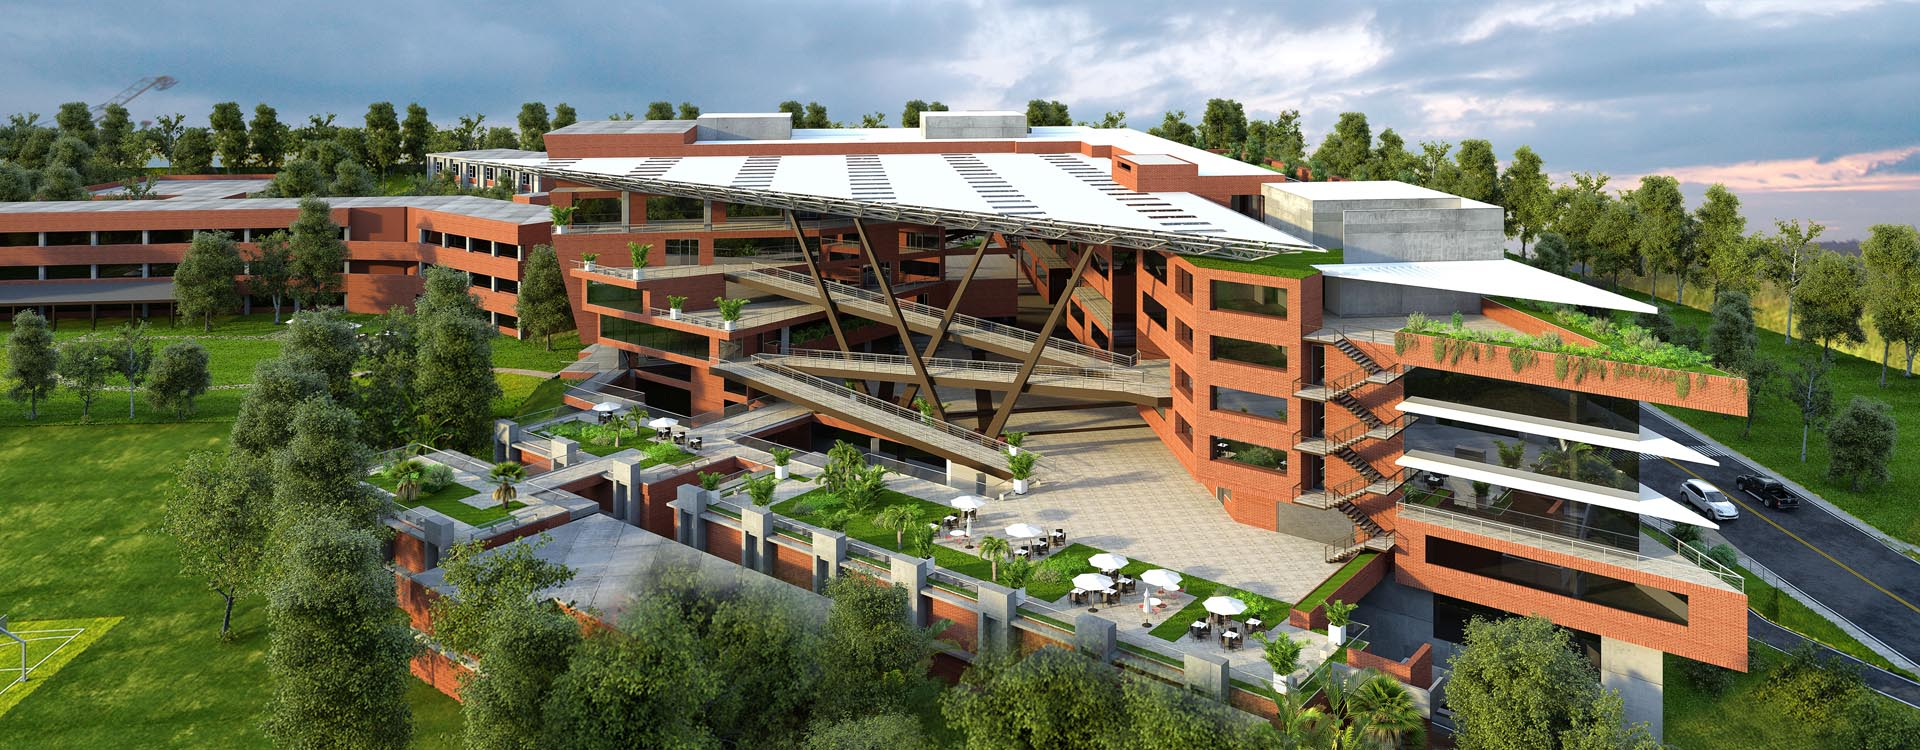
\includegraphics[height=13.25cm]{plantilla/portadacit.jpg}}
    	\makebox[\textwidth]{
    		\begin{overpic}[height=13.25cm]{\imagenportada}
     		\put(63,0){
\includegraphics[height=1.15in]{plantilla/fondologo_grande.png}}  
  			\put(64.5,2){
\includegraphics[height=0.55in]{plantilla/logoUVGblanco.eps}} 
        	\end{overpic}
    	}
    	%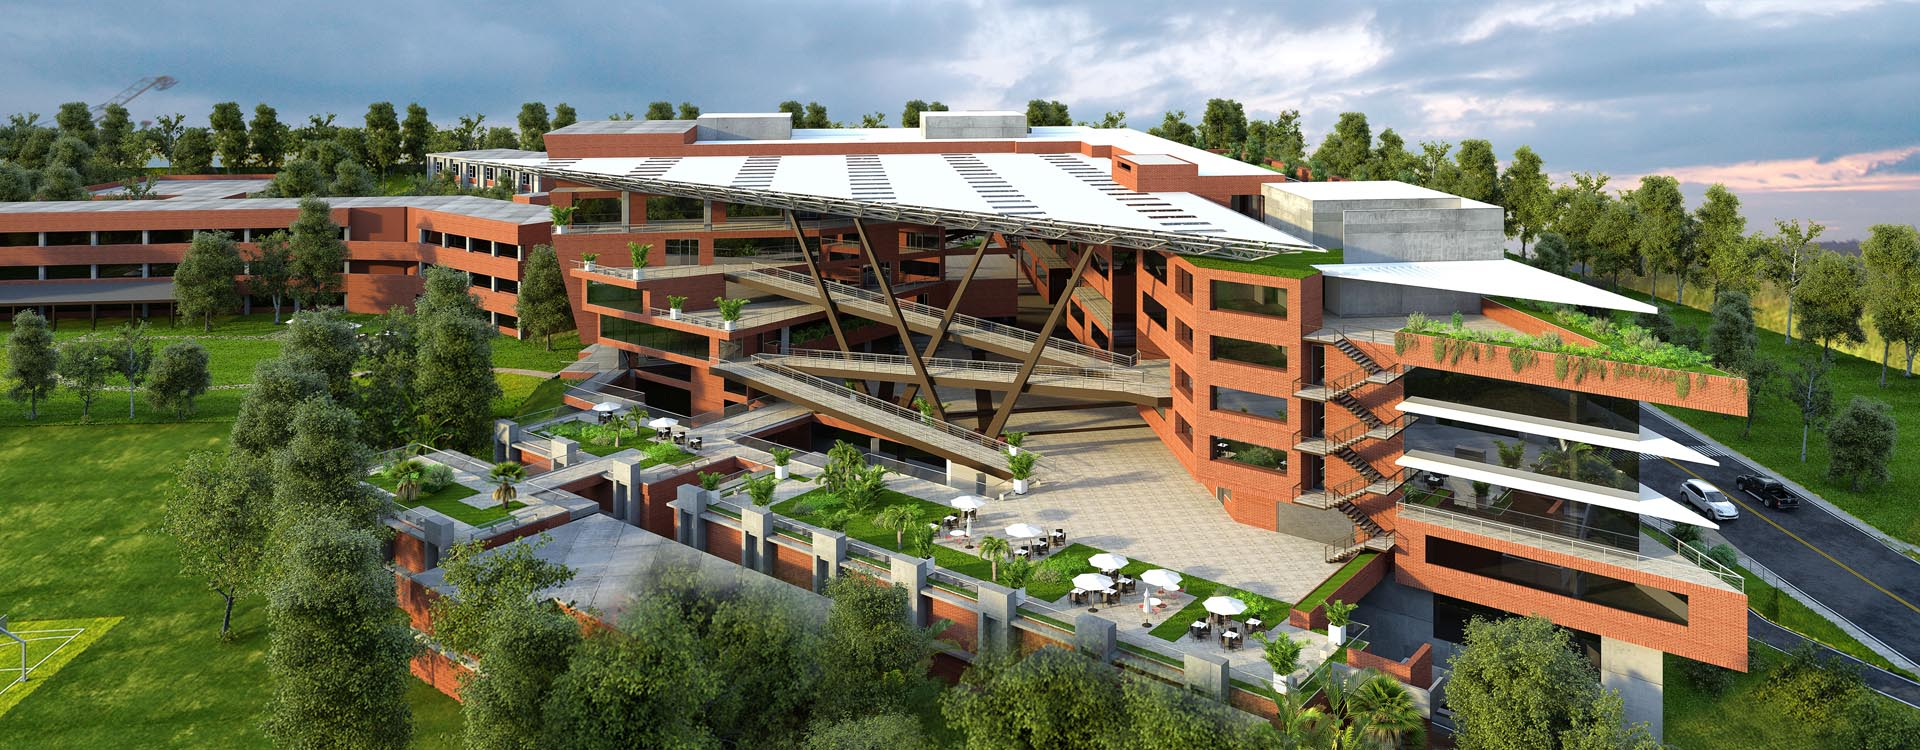
\includegraphics[height=13.25cm]{plantilla/portadacit.jpg}
	\end{figure}
	\restoregeometry
\fi

% ================================================================================
% PRIMERA PÁGINA
% ================================================================================
\ifdefined\CAPcaratula
	\newpage
%     \cleardoublepage\phantomsection
%     \pdfbookmark{Carátula}{toc}
	\pagecolor{white}
	\color{black}
	\setcounter{page}{1}
	\pagenumbering{roman}
	\thispagestyle{empty}
	\begin{center}
		\LARGE UNIVERSIDAD DEL VALLE DE GUATEMALA\\
		\LARGE Facultad de \uvgfacultad \\[0.75cm]
	\end{center}
	\begin{figure}[h]
		\begin{center}
		
\includegraphics[height=5.5 cm]{plantilla/escudoUVGnegro.eps}
		\vspace{0.5in}
		\end{center}
	\end{figure}
	\begin{center}
		\LARGE \textbf{\titulotesis} 
		\vfill
		\vfill
		\Large Trabajo de graduación en modalidad megaproyecto presentado por \\
		\Large \nombreestudiante \\
		\Large Para optar al grado académico de Licenciado en \uvgcarrera \\
		\vfill
		\large Guatemala, \mesentrega del \anoentrega
	\end{center}
\fi

% ================================================================================
% HOJA DE FIRMAS
% ================================================================================
\ifdefined\CAPfirmas
	\newpage
	\thispagestyle{empty}
	\vspace*{0.5in}
	\large Vo.Bo.:\\[1cm]
	\begin{center}
		(f) \rule[1pt]{4 in}{1pt}\\
		\nombreasesor
	\end{center}
	\vspace{1in}

	Tribunal Examinador:\\[1cm]
	\begin{center}
		(f) \rule[1pt]{4 in}{1pt}\\
		\nombreasesor \\[1in]
		(f) \rule[1pt]{4 in}{1pt}\\
		\nombreprimerex \\[1in]
		(f) \rule[1pt]{4 in}{1pt}\\
		\nombresegundoex
	\end{center}
	\vspace{1in}

	Fecha de aprobación: Guatemala, \fechaaprobacion.
	\normalsize
\fi

% ================================================================================
% CONTENIDO DEL TRABAJO
% ================================================================================
% PREFACIO
% --------------------------------------------------------------------------------
\ifdefined\CAPprefacio
	\newpage
	\cleardoublepage\phantomsection
    \chapter*{Prefacio}
    \ifdefined\parpordefecto
    	\defaultparformat{prefacio}
    \else
    	Desde una edad temprana, fui introducida al mundo de la lengua de señas por mi madre, quien me compartió no solo su experiencia aprendiendo esta lengua, sino también las dificultades y barreras que enfrentan las personas sordas. Recuerdo historias de cómo, en el pasado, a las personas sordas se les obligaba a articular palabras y leer labios, sin permitirles usar su propia forma de comunicación. Estas narrativas sembraron en mí una semilla de curiosidad y compasión que con el tiempo germinaría en un firme deseo de aportar algo significativo a la comunidad sorda.

Este compromiso se vio fortalecido por el invaluable apoyo y los recursos proporcionados por En-Señas Guatemala y ASEDES. A través de su colaboración, obtuve no solo material y datos fundamentales, sino también una profunda inspiración y apoyo constante, elementos esenciales para la realización de este proyecto. Estas instituciones y sus contribuciones han sido vitales para la realización de este proyecto.

Los principales desafíos que enfrenté incluyeron entender realmente las necesidades de las personas sordas. La falta de información disponible en internet me llevó a buscar conocimiento fuera de las fuentes tradicionales, involucrándome directamente con la comunidad sorda a través de clases y numerosas entrevistas. Este acercamiento personal fue crucial para conectar más profundamente con sus experiencias y entender cómo podría ayudar de manera efectiva.

Es mi esperanza que este trabajo ilumine no solo las dificultades diarias que enfrentan las personas sordas, sino también que iniciativas como ``Señas Chapinas'' contribuyan a superar barreras comunicativas. Aspiro a que los usuarios obtengan una visión genuina de la vida en la comunidad sorda y reconozcan la importancia de fomentar un entorno más inclusivo y accesible para todos.


    \fi
    \addcontentsline{toc}{chapter}{Prefacio}
\fi

% AGRADECIMIENTOS
% --------------------------------------------------------------------------------
\ifdefined\CAPagradecimientos
	\newpage
    \cleardoublepage\phantomsection
	\chapter*{Agradecimientos}
	\ifdefined\parpordefecto
    	\defaultparformat{agradecimientos}
    \else
    	Quiero expresar mi más sincero agradecimiento a todas las personas que han contribuido a la realización de este proyecto, cada una de las cuales ha sido fundamental en su desarrollo.

Primero, mi gratitud a mi asesor, el Ingeniero Dennis Aldana, por su invaluable guía y apoyo a lo largo de todo el proceso de investigación y redacción de este trabajo. Su dirección experta fue esencial para navegar los retos académicos y prácticos de este proyecto.

Un agradecimiento muy especial a mi madre, quien no solo me introdujo al mundo de la lengua de señas, sino que también me inspiró a embarcarme en este proyecto. Sus historias y experiencias han sido la chispa que encendió mi pasión por hacer una diferencia en la comunidad sorda.

Estoy profundamente agradecida con ASEDES, especialmente a Niurka Waleska Bendfeldt Rosada y Alain de León, por proporcionarme los materiales, las entrevistas y todos los recursos necesarios para llevar a cabo este trabajo. Su colaboración fue indispensable para entender mejor las necesidades y desafíos de la comunidad sorda.

Mi reconocimiento a las alumnas practicantes de ASEDES: Evelyn Cacao, Any Max y Ruth Amézquita, quienes generosamente permitieron que grabáramos sus señas, contribuyendo significativamente a la autenticidad y calidad del contenido de este proyecto.

Finalmente, un agradecimiento especial a Antonio Barrientos, Director General de En-Señas, y a Gabriela Velázquez, maestra de En-Señas. Ambos, además de introducirme prácticamente a la comunidad sorda, me recibieron en En-Señas para que aprendiera la lengua de señas, ayudándome a comprender profundamente sus necesidades y esperanzas. Su apertura y disposición para compartir su conocimiento y experiencia fueron cruciales para este proyecto.

A todos ustedes, mi más profundo respeto y gratitud por su apoyo y contribuciones.
    \fi 
	\addcontentsline{toc}{chapter}{Agradecimientos}
\fi

% ÍNDICE GENERAL
% --------------------------------------------------------------------------------
\ifdefined\CAPindice
	\newpage
    %\cleardoublepage\phantomsection
	\renewcommand{\contentsname}{Índice}
    \phantomsection
    \pdfbookmark{\contentsname}{toc}
	\tableofcontents
\fi

% LISTADO DE FIGURAS
% --------------------------------------------------------------------------------
\ifdefined\CAPfiguras
	\newpage
    \cleardoublepage\phantomsection
	\renewcommand{\listfigurename}{Lista de Figuras}
	\listoffigures
	\addcontentsline{toc}{chapter}{Lista de Figuras}
\fi

% LISTADO DE CUADROS
% --------------------------------------------------------------------------------
\ifdefined\CAPcuadros
	\newpage
    \cleardoublepage\phantomsection
	\renewcommand{\listtablename}{Lista de Cuadros}
	\listoftables
	\addcontentsline{toc}{chapter}{Lista de Cuadros}
\fi

% RESUMEN
% --------------------------------------------------------------------------------
\ifdefined\CAPresumen
	\newpage
    \cleardoublepage\phantomsection
	\chapter*{Resumen}
	\ifdefined\parpordefecto
		\defaultparformat{resumen}
	\else
		``Señas Chapinas'' es un proyecto innovador que responde a la necesidad crítica de mejorar la comunicación para los usuarios de LENSEGUA en Guatemala. Desarrollada como una aplicación móvil para Android, esta herramienta utiliza tecnologías de visión por computadora y aprendizaje profundo para traducir la lengua de señas guatemalteca a texto español. La aplicación está especialmente diseñada para cubrir vocabulario esencial, tanto para situaciones cotidianas como de emergencia, facilitando así las interacciones diarias y elevando la calidad de vida de la comunidad sorda.

A lo largo del desarrollo de ``Señas Chapinas'', se implementaron metodologías de diseño centradas en el usuario para crear una interfaz que no solo es funcional y accesible, sino también culturalmente relevante, reflejando la identidad guatemalteca para conectar profundamente con los usuarios. Este enfoque asegura que la aplicación no solo sea una herramienta de traducción, sino también un medio para fomentar la inclusión y el entendimiento cultural.

La colaboración activa con la comunidad sorda ha sido vital en todas las etapas del proyecto, desde la concepción hasta la implementación. Esta cooperación ha permitido que ``Señas Chapinas'' se desarrolle no solo como una solución tecnológica, sino como un recurso comunitario que promueve una mayor inclusión social y entendimiento.

Con ``Señas Chapinas'', se espera establecer un precedente para futuras innovaciones en tecnologías accesibles, demostrando cómo las herramientas adecuadamente diseñadas pueden superar barreras significativas y mejorar la interacción social dentro y fuera de la comunidad sorda.
	\fi
	\addcontentsline{toc}{chapter}{Resumen}
\fi

% INTRODUCCIÓN
% --------------------------------------------------------------------------------
\ifdefined\CAPintroduccion
	\newpage
	\pagenumbering{arabic}
	\setcounter{page}{1}
	\chapter{Introducción}
	\ifdefined\parpordefecto
		\defaultparformat{introduccion}
	\else
		Este proyecto surge de la necesidad de superar las barreras de comunicación para los usuarios de LENSEGUA. ``Señas Chapinas'' es una iniciativa que consiste en el desarrollo de una aplicación móvil para Android, diseñada para traducir lengua de señas a texto utilizando tecnologías avanzadas como visión por computadora y aprendizaje profundo. Con un enfoque en el vocabulario esencial para la vida cotidiana y situaciones de emergencia, la aplicación tiene como objetivo facilitar las interacciones diarias y mejorar la calidad de vida de la comunidad sorda. 

El módulo de diseño y desarrollo móvil se centra en crear una aplicación que ofrezca una experiencia de usuario agradable y una interfaz visualmente atractiva. Para esto, se implementó un plan de diseño que no solo asegura la funcionalidad y la accesibilidad, sino que también incorpora elementos visuales que reflejen la cultura guatemalteca, conectando así con los usuarios de una manera más profunda y significativa.

En colaboración con la comunidad sorda y con base en una retroalimentación constante, ``Señas Chapinas'' busca ser más que una aplicación; aspira a ser un recurso valioso que no solo mejore la comunicación, sino que también fomente una mayor inclusión y entendimiento dentro de la sociedad guatemalteca.

	\fi
\fi

% OBJETIVOS
% --------------------------------------------------------------------------------
\ifdefined\CAPobjetivos
	\newpage
	\chapter{Objetivos}
	\ifdefined\parpordefecto
		\defaultparformat{objetivos}
	\else
		\section{Objetivo General}
Diseñar y desarrollar "Señas Chapinas", una aplicación para dispositivos Android, que traduce la lengua de señas guatemalteca (LENSEGUA) a texto con gramática española. Esta herramienta busca eliminar las barreras comunicativas existentes en la actualidad, promoviendo la inclusión y mejorando significativamente las oportunidades de interacción social, educativa y laboral para personas sordas en Guatemala.

\section{Objetivos Específicos}
\begin{itemize}

\item Realizar una investigación de mercado y entrevistas con usuarios finales para comprender sus necesidades. Utilizar esta información para desarrollar perfiles de usuario detallados y diseñar flujos de usuario intuitivos y eficientes. 

\item Diseñar una interfaz enfocada en la retroalimentación constante de los usuarios, asegurando así una experiencia que responda a sus necesidades y expectativas. 

\item Desarrollar la aplicación ``Señas Chapinas'' en Android, implementando los prototipos e integrando los servicios externos para el procesamiento de videos y la traducción de lengua de señas.

\end{itemize}
	\fi
\fi

% JUSTIFICACIÓN
% --------------------------------------------------------------------------------
\ifdefined\CAPjustificacion
	\newpage
	\chapter{Justificación}
	\ifdefined\parpordefecto
		\defaultparformat{justificacion}
	\else
		La comunicación es un derecho fundamental y un pilar esencial para la interacción humana, indispensable en la educación, el trabajo y la participación activa en la sociedad \cite{NacionesUnidas2024}. Sin embargo, las barreras comunicativas aún limitan la interacción entre personas sordas y oyentes, restringiendo el acceso igualitario a oportunidades sociales y laborales. En respuesta a esta realidad, "Señas Chapinas" surge como una solución innovadora para superar estas barreras.

Aprovechando la amplia adopción de teléfonos inteligentes en Guatemala \cite{Xie2023}, donde la mayoría de estos dispositivos operan con el sistema Android \cite{Xie2023}, este proyecto busca desarrollar una aplicación móvil que actúe como un puente de comunicación eficiente y accesible. Esta aplicación pretende fortalecer la autonomía de las personas sordas y promover el uso de LENSEGUA.

El desarrollo de la aplicación involucra un análisis exhaustivo de las necesidades de los usuarios finales, recogiendo sus voces y experiencias mediante entrevistas y consultas. Este enfoque centrado en el usuario asegura que la aplicación responda adecuadamente a sus necesidades específicas. Además, se ha revisado cuidadosamente la legislación vigente, incluido el Decreto del Congreso de la República de Guatemala Número 3-2020, que reconoce la Lengua de Señas de Guatemala \cite{CongresoGuatemala2022}.

El propósito de ``Señas Chapinas'' es promover la inclusión laboral, facilitar el acceso a servicios esenciales y fomentar las interacciones sociales, contribuyendo así al enriquecimiento de la comunidad guatemalteca. Este proyecto es un avance significativo hacia la creación de una sociedad que valora la diversidad y proporciona igualdad de oportunidades para todos, utilizando tecnología móvil para superar las barreras de comunicación de manera eficiente y efectiva.

	\fi
\fi

% MARCO TEÓRICO
% --------------------------------------------------------------------------------
\ifdefined\CAPmarcoteorico
	\newpage
	\chapter{Marco Teórico}
	\ifdefined\parpordefecto
		\defaultparformat{marco_teorico}
	\else
		\section{Lengua de Señas}
Desde tiempos remotos, las personas con discapacidad auditiva han enfrentado significativos desafíos comunicativos, lo que les llevó a desarrollar su propio sistema de comunicación. Así surgió la lengua de señas, un conjunto estructurado de gestos visuales que permite a la comunidad sorda expresar ideas y emociones. Esta lengua, al igual que otras, está regida por normas lingüísticas establecidas por comunidades sordas \cite{MarzoPena2022}.

\subsection{Historia de la lengua de señas}
La lengua de señas se desarrolló de manera independiente por la comunidad sorda para satisfacer sus necesidades comunicativas. Históricamente estigmatizada y mal entendida, era considerada un lenguaje de gestos simple hasta que investigaciones realizadas en 1960 por William Stokoe revelaron su capacidad para expresar ideas complejas y estructuradas \cite{RodriguezVelasquezSF}.

En el siglo XVIII, el Abad Charles-Michel de L’Epée fundó la primera escuela pública para sordos, marcando un cambio trascendental en la educación de esta comunidad, utilizando la lengua de señas como principal medio de enseñanza. Este avance no solo facilitó la comunicación y el aprendizaje, sino que también permitió que los sordos desempeñaran roles activos como educadores. La metodología de L’Epée se expandió internacionalmente, influyendo en la creación de escuelas y en el desarrollo de nuevas lenguas de señas \cite{RodriguezVelasquezSF}.

Durante los siglos XIX y XX, las lenguas de señas ganaron reconocimiento como sistemas lingüísticos completos y estructurados, capaces de expresar una gama completa de ideas y emociones. En el siglo XX, el reconocimiento de los derechos lingüísticos de las comunidades sordas se amplió significativamente, afirmando la importancia de las lenguas de señas como herramientas educativas y culturales esenciales \cite{RodriguezVelasquezSF}.

A raíz de la necesidad de comunicación en las comunidades sordas, cada país ha desarrollado su propia lengua de señas, integrando a menudo estructuras de lenguas de señas extranjeras, como el \textit{American Sign Language (ASL)}, así como señas locales únicas. Esto ha dado lugar a que cada país, e incluso regiones dentro de los mismos, tengan su propia lengua de señas con estructuras gramaticales y léxicos distintos \cite{RuizVilla2022}.

\subsection{Lengua de Señas en la Actualidad}
En la actualidad, la lengua de señas se está adaptando a un entorno globalizado y tecnológicamente avanzado, donde las necesidades comunicativas evolucionan constantemente. Estos cambios han impulsado la creación de legislaciones, políticas, formación de asociaciones y el desarrollo de nuevas tecnologías destinadas a minimizar las barreras comunicativas. Un ejemplo significativo es la iniciativa de las Naciones Unidas al proclamar el 23 de septiembre como Día Internacional de las Lenguas de Señas, enfatizando la importancia de estas lenguas \cite{Parada2022}.

Sin embargo, a pesar de estos avances, persisten desafíos significativos. La falta de uniformidad de las lenguas de señas a nivel global requiere que las personas aprendan la lengua de señas específica de cada comunidad, lo cual impide la existencia de una forma de comunicación internacional uniforme \cite{RuizVilla2022}.

Además, la lengua de señas, a menudo catalogada como una lengua minoritaria, es aprendida solamente por una pequeña fracción de la población sin discapacidades auditivas. Esta limitada difusión crea una brecha de comunicación significativa, contribuyendo a la marginación de la comunidad sorda y limitando su participación plena en actividades sociales y económicas. Esto subraya la necesidad de una mayor educación y sensibilización sobre la lengua de señas para promover una verdadera inclusión \cite{MelendezLabrador2021}.

\section{Lengua de Señas de Guatemala (LENSEGUA)}
\subsection{Historia}
La Lengua de Señas de Guatemala (LENSEGUA) ha evolucionado como una herramienta vital de comunicación para la comunidad sorda guatemalteca. Aunque su desarrollo específico ha sido menos documentado en comparación con lenguas de señas de otros países, LENSEGUA ha sido influenciada tanto por “Señas Caseras ” de diferentes departamentos del país como por interacciones con lenguas de señas de otros países \cite{Aroche2022} \cite{EndangeredLanguages}.

Antes de la formalización del uso de LENSEGUA, no existía un manual estandarizado que facilitara el aprendizaje de la lengua de señas guatemalteca. Hoy en día de hecho todavía existen diferencias entre las señas utilizadas en los departamentos del país. Sin embargo, en julio de 2001, el Comité Pro Ciegos y Sordos de Guatemala, una institución pionera en la educación y rehabilitación de personas con discapacidad auditiva, publicó el primer manual oficial para el aprendizaje de LENSEGUA. Este manual representó un avance crucial en la estandarización y enseñanza de la lengua de señas, proporcionando un recurso esencial para los estudiantes, profesionales y la comunidad en general interesada en aprender este método de comunicación \cite{deLeon2021}.

\subsection{Legislación}
En términos legislativos, Guatemala ha hecho avances significativos en la última década. En 2020 el Congreso de la República de Guatemala mediante el Decreto 3-2020, reconoce oficialmente la Lengua de Señas de Guatemala como la lengua oficial para la comunicación en lengua de señas dentro del país. Este marco legal fue el resultado de los esfuerzos conjuntos de varias asociaciones que abogaron por su formalización, destacando la importancia de reconocer y apoyar la comunicación para las personas sordas en Guatemala \cite{CongresoGuatemala2020} .

El Decreto establece que todas las instituciones públicas y privadas deben garantizar la inclusión de la LENSEGUA como parte de su comunicación y servicios. Además, se promueve la educación bilingüe (español y LENSEGUA) en las escuelas que atienden a estudiantes sordos, asegurando así su derecho a una educación equitativa y accesible \cite{CongresoGuatemala2020}.

Este reconocimiento no solo valida a LENSEGUA como una lengua completa y estructurada, sino que también impulsa la creación de políticas y programas destinados a mejorar la accesibilidad en todos los aspectos de la vida pública para la comunidad sorda, desde la educación hasta el acceso a los servicios de salud y legales. El Decreto promueve la inclusión y asegura que las personas con discapacidad auditiva tengan acceso a la educación y la información en su lengua materna, libre de cualquier discriminación \cite{CongresoGuatemala2020}.

\subsection{Aprendizaje y Recursos}
LENSEGUA se puede aprender en varias instituciones y a través de recursos en línea que buscan facilitar el acceso y la difusión de esta lengua. Entre las principales entidades que ofrecen cursos y formación en LENSEGUA están \cite{LenseguaSF}:

\begin{itemize}
    \item ASEDES (Asociación Educativa para el Sordo)
    \item ASORGUA (Asociación de Sordos de Guatemala)
    \item Benemérito Comité Prociegos y Sordos de Guatemala
    \item En-Señas Guatemala
    \item CESGUA (Coordinación de Educación y Servicios en Guatemala)
    \item INTERGUA (Coordinación de intérpretes de lengua de señas de Guatemala)
    \item ANDYSISC (Servicios de interpretación profesional de Lengua de Señas)
    \item FUNDAL
    \item ONG Sordos Latinos Guatemala
\end{itemize}

Estas organizaciones no solo proporcionan educación en LENSEGUA, sino que facilitan una serie de conferencias y talleres impartidos por especialistas para personas con discapacidad auditiva \cite{LenseguaSF}.

\subsection{Gramática y Estructura}
La gramática y estructura de LENSEGUA reflejan una vasta complejidad lingüística que permite a los usuarios expresar una amplia gama de conceptos y emociones. Este sistema de comunicación es completo con su propia sintaxis, léxico y reglas gramaticales. Aquí se describen algunas de las características distintivas de LENSEGUA \cite{EnSenasCultura}  \cite{EnSenasGramatica} \cite{EnSenasTecnicas}  :

\begin{itemize}
    \item \textbf{Morfología}: La morfología en LENSEGUA utiliza modificadores manuales y no manuales para alterar el significado de los signos básicos, incluyendo modificaciones para indicar número, tiempo, aspecto, y otros atributos gramaticales.
    \begin{itemize}
        \item El signo para ``comer" podría modificarse para expresar ``comer mucho" mediante la repetición del signo o cambios en la expresión facial.
    \end{itemize}
    \item \textbf{Ausencia de género y artículos}: Como en muchas lenguas de señas, LENSEGUA no utiliza género gramatical ni artículos.
    \begin{itemize}
        \item Español: ``la casa", ``el perro".
        \item LENSEGUA signa ``casa" y ``perro" sin modificadores adicionales.
    \end{itemize}
    \item \textbf{No Uso de Preposiciones}: LENSEGUA omite preposiciones, que en español son cruciales para las relaciones espaciales o temporales. La relación se establece a través del contexto y la configuración de los signos.
    \begin{itemize}
        \item Español: ``en la casa".
        \item LENSEGUA: se usa gesto para indicar la ubicación relativa y el signo de casa.
    \end{itemize}
    \item \textbf{Omisión de Signos de Puntuación y Mayúsculas}: LENSEGUA no utiliza signos de puntuación ni mayúsculas. La escritura refleja una secuencia continua de signos, que se diferencia notablemente de la estructura del español.
    \begin{itemize}
        \item LENSEGUA: ``Disculpa mi hija no llega colegio porque muy enferma tiene tos gripe que en casa ya tomar medicinas”.
    \end{itemize}
    \item \textbf{Verbos No Conjugados}: En LENSEGUA, los verbos no se conjugan. El tiempo y el aspecto se indican con signos específicos al principio de la frase o a través de la expresión facial.
    \begin{itemize}
        \item Español: ``Yo estoy comiendo”.
        \item LENSEGUA: se signa ``yo comer”.
    \end{itemize}
    \item \textbf{Orden Gramatical}: El orden gramatical típico en LENSEGUA es Tiempo, Lugar, Sujeto, Objeto, Verbo (TLSOV), diferente al orden Sujeto, Verbo, Objeto (SVO) del español. Este orden facilita que el contexto temporal y espacial quede establecido claramente al inicio.
    \begin{itemize}
        \item Español: ``Yo ayer jugué futbol”.
        \item LENSEGUA: se signa ``pasado yo fútbol jugar”.
    \end{itemize}
\end{itemize}

\section{Diseño de Interfaz de Usuario (UI)}
\subsection{Definición de UI (Interfaz de Usuario)}
El diseño de la interfaz de usuario (UI) se dedica a la creación de los elementos visuales e interactivos de un producto digital. En esencia, se trata de diseñar lo que los usuarios ven en sus pantallas \cite{OrtegaSF}.

La interfaz de usuario determina en gran medida las primeras impresiones que tienen estos acerca de un negocio o producto. Cuando los usuarios pueden navegar fácilmente por una interfaz y completar las tareas deseadas, no solo mejora su experiencia, sino que también beneficia al negocio en general. Cuanto más visualmente atractiva y acogedora sea una interfaz, más probable es que atraiga a los usuarios y los motive a explorar más \cite{OrtegaSF}.

\subsection{Elementos de la Interfaz de Usuario}
Los elementos de la UI son los componentes básicos de las aplicaciones y sitios web con los que los usuarios interactúan. Estos elementos son esenciales para el desarrollo de funcionalidades óptimas y una experiencia de navegación agradable. Los elementos UI se agrupan en tres categorías principales \cite{OrtegaSF}:

\begin{itemize}
    \item \textbf{Elementos de entrada}: Permiten a los usuarios ingresar información en el sistema y, en ocasiones, son parte del proceso de validación de entrada. Los elementos de entrada más comunes incluyen \cite{OrtegaSF}:
    \begin{itemize}
        \item Listas desplegables
        \item Campos de texto o contraseña
        \item Selectores de fecha
        \item Casillas de verificación
        \item Diálogos de confirmación
    \end{itemize}
    \item \textbf{Elementos de salida}: Muestran los resultados basados en las entradas del usuario y las operaciones previas. Ejemplos de elementos de salida son \cite{OrtegaSF}:
    \begin{itemize}
        \item Alertas
        \item Mensajes de éxito
        \item Mensajes de error
    \end{itemize}
    \item \textbf{Elementos auxiliares}: Proporcionan información adicional al usuario y mejoran la navegación. Estos elementos se dividen en tres subcategorías \cite{OrtegaSF}:
    \begin{itemize}
        \item \textbf{Elementos de navegación}: Facilitan el desplazamiento a través del producto digital \cite{OrtegaSF}. Algunos ejemplos son:
        \begin{itemize}
            \item Menús de navegación
            \item Listas de enlaces
        \end{itemize}
        \item \textbf{Elementos informativos}: Incluyen referencias que ayudan a utilizar o comprender el producto digital \cite{OrtegaSF}. Ejemplos son:
        \begin{itemize}
            \item Iconos
            \item Notificaciones
        \end{itemize}
        \item \textbf{Elementos de grupos o contenedores}: Ayudan a organizar y mantener los componentes del producto juntos \cite{OrtegaSF}. Ejemplos incluyen:
        \begin{itemize}
            \item Barras laterales
            \item Contenedores de contenido
        \end{itemize}
    \end{itemize}
\end{itemize}

\subsection{Estándares de Diseño}
\subsubsection{Tamaño y Posición de Botones}
El tamaño de los objetos táctiles en una aplicación móvil es crucial, ya que afecta directamente la facilidad con la que los usuarios pueden interactuar con la interfaz. Si los botones no tienen un tamaño y espacio óptimos, los usuarios podrían no alcanzar su objetivo o presionar el botón equivocado \cite{Bustos2022}.

Investigaciones sobre el tamaño y el espaciado de los botones han establecido estándares que funcionan para la mayoría de los usuarios. Los estudios encontraron que los usuarios tienen la menor precisión táctil en botones de menos de 42 píxeles, los cuales se usan generalmente para funciones de baja prioridad. La mayor precisión se encontró en botones de entre 42 y 72 píxeles. Por ello, se utilizan botones de aproximadamente 60 píxeles para funciones de prioridad media, mientras que los de más de 72 píxeles se reservan para funciones de alta prioridad, asegurando así la accesibilidad para todos los usuarios \cite{Anthony2019}.

Además del tamaño, existen ciertos márgenes y áreas táctiles recomendadas alrededor de los botones para garantizar que sean fácilmente accesibles y utilizables. Estos márgenes aseguran que haya suficiente espacio alrededor de los botones para evitar errores de pulsación. Dependiendo del tamaño del botón, se recomienda un margen de 12 a 24 píxeles para botones grandes, de 24 a 36 píxeles para botones medianos y de 36 a 48 píxeles para botones pequeños \cite{Anthony2019}. 

\begin{figure}[!h]
    \centering
    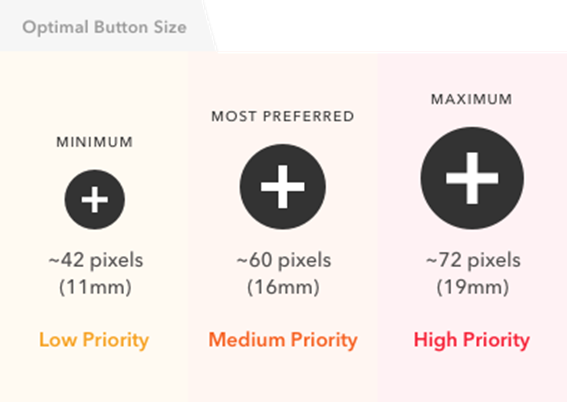
\includegraphics[width=0.5\linewidth]{figuras/optimal_button_size.png}
    \caption{Tamaño óptimo de botones según su prioridad}
    \label{fig:botones_optimos}
\end{figure}


Asimismo, la ubicación de los botones es fundamental para la usabilidad. Los usuarios están acostumbrados a interactuar con dispositivos digitales a lo largo del día y tienden a buscar ciertos elementos en ubicaciones predecibles. Por esta razón, es importante posicionar los botones en lugares donde los usuarios esperan encontrarlos, como en la parte inferior de la pantalla para acciones frecuentes o en la esquina superior derecha para opciones adicionales. Esta previsibilidad mejora la eficiencia y reduce la frustración del usuario \cite{Pickaso2022}.

\begin{figure} [h]
    \centering
    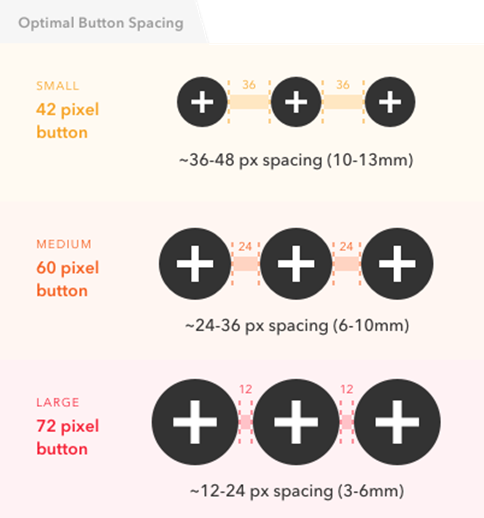
\includegraphics[width=0.5\linewidth]{figuras/optimal_space_buttons.png}
    \caption{Espaciado óptimo de botones según su tamaño}
    \label{fig:esapcio_optimo}
\end{figure}


\subsubsection{Diseño Responsivo}
El diseño responsivo es crucial para aplicaciones móviles, ya que asegura que la interfaz se adapte a diferentes tamaños de pantalla y resoluciones \cite{Becos2024}.

Dado que las pantallas de los dispositivos móviles varían en densidad, con más píxeles por pulgada en pantallas de mayor resolución, es importante utilizar píxeles independientes de la densidad (dp) para definir las dimensiones de los elementos de la interfaz. Esto asegura que los elementos mantengan su tamaño y proporción adecuados en diferentes dispositivos, proporcionando uniformidad y coherencia visual \cite{Pickaso2022}.

\subsubsection{Principios de Diseño}
Hay una serie de principios de diseño de interfaces para lograr que el producto digital satisfaga al cliente final \cite{AnonimoUX}.

\begin{itemize}
    \item \textbf{Simplicidad}: Es crucial evitar elementos innecesarios que puedan causar confusión \cite{AnonimoUX}.
    \item \textbf{Consistencia}: Al emplear elementos comunes en la interfaz de usuario, los usuarios se sienten más cómodos y familiarizados con el diseño, lo que facilita el uso del producto digital \cite{AnonimoUX}.
    \item \textbf{Jerarquía y manejo de espacios}: La disposición y estructuración de los elementos según su importancia ayuda a dirigir la atención del usuario a la información más relevante. Agrupar elementos relacionados crea una relación visual y mejora la comprensión del contenido \cite{AnonimoUX}.
    \item \textbf{Color y tipografía}: El color es esencial en el diseño de interfaces. Ajustar la saturación, luz y contraste del color en el diseño destaca elementos importantes y facilita la navegación. Asimismo, se utilizan diferentes tamaños, fuentes y disposiciones del texto para mejorar la legibilidad y jerarquía visual \cite{AnonimoUX}.
\end{itemize}

\subsubsection{Paleta de Colores}
Los colores desempeñan un papel fundamental en el diseño de interfaces de usuario, ya que no solo aportan personalidad y estilo al producto digital, sino que también influyen en la percepción y emociones del usuario \cite{EspacioUXSF}.

Una paleta de colores bien diseñada ayuda a los usuarios a comprender rápidamente la importancia y la relación entre diferentes elementos en la interfaz, como las llamadas a la acción o la información crítica. Al asignar colores específicos a distintas categorías o secciones, los usuarios pueden identificar fácilmente su ubicación en la interfaz y cómo navegar dentro de ella \cite{EspacioUXSF}.

La paleta de colores se elige para evocar emociones específicas que se alineen con los objetivos del diseño. Por ejemplo, los colores cálidos como el rojo y el naranja pueden provocar sensaciones de urgencia o excitación, lo que los hace ideales para botones de compra o alertas. En contraste, los colores fríos como el azul y el verde pueden inducir sensaciones de tranquilidad y confianza, siendo perfectos para páginas de inicio o secciones de información \cite{EspacioUXSF}.

Es esencial que la paleta de colores tenga en cuenta la legibilidad y la visibilidad, cumpliendo con los estándares de contraste y asegurando que la información sea clara para todos los usuarios \cite{EspacioUXSF}.

\subsubsection{Selección de Tipografía}
Al igual que la paleta de colores, la elección de una tipografía tiene un impacto significativo en el diseño de un producto digital. La tipografía moldea la manera en que se percibe y comprende la información visual. Elementos tipográficos como el tipo de letra, su tamaño y color tienen la capacidad de transmitir diversos significados y causar distintas respuestas emocionales \cite{CamaraSevilla2023}.

Una tipografía bien elegida mejora y facilita la comprensión y asimilación de la información por parte de los usuarios. Por ejemplo, una fuente en negrita y con letras mayúsculas puede transmitir fuerza y determinación, mientras que una tipografía delicada y manuscrita puede evocar elegancia y sofisticación. En contraste, una tipografía inadecuada puede dificultar la lectura, causar fatiga visual e incluso generar confusión o frustración en el usuario \cite{CamaraSevilla2023}.

Las tipografías se pueden clasificar según sus características:

\begin{itemize}
    \item \textbf{Fuentes Serif}: Estas fuentes se caracterizan por tener pequeños remates en los extremos de las letras, transmitiendo una sensación de formalidad. Ejemplos populares incluyen Times New Roman y Georgia \cite{CamaraSevilla2023}.
    \item \textbf{Fuentes Sans Serif}: Carecen de remates, lo que les confiere una apariencia más moderna y limpia. Se utilizan comúnmente en proyectos digitales. Ejemplos comunes son Arial, Helvetica y Calibri \cite{CamaraSevilla2023}.
    \item \textbf{Fuentes Script o Manuscritas}: Estas fuentes imitan la escritura a mano y suelen transmitir una sensación de personalización y creatividad. Ejemplos incluyen Brush Script y Pacifico \cite{CamaraSevilla2023}.
    \item \textbf{Fuentes Decorativas}: Son variadas y altamente estilizadas, utilizadas con fines ornamentales y para llamar la atención. Pueden ser temáticas o artísticas, como las fuentes de Navidad o títulos de películas \cite{CamaraSevilla2023}.
    \item \textbf{Fuentes Monoespaciadas}: Cada carácter ocupa el mismo espacio horizontal, lo que es útil en programación y diseño de tablas. Ejemplos son Courier New y Consolas \cite{CamaraSevilla2023}.
    \item \textbf{Fuentes Display}: Estas fuentes son diseñadas para títulos y encabezados, siendo llamativas y de alto impacto visual. Ejemplos incluyen Impact y Lobster \cite{CamaraSevilla2023}.
    \item \textbf{Fuentes Dingbats}: Contienen símbolos y caracteres especiales en lugar de letras y números, útiles para la creación de iconos y elementos gráficos. Wingdings y Webdings son ejemplos conocidos \cite{CamaraSevilla2023}.
\end{itemize}

Seleccionar la tipografía correcta es esencial para asegurar que el mensaje se transmita de manera eficaz y atractiva para los productos digitales. Hay varios factores clave que se deben considerar para conseguirlo \cite{CamaraSevilla2023}:

\begin{itemize}
    \item \textbf{Legibilidad}: La tipografía debe ser fácil de leer para el público objetivo. Esto incluye considerar el tamaño de la fuente, el espaciado entre letras y palabras, y la claridad de las formas de las letras \cite{CamaraSevilla2023}.
    \item \textbf{Personalidad}: La tipografía debe reflejar la identidad y los valores del producto digital \cite{CamaraSevilla2023}.
    \item \textbf{Consistencia}: Mantener una apariencia uniforme a lo largo del diseño refuerza la identidad visual y facilita la navegación del usuario \cite{CamaraSevilla2023}.
    \item \textbf{Jerarquía}: Utilizar variaciones en la tipografía, como tamaños y estilos (negritas, cursivas), para establecer una jerarquía de información ayuda a los usuarios a identificar elementos clave como títulos, subtítulos y texto principal \cite{CamaraSevilla2023}.
    \item \textbf{Combinación de Fuentes}: Seleccionar dos o más fuentes que se complementen puede enriquecer el diseño \cite{CamaraSevilla2023}.
    \item \textbf{Tamaño y Espaciado}: El tamaño de la fuente y el espaciado entre líneas afectan la legibilidad y la estética \cite{CamaraSevilla2023}.
\end{itemize}

\section{Experiencia de Usuario (UX)}
\subsection{Definición de UX (Experiencia de Usuario)}
La experiencia de usuario (UX) se refiere a las percepciones, sentimientos y respuestas que los usuarios tienen al interactuar con un producto digital \cite{Chacon2024}.

\subsection{Diferencias entre UX y UI}
El diseño de interfaz de usuario (UI) y la experiencia de usuario (UX) son conceptos estrechamente relacionados, pero tienen enfoques distintos y desempeñan roles específicos en el desarrollo de productos digitales. Mientras que UX se enfoca en el recorrido y en las interacciones de un usuario en todo el producto digital, UI se centra en cómo se ve y funciona el producto \cite{Chacon2024}.

\subsection{Tipos de experiencia de usuario}
Existen diferentes tipos de experiencia que pueden influir en cómo un usuario percibe un producto digital:

\begin{itemize}
    \item \textbf{Experiencia de navegación}: Se refiere a la forma en que un usuario se desplaza por un producto digital. Incluye la estructura de la navegación y la lógica que conecta las diferentes secciones o páginas. Una navegación intuitiva permite a los usuarios encontrar rápidamente la información que buscan. Por ejemplo, un menú de navegación claro y bien organizado facilita el movimiento entre las distintas secciones de una aplicación \cite{Chacon2024}.
    \item \textbf{Experiencia de usabilidad}: Se enfoca en cómo los usuarios interactúan con los elementos del producto digital. La usabilidad asegura que todos los componentes, como botones, barras de desplazamiento y formularios, funcionen correctamente y de manera consistente. Por ejemplo, un botón que responde rápidamente al ser presionado y realiza la acción esperada contribuye a una experiencia de usuario positiva \cite{Chacon2024}.
    \item \textbf{Experiencia Sensorial}: Involucra los elementos que impactan sensorialmente al usuario, como colores, disposición de elementos, sonidos y animaciones. Estos factores pueden influir significativamente en la percepción emocional del usuario respecto al producto. Por ejemplo, colores suaves y animaciones fluidas pueden crear una sensación de tranquilidad y profesionalismo, mientras que colores vibrantes y sonidos dinámicos pueden generar una sensación de energía y entusiasmo \cite{Chacon2024}.
\end{itemize}

\subsection{Proceso de experiencia de usuario}
La construcción de la experiencia de usuario para un producto se divide en varias etapas, cada una con su propio conjunto de actividades y herramientas \cite{Leon2013}:

\begin{itemize}
    \item \textbf{Investigación}: En esta etapa, se evalúan las necesidades de los clientes y se recopilan datos cruciales para entender mejor el contexto y las expectativas del usuario. Las técnicas más comunes incluyen \cite{Leon2013}:
    \begin{itemize}
        \item \textbf{Entrevistas:} Proveen información detallada directamente de los usuarios, ayudando a entender sus necesidades, deseos y problemas específicos \cite{Semi2022}.
        \item \textbf{Encuestas y Cuestionarios:} Recogen datos cuantitativos de una muestra más grande de usuarios, permitiendo identificar tendencias y patrones  \cite{Semi2022}.
        \item \textbf{Personas:} Creación de arquetipos basados en datos reales para representar diferentes tipos de usuarios  \cite{Semi2022}.
        \item \textbf{Mapas de Empatía:} Herramientas visuales que ayudan a comprender mejor a los usuarios, enfocándose en lo que piensan, sienten, dicen y hacen  \cite{Semi2022}.
        \item \textbf{Mapa de Experiencia del cliente:} Ilustra la experiencia completa de un usuario con un producto  \cite{Semi2022}.
        \item \textbf{Planteamiento del problema:} Define claramente los desafíos que el producto debe abordar  \cite{Semi2022}.
        \item \textbf{Diagramas de afinidad:} Organizan y agrupan información en categorías significativas  \cite{Semi2022}.
        \item \textbf{Análisis de la competencia:} Recopila información sobre tecnologías similares y reseñas de productos existentes  \cite{Semi2022}.
    \end{itemize}

\begin{figure}[h]
    \centering
    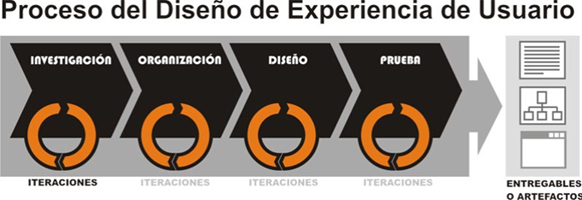
\includegraphics[width=0.5\linewidth]{figuras/proceso_diseno.png}
    \caption{Proceso de Diseño de Experencia de Usuario}
    \label{fig:enter-label}
\end{figure}

    
    \item \textbf{Organización}: Organiza toda la información obtenida durante la etapa de investigación utilizando herramientas como \cite{Leon2013}:
    \begin{itemize}
        \item \textbf{Mapa de Sitio:} Describe las páginas principales de un sitio y su relación, mostrando cómo se conectan  \cite{Semi2022}.
        \item \textbf{Flujo de Usuarios:} Diagrama que muestra la ruta que tomará un usuario en una aplicación para completar una tarea  \cite{Semi2022}.
        \item \textbf{Estructura Alámbrica/ Wireframes:} Visualización 2D de un producto digital, que va desde bocetos básicos a lápiz hasta diseños digitales interactivos (de baja, media y alta fidelidad)  \cite{Semi2022}.
    \end{itemize}
    \item \textbf{Diseño}: En la etapa de creación de prototipos, los wireframes de alta fidelidad se transforman en demostraciones interactivas que simulan fielmente la apariencia y el comportamiento del producto. Aquí se integra la investigación realizada en UI, considerando colores, tipografía, tamaños y espaciado de elementos, iconografía, entre otros. Las herramientas utilizadas incluyen Figma, Sketch y Adobe XD  \cite{Semi2022}.
    \item \textbf{Prueba}: Al finalizar la implementación, se realizan pruebas para asegurar que el producto cumple con las necesidades y expectativas de los usuarios  \cite{Semi2022}.
\end{itemize}

\section{Desarrollo Móvil en Android}
\subsection{Razones para elegir Android como plataforma de desarrollo}
Una de las razones principales para elegir Android como plataforma de desarrollo es su alta popularidad Guatemala. Según estudio la mayoría de celulares usados en el país son Samsung y Huawei, los cuales tienen sistema operativo Android \cite{Anonimo2019}.

Según datos recientes, Android domina el tráfico web móvil en el país, con un 82.50\% de participación. Esto significa que la mayoría de los usuarios de dispositivos móviles en Guatemala utilizan este sistema operativo, lo que amplía significativamente el alcance y la accesibilidad del producto desarrollado en esta plataforma \cite{Shum2023}.

\begin{figure} [h]
    \centering
    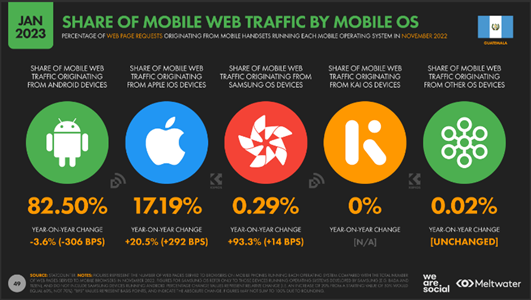
\includegraphics[width=0.5\linewidth]{figuras/mobile_web_traffic.png}
    \caption{Cuota de tráfico web móvil por sistema operativo}
    \label{fig:enter-label}
\end{figure}

Asimismo, Android es conocido por su diversidad en términos de dispositivos, desde teléfonos de alta gama hasta opciones más accesibles. También ofrece un alto nivel de flexibilidad y opciones de personalización, lo que facilita el desarrollo de aplicaciones. Finalmente, el ecosistema de desarrollo de Android está soportado con una vasta cantidad de recursos, herramientas y una comunidad activa de desarrolladores \cite{AnonimoAndroid}.

\subsection{Arquitectura de aplicaciones Android}
La arquitectura de una aplicación Android se basa en el patrón Modelo - Vista - Controlador (MVC). Aunque es muy común utilizar MVVM (Modelo - Vista - ViewModel), pues ofrece una separación más clara de la lógica de presentación y facilita el mantenimiento en comparación con MVC \cite{RamosSF}.

\subsubsection{Componentes}
\begin{itemize}
    \item \textbf{Modelo}: Contiene los datos, el estado y la lógica del negocio \cite{Bhadoria2013}.
    \item \textbf{Vista}: Representa la interfaz de usuario. Se comunica con el ViewModel a través de mecanismos de enlace de datos (data binding), permitiendo una actualización automática de la UI cuando cambian los datos \cite{Bhadoria2013}.
    \item \textbf{ViewModel}: Actúa como un intermediario entre el Modelo y la Vista. Expone datos y comandos que la Vista puede consumir y ejecutar, y notifica a la Vista sobre cambios en los datos utilizando observables (como LiveData) \cite{Bhadoria2013}.
\end{itemize}

\subsubsection{Flujo de Trabajo}
\begin{itemize}
    \item La Vista se enlaza automáticamente al ViewModel para observar los datos \cite{Bhadoria2013}.
    \item El ViewModel obtiene los datos del Modelo y prepara la lógica de presentación \cite{Bhadoria2013}.
    \item Cualquier cambio en el Modelo se refleja automáticamente en la Vista a través del ViewModel \cite{Bhadoria2013}.
    \item La interacción del usuario en la Vista invoca métodos en el ViewModel, que a su vez pueden actualizar el Modelo \cite{Bhadoria2013}.
\end{itemize}

\begin{figure}
    \centering
    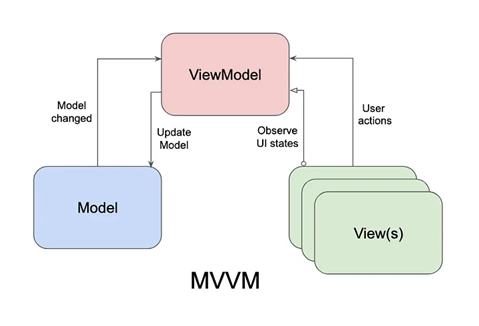
\includegraphics[width=0.5\linewidth]{figuras/mvvm.png}
    \caption{Diagrama de funcionamiento MVVM}
    \label{fig:enter-label}
\end{figure}

\subsection{Buenas prácticas de desarrollo Android}
Al desarrollar aplicaciones para Android, es esencial seguir ciertas buenas prácticas para asegurar la calidad y la eficiencia del producto final \cite{PhillipsStewart2022}:

\subsubsection{Uso de Layouts Adecuados}
\begin{itemize}
    \item \textbf{ConstraintLayout}: Es eficiente y flexible, permitiendo posicionar elementos de manera relativa a otros elementos \cite{PhillipsStewart2022}.
    \item \textbf{LinearLayout}: Organiza los elementos en una sola fila o columna, siendo útil para diseños sencillos y alineaciones básicas \cite{PhillipsStewart2022}.
    \item \textbf{RelativeLayout}: Permite posicionar los elementos en relación a otros elementos o a sus propios padres, ofreciendo más flexibilidad pero con un mayor costo de rendimiento comparado con ConstraintLayout \cite{PhillipsStewart2022}.
\end{itemize}

\subsubsection{Gestión de Recursos}
\begin{itemize}
    \item Utilizar unidades independientes de densidad (dp) para asegurar que los elementos de la interfaz mantengan su tamaño y proporciones adecuadas en dispositivos con diferentes tamaños de pantalla \cite{PhillipsStewart2022}.
    \item Definir colores, estilos y dimensiones en archivos de recursos para promover la reutilización y mantener la consistencia del diseño \cite{PhillipsStewart2022}.
    \item Utilizar Gradle para gestionar dependencias, lo que te permitirá mantener el código actualizado y seguro \cite{PhillipsStewart2022}.
\end{itemize}

\subsubsection{Optimización del Rendimiento}
\begin{itemize}
    \item Minimizar el uso de vistas anidadas para mejorar el rendimiento de la interfaz de usuario \cite{PhillipsStewart2022}.
    \item Evitar operaciones pesadas en el hilo principal \cite{PhillipsStewart2022}.
\end{itemize}

\subsubsection{Seguridad}
\begin{itemize}
    \item Proteger los datos del usuario mediante el uso de almacenamiento cifrado y permisos adecuados \cite{PhillipsStewart2022}.
    \item Validar las entradas del usuario para prevenir ataques de inyección y otras vulnerabilidades de seguridad \cite{PhillipsStewart2022}.
    \item Validar permisos de uso de almacenamiento, cámara, micrófono, etc para respetar las políticas de privacidad de Android \cite{PhillipsStewart2022}.
\end{itemize}


	\fi
\fi


% METOLOGIA
% --------------------------------------------------------------------------------
\ifdefined\CAPmetodologia
	\newpage
	\chapter{Metodología}
	\ifdefined\parpordefecto
		\defaultparformat{metodologia}
	\else
		\section{INVESTIGACIÓN DE MERCADO}

\subsection{Investigación y revisión sobre aplicaciones y tecnologías similares}

Se investigan aplicaciones con funcionalidades parecidas a la solución propuesta por Señas Chapinas. 

\subsubsection{Hand Talk Translator}

Es una aplicación gratuita para dispositivos Android e iOS diseñada para mejorar la comunicación entre la comunidad sorda y las personas que pueden oír. Esta traduce texto, ya sea en texto o en audio, al lenguaje de señas americanas. Esto se realiza por medio de Hugo, un avatar tridimensional animado por IA, que facilita la traducción y el aprendizaje. Los usuarios tienen la opción de repetir las traducciones, modificar la velocidad de Hugo, guardar y calificar sus traducciones preferidas. También pueden crear mensajes en GIF para compartir y personalizar la apariencia de Hugo en su tienda \cite{Foggetti2023}.

    
\begin{itemize}
    \item \textbf{Funcionalidades destacadas}
    \begin{itemize}
        \item Traducción de frases a lengua de señas ASL mostrado a través de animación 3D.
        \item Opción de compartir por GIF en redes sociales.
        \item Opción de guardar traducción en favoritos.
        \item Opción de repetir la traducción y cambiar la velocidad de reproducción.
    \end{itemize}
    
    \item \textbf{Características de Diseño}
    \begin{itemize}
        \item Incorpora elementos interactivos y de personalización para mejorar la experiencia del usuario. Esto vuelve la aplicación más atractiva y personal.
        \item Animación fluida de Hugo, que facilita el seguimiento visual de las señas.
        \item Interfaz intuitiva y simple que permite una navegación sencilla por las distintas funciones de la aplicación.
        \item Uso de color naranja que induce calidez, alegría, optimismo y confianza.
        \item Los íconos y botones son grandes y están claramente etiquetados, lo cual es útil para una rápida identificación de la funcionalidad.
        \item La interfaz es responsiva.
    \end{itemize}

    \item \textbf{Comentarios de usuarios}
    \begin{itemize}
        \item Los usuarios solicitan que la aplicación traduzca palabras y no letra por letra.
        \item Los usuarios solicitan mayor cantidad de palabras disponibles para traducción a señas.
    \end{itemize}
\end{itemize}

\begin{figure} [h]
    \centering
    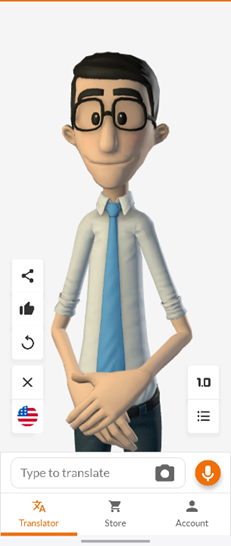
\includegraphics[width=0.25\linewidth]{figuras/handTalk.png}
    \caption{Muestra de aplicación “Hand Talk Translator”}
    \label{fig:enter-label}
\end{figure}


\subsubsection{SLAIT – Real-time Sign Language Translator with AI}

Es una aplicación en fase beta que ofrece servicios de traducción de lengua de señas americanas en tiempo real para dispositivos móviles, web, entre otros. Utiliza inteligencia artificial para realizar traducciones en tiempo real, otorgando facilidad de comunicación para comunicación diaria, salud, educación y oficina. Esta aplicación tendrá modalidad de pago, aunque permite ser parte de la aplicación beta sin costo pero con previo análisis del caso por la empresa \cite{SLAIT}.

\begin{itemize}
    \item \textbf{Funcionalidades destacadas}
    \begin{itemize}
        \item Traducción instantánea de voz a texto.
        \item Traducción instantánea de señas a texto.
    \end{itemize}

    \item \textbf{Características de Diseño}
    \begin{itemize}
        \item Diseño simple y amigable con el usuario.
    \end{itemize}
\end{itemize}

\begin{figure} [H]
    \centering
    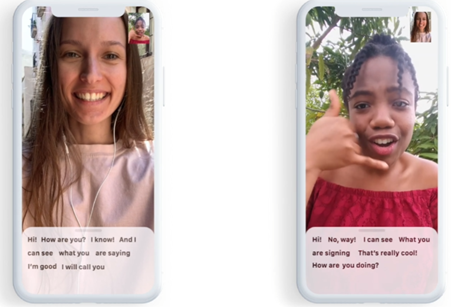
\includegraphics[width=0.5\linewidth]{figuras/slait.png}
    \caption{Muestra de aplicación “SLAIT”}
    \label{fig:enter-label}
\end{figure}

\subsubsection{Lenguaje de Señas IA}

La aplicación ofrece una plataforma de traducción de señas ASL a texto y viceversa, con múltiples funciones como búsqueda por categoría, emoji y alfabeto, y soporte para diez idiomas. Con más de 2,600 señas reconocidas, busca facilitar la comunicación y el aprendizaje del lenguaje de señas \cite{LenguajeDeSeñasIA}.

\begin{itemize}
    \item \textbf{Funcionalidades destacadas}
    \begin{itemize}
        \item Grabación de señas ASL para su reconocimiento y traducción a 10 diferentes idiomas.
        \item Traducción de frases en inglés a señas ASL, seña por seña.
        \item Búsqueda de señas por emoji, categoría, palabra y alfabéticamente.
    \end{itemize}

    \item \textbf{Características de Diseño}
    \begin{itemize}
        \item Paleta de colores e iconografía básica.
        \item Diseño confuso y apretado.
    \end{itemize}
\end{itemize}

\begin{figure}[H]
    \centering
    
\includegraphics[width=0.2\linewidth]{figuras/applenguasenasia.png}
    \caption{Muestra de aplicación “Lenguaje de señas IA”}
    \label{fig:enter-label}
\end{figure}

\subsubsection{AI Sign: Sign Language}

Es una aplicación para IOS que utiliza inteligencia artificial para reconocer más de 100 señas americanas. Tiene dos modos: reconocimiento de acciones en tiempo real y captura de datos para mejorar la precisión del modelo de aprendizaje automático \cite{AISign2023}.

\begin{itemize}
    \item \textbf{Funcionalidades destacadas}
    \begin{itemize}
        \item Capacidad de reconocimiento en tiempo real.
        \item Contiene un modo de ayuda y ajustes de configuración para personalizar la experiencia.
    \end{itemize}

    \item \textbf{Características de diseño}
    \begin{itemize}
        \item Muestra de toma de datos de las señas, señalando puntos clave de la mano.
        \item No hay paleta de colores, se usan elementos gráficos básicos.
        \item Botones poco amigables y descriptivos.
    \end{itemize}
\end{itemize}


\begin{figure} [H]
    \centering
    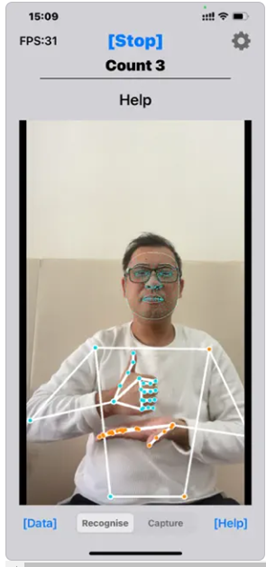
\includegraphics[width=0.25\linewidth]{figuras/ai_sign.png}
    \caption{Muestra de aplicación “AI Sign: Sign Language”}
    \label{fig:enter-label}
\end{figure}

\subsubsection{Sign Language Translator AI}

Es una aplicación móvil diseñada para reconocer y traducir el lenguaje de señas coreano. Utiliza inteligencia artificial para interpretar señas en tiempo real, buscando facilitar la comunicación para las personas sordomudas. La aplicación también fomenta la participación de los usuarios para mejorar su base de datos y aumentar la precisión del reconocimiento de gestos \cite{SignLanguageTranslatorAI}.

\begin{itemize}
    \item \textbf{Funcionalidades destacadas}
    \begin{itemize}
        \item Guías visuales para el posicionamiento correcto ante la cámara, esenciales para el reconocimiento de gestos.
        \item Capacidad de reconocimiento en tiempo real.
        \item Invitación a los usuarios para contribuir con sus propios gestos, ayudando a mejorar la base de datos.
        \item Lista de palabras reconocibles que sigue expandiéndose con las contribuciones de los usuarios.
    \end{itemize}

    \item \textbf{Características de diseño}
    \begin{itemize}
        \item Botones descriptivos.
        \item Interfaz simple y clara.
        \item Diseño intuitivo.
    \end{itemize}
\end{itemize}


\begin{figure} [H]
    \centering
    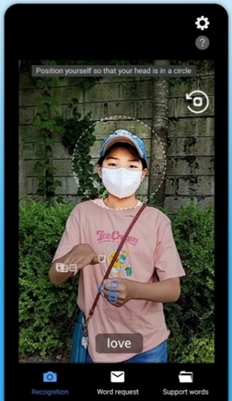
\includegraphics[width=0.25\linewidth]{figuras/ai_sign_lenguaje.png}
    \caption{Muestra de aplicación “Sign Language Translator AI”}
    \label{fig:enter-label}
\end{figure}

\subsubsection{Resumen de Funcionalidades y Características Destacadas de Aplicaciones Investigadas}

Luego de la investigación previa, se destacan las siguientes funcionalidades:
\begin{itemize}
    \item Espacio para grabar un video con indicadores de posición y luz adecuados para garantizar una captura óptima del vídeo.
    \item Modo ayuda para tutorial.
    \item Botón de compartir para difundir textos traducidos en redes sociales.
    \item Botón de agregar a favoritos la traducción realizada.
    \item Botón de reproducción de voz.
    \item Botón para calificar la traducción.
    \item Historial de videos grabados.
    \item Lista de palabras reconocibles.
\end{itemize}

Asimismo, destacan las siguientes características de diseño:
\begin{itemize}
    \item Diseño limpio e intuitivo.
    \item Paleta de colores atractiva.
    \item Botones descriptivos para mayor comprensión de su función.
\end{itemize}

% ---------------------------------------------------------------------------------------------------------------

\subsection{Investigación de la situación actual de los sordos en Guatemala}

En Guatemala, se estima que hay aproximadamente 240,000 personas sordas, lo que representa el 3\% de la población mayor de cuatro años, según datos del Instituto Nacional de Estadística (INE). Las causas de la sordera son diversas e incluyen factores genéticos, complicaciones durante el nacimiento y enfermedades infecciosas. Uno de los principales desafíos que enfrentan las personas sordas en el país es la comunicación, lo cual limita su capacidad para participar de manera equitativa en la sociedad \cite{CongresoGuatemala} \cite{GobiernoGuatemala2022}.

La lengua de señas reconocida es LENSEGUA. Las personas sordas están dispersas por todo el territorio nacional, pero se estima que la mayoría que saben LENSEGUA están concentradas principalmente en la ciudad capital. En áreas rurales con acceso limitado a la educación, como el norte de Petén, las personas sordas a menudo desarrollan sus propios sistemas de señas \cite{JoshuaProject}. 

El ámbito educativo presenta desafíos notables. A pesar de la existencia de organizaciones como la Asociación Nacional de Sordos de Guatemala, que brinda educación y otros servicios, las oportunidades educativas son escasas, especialmente en áreas rurales. Muchos estudiantes sordos deben alejarse de sus familias para acceder a opciones educativas que incluyan instrucción en lengua de señas. Un gran número de ellos ni siquiera tiene la oportunidad de acceder a una educación básica debido a la escasez de maestros capacitados en lengua de señas. Menos del 50\% recibe educación formal y las escuelas rara vez ofrecen niveles de educación secundaria. Aquellos que persiguen estudios superiores a menudo lo hacen sin la ayuda de intérpretes, lo que complica su aprendizaje y progreso académico. Esto perpetúa un ciclo de desventajas educativas y económicas, con altas tasas de desempleo y dependencia económica entre la comunidad sorda \cite{EndangeredLanguages}.

El desempleo es elevado en esta comunidad debido a las barreras comunicativas y la falta de adaptaciones adecuadas en los lugares de trabajo. La mayoría de las personas sordas vive con sus padres y están relegadas a trabajos de mano de obra básica debido a las barreras para obtener empleos mejor remunerados \cite{EndangeredLanguages}.

A pesar de estos retos, ha habido iniciativas para mejorar la inclusión de las personas sordas en Guatemala. Por ejemplo, el Benemérito Comité Pro-Ciegos y Sordos de Guatemala, en colaboración con SEGEPLAN, ha trabajado en promover la educación inclusiva y el empleo equitativo, aunque la implementación efectiva de estas políticas aún enfrenta obstáculos significativos \cite{GobiernoGuatemala2022}.

%------------------------------------------------------------------------------------------------------

\subsection{Preparación y realización de entrevistas y encuestas}

\subsubsection{Entrevista a Doctor Miguel Angel Gonzalez Palacios}

El Dr. Gonzalez, médico general con más de 25 años de experiencia, compartió sus reflexiones sobre la importancia de mejorar la comunicación con pacientes sordos. Durante la entrevista, destacó las dificultades que enfrenta en su práctica diaria, particularmente en la correcta comprensión de los síntomas y necesidades de los pacientes sordos, lo cual es fundamental para proporcionar un diagnóstico preciso y un tratamiento efectivo.

El Dr. Gonzalez expresó su entusiasmo por la iniciativa de la aplicación "Señas Chapinas", mencionando que una herramienta de este tipo podría ser revolucionaria para la práctica médica. Resaltó el potencial de la aplicación para facilitar una comunicación fluida y precisa con pacientes sordos, reduciendo los malentendidos y aumentando la calidad del cuidado médico. 

\subsubsection{Entrevista a Licenciada Claudia Barrillas}

En la entrevista con la abogada Barrillas, se abordó el contexto legal de las personas sordomudas en Guatemala, destacando la importancia de proteger sus derechos en los procedimientos judiciales. Se resaltó la necesidad de contar siempre con un intérprete de lengua de señas durante las declaraciones para asegurar una comunicación efectiva. La escasez de intérpretes, sin embargo, puede provocar demoras en los procesos legales. La Licenciada Barrillas enfatizó el valor de una aplicación de traducción de lengua de señas que podría permitir una comunicación más fluida y directa, reduciendo la dependencia de intermediarios y mejorando el acceso a la justicia para las personas sordomudas, fomentando la inclusión y la igualdad.

Se mencionaron casos donde la ausencia de intérpretes resultó en injusticias o malentendidos legales, subrayando la importancia de una comunicación clara y efectiva en el ámbito judicial. La profesional propuso que una aplicación de traducción de lengua de señas no solo facilitaría la comunicación en procesos legales, sino que también promovería una mayor autonomía para las personas sordomudas, eliminando muchas barreras que enfrentan cotidianamente.

\subsubsection{Entrevista con Profesora Carmen Lucía Guerrero}

Carmen Guerrero es profesora en la Universidad del Valle de Guatemala y forma parte del departamento de Educación para personas con necesidades especiales. Su trabajo le ha permitido adquirir conocimientos en LENSEGUA y establecer contacto directo con miembros de la comunidad sorda.

En esta entrevista se abordaron temas clave sobre la estructura y adaptación del español signado en la lengua de señas. 

La profesora Guerrero explicó que las personas que nacen sordas generalmente aprenden la lengua de señas como su primer idioma, lo cual posee una gramática y estructura propias, distintas del español hablado. Por otro lado, aquellas que pierden la audición más tarde en la vida pueden intentar adaptar su forma de hablar al español, conservando características del lenguaje oral. Este contraste muestra cómo la forma de comunicación varía significativamente entre quienes han sido sordos desde el nacimiento y quienes se han vuelto sordos posteriormente.

Uno de los desafíos discutidos fue la falta de un estándar unificado en la lengua de señas en Guatemala, lo que lleva al uso de señas específicas en regiones como Quetzaltenango. Esta variabilidad regional complica la comunicación y la educación en lengua de señas. Además, la profesora subrayó la importancia de contar con intérpretes y educadores certificados por el Ministerio de Educación para asegurar utilizar LENSEGUA “oficial”. 

También se mencionó que muchas de las señas utilizadas en Guatemala son adaptaciones de la lengua francesa, compartiendo similitudes gramaticales con este idioma. La licenciada recomendó la necesidad de investigar más sobre estas reglas gramaticales y consultar documentación específica que pueda profundizar el entendimiento y la correcta aplicación de la lengua de señas.

La conversación también resaltó la relevancia de la posición y el movimiento de las manos en la comunicación a través de señas, dado que pequeñas variaciones pueden alterar significativamente el significado de las palabras. Por ejemplo, las señas para ``hola'' y ``gracias'' son muy parecidas y pueden confundirse fácilmente. 

Finalmente, se recalcó que no siempre es posible traducir todas las palabras directamente a señas, lo que destaca la complejidad de desarrollar recursos efectivos para la comunicación en lengua de señas y la importancia de adaptar continuamente las herramientas educativas y de comunicación para satisfacer las necesidades de la comunidad sorda.


\subsubsection{Entrevista a intérprete de En-Señas Melany Cordero}

Melany Cordero, quien ejerce como intérprete y maestra de nivel medio en En-Señas, acompaña a profesoras al impartir clases y asiste en la resolución de dudas de los alumnos. Comenzó su formación en LENSEGUA en la academia y obtuvo su diploma que la acredita como intérprete.

Durante la entrevista, Melany expresó que la propuesta de la aplicación ``Señas Chapinas'' le pareció tanto útil como innovadora. Sugirió agregar elementos como juegos o retos diarios, para fomentar un aprendizaje continuo y efectivo de LENSEGUA entre los usuarios. Propuso, por ejemplo, implementar un juego de memoria o un ejercicio similar a los utilizados en exámenes, donde se presenta una palabra y los usuarios deben seleccionar la seña correcta asociada. Estas actividades no solo mantendrían el interés de los usuarios, sino que también potenciarían su capacidad de aprendizaje y retención de la lengua de señas de manera divertida y desafiante.


\subsubsection{Entrevista a Director General de En-Señas Antonio Barrientos}

El señor Barrientos desarrolló un interés por la lengua de señas inspirado por su madre, quien también la aprendió y frecuentaba a la comunidad sorda. Motivado por su deseo de entender las conversaciones de este grupo, el señor se sumergió en el estudio de la lengua de señas y actualmente es intérprete de nivel avanzado y director general de la institución ``En-Señas''.

Durante la entrevista, el Director señaló que una de las principales complicaciones con la aplicación ``Señas Chapinas'' es la falta de un estándar uniforme para LENSEGUA. Explicó que existen variaciones significativas en el uso de señas entre los diferentes departamentos de Guatemala, e incluso entre distintas instituciones educativas, lo que puede complicar la precisión de las traducciones. Esta diversidad se debe a la ausencia de una entidad reguladora que estandarice las señas y certifique quiénes están calificados para enseñar LENSEGUA. No obstante, actualmente hay esfuerzos para lograr esta estandarización.

El Director también destacó la escasez de materiales e información en línea sobre LENSEGUA, así como las deficiencias legislativas que, aunque reconocen la lengua de señas, no establecen un marco regulatorio suficiente para su enseñanza y promoción.

En cuanto a la comunidad sorda, mencionó que existen cuatro categorías distintas: personas que utilizan señas caseras y no interactúan con LENSEGUA, aquellas que aprenden a leer los labios, los usuarios de LENSEGUA, y los bilingües, que combinan la lectura de labios con el uso de la lengua de señas.

Finalmente, el Director Barrientos abordó el alto índice de analfabetismo en la comunidad sorda, atribuyéndolo a las diferencias en el nivel de apoyo que reciben desde la infancia. Mientras algunas familias fomentan el aprendizaje de la lengua de señas y la terapia del habla desde temprana edad, otras dejan a las personas sordas sin el soporte necesario para su desarrollo educativo.

\subsubsection{Entrevista a persona sorda hipoacúsica y maestra de En-Señas Gabriela Velázquez}
La señora Velázquez, una maestra de 59 años de En-Señas y persona sorda hipoacúsica, nació en Guatemala y actualmente enseña LENSEGUA tanto a personas sordas como oyentes. Está casada con una persona sorda profunda. 

Durante su infancia, la señora Gabriela relata que era común que las personas sordas fueran obligadas a aprender a vocalizar mediante terapia del habla y lectura de labios, en lugar de aprender LENSEGUA. No fue hasta la edad adulta que aprendió este medio de comuniación, convirtiéndose en bilingüe, lo cual marcó una mejora significativa en su comprensión lectora y en la ampliación de su vocabulario. Aunque la profesora puede leer labios, encuentra este método desafiante y prefiere comunicarse usando LENSEGUA, lo que le resulta más cómodo y eficaz. Ella señala que, para las personas sordas profundas, vocalizar puede ser aún más difícil, por lo que generalmente dependen más de LENSEGUA, lo que a menudo complica su comprensión del español escrito.

Sobre la aplicación ``Señas Chapinas'', la profesora Gabriela considera que sería útil para usuarios de LENSEGUA y destacó la importancia de que la aplicación ofrezca tanto la traducción palabra por palabra como la oración completa en español. Esto ayudaría a los usuarios a verificar la traducción de las señas y facilitaría el aprendizaje de la gramática en español. La profesora Velázquez y sus conocidos frecuentemente utilizan \textit{ChatGPT}, escribiendo en gramática de LENSEGUA para que el sistema lo traduzca al español, lo que les ayuda a confirmar que están escribiendo correctamente.

Ella menciona que ``Señas Chapinas'' la usaría principalmente en situaciones donde no hay un intérprete presente, como visitas al médico, reuniones con abogados, testimonios en corte, emergencias y reuniones familiares. Menciona que en Estados Unidos existe un servicio de intérpretes que funciona como un \textit{call center}, donde se ofrece traducción a lengua de señas de forma simultanea, y sugiere que la aplicación podría replicar este servicio en Guatemala, ofreciendo traducciones de LENSEGUA a texto o voz.

Además, destacó que la aplicación podría contribuir a reducir el analfabetismo entre los sordos, permitiéndoles aprender al grabar videos en LENSEGUA y ver las traducciones al español. 

En el contexto de las aplicaciones móviles, se destacó que las personas sordas utilizan continuamente sus teléfonos, especialmente para acceder a redes sociales y aplicaciones de videollamadas. Estas herramientas les permiten interactuar con amigos, familiares y conocidos de manera más dinámica. Continua relatando que antes de la llegada de los teléfonos inteligentes, la comunicación era notablemente más complicada; sin embargo, hoy en día, la tecnología facilita significativamente el aprendizaje de LENSEGUA en línea y mejora la comunicación general. 

La profesora Velázquez prefiere las aplicaciones que requieren poco texto y presentan interfaces de usuario simples y directas, ya que son más fáciles de utilizar. Además, comentó que las aplicaciones lentas y complejas resultan menos atractivas para los ella y sus conocidos.

Para la profesora, un aspecto crucial de la aplicación ``Señas Chapinas'' es que reconozca las diversas variantes y modismos presentes en LENSEGUA. Este detalle es fundamental para asegurar que la aplicación sea verdaderamente inclusiva y efectiva para todos los usuarios de la lengua de señas guatemalteca, reflejando las diferencias regionales y de estilo que caracterizan su uso cotidiano.

Además, Gabriela Velázquez espera que la aplicación le sirva como una herramienta para enriquecer su vocabulario y gramática en español. Al incorporar funciones que permitan aprender y practicar español, la aplicación no solo serviría para traducir de LENSEGUA a español, sino que también funcionaría como un recurso educativo, apoyando el desarrollo lingüístico integral de sus usuarios.


\begin{figure} [H]
    \centering
    \includegraphics[width=0.5\linewidth]{figuras/entrevista.png}
    \caption{Entrevista En-Señas}
    \label{fig:enter-label}
\end{figure}

\subsubsection{Primera encuesta Señas Chapinas}

La primera encuesta para el proyecto ``Señas Chapinas'' consta de varias secciones diseñadas para recopilar información y opiniones sobre la necesidad de superar las barreras de comunicación en Guatemala a través de una aplicación móvil.

La primera sección recopila datos demográficos como edad, género, lugar de nacimiento, profesión y si el encuestado presenta dificultades auditivas o del habla.

La segunda sección está bifurcada según si los encuestados son sordos o no. Para los que no son sordos, se investiga si conocen a alguien con dificultades auditivas y cómo han utilizado tecnología de asistencia para comunicarse con ellos. Además, se indaga sobre los desafíos percibidos para estas personas y en qué contextos una aplicación de traducción de señas sería beneficiosa. Para los encuestados sordos, se solicita que compartan sus experiencias con otras herramientas de asistencia, desafíos específicos enfrentados en Guatemala, situaciones de frustración al comunicarse, y cómo una aplicación podría mejorar su comunicación diaria.

La tercera sección evalúa la percepción sobre la utilidad de la aplicación para convertir la lengua de señas a texto o voz, recogiendo expectativas y características deseadas. Además, se piden sugerencias sobre funcionalidades adicionales y posibles contextos de uso.

Los resultados de esta primera encuesta no fueron los esperados. Los participantes sordos de nacimiento encontraron las preguntas demasiado complejas, atribuyéndolo a las diferencias gramaticales en su lenguaje. Esto llevó a la necesidad de desarrollar una encuesta específica para personas oyentes y planificar entrevistas con intérpretes para personas sordas.


\subsubsection{Segunda encuesta Señas Chapinas}

Como resultado de los comentarios y sugerencias recopilados en la primera encuesta, se desarrolló una segunda encuesta dirigida específicamente a personas oyentes (ver Anexo~\ref{anexo:encuesta_oyentes}). Esta encuesta se dirige a individuos sin conocimiento previo de LENSEGUA, a aquellos que regularmente interactúan con personas sordas, y a intérpretes. 

La sección inicial de la encuesta proporciona un análisis demográfico de los participantes. Los resultados muestran que la mayoría de los encuestados son hombres. Además, el grupo de edad más representado está entre los 18 y 24 años. 

\begin{figure} [H]
    \centering
    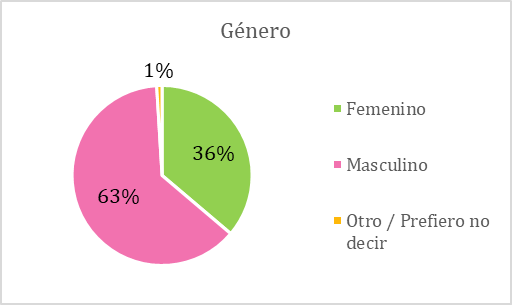
\includegraphics[width=0.5\linewidth]{figuras/encuesta_genero.png}
    \caption{Género Encuesta 2}
    \label{fig:enter-label}
\end{figure}

\begin{figure} [H]
    \centering
    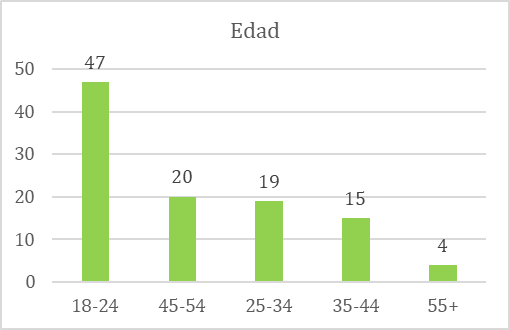
\includegraphics[width=0.5\linewidth]{figuras/encuesta_edad.png}
    \caption{Edad Encuesta 2}
    \label{fig:enter-label}
\end{figure}

La siguiente sección de la encuesta está destinada a explorar el conocimiento y la experiencia con la lengua de señas. Alrededor del 40\% de los encuestados indica conocer a alguien sordo, lo que destaca una conexión significativa con la comunidad sorda. Adicionalmente, cerca del 70\% percibe la aplicación como relevante, mostrando un interés considerable en la herramienta propuesta. Sin embargo, es notable que aproximadamente el 70\% de los participantes no están familiarizados con LENSEGUA, lo cual es entendible considerando que su reconocimiento oficial data de hace solo cuatro años. \cite{CongresoGuatemala2020}. 

\begin{figure} [H]
    \centering
    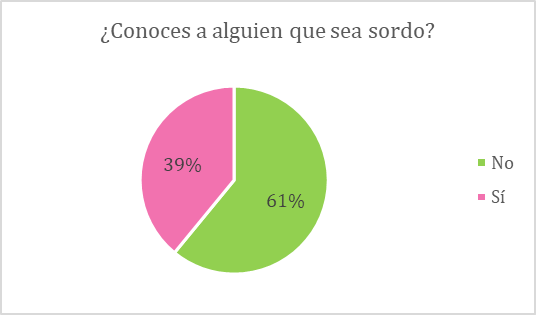
\includegraphics[width=0.5\linewidth]{figuras/conocimientoSordaEncuesta.png}
    \caption{Conocimiento Persona Sorda Encuesta 2}
    \label{fig:enter-label}
\end{figure}

\begin{figure} [H]
    \centering
    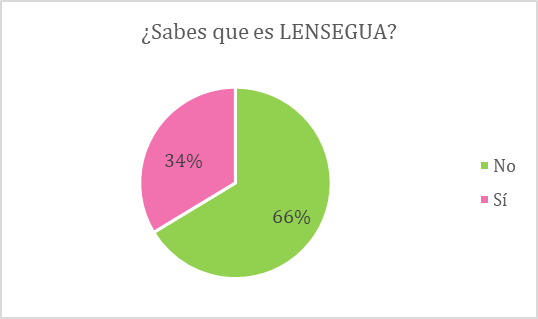
\includegraphics[width=0.5\linewidth]
    {figuras/conoimiento_lensegua.png}
    \caption{Conocimiento LENSEGUA Encuesta 2}

\end{figure}

\begin{figure} [H]
    \centering
    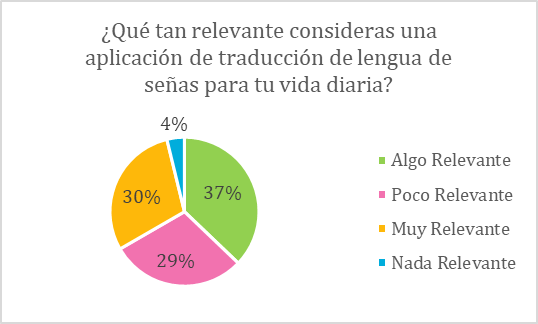
\includegraphics[width=0.5\linewidth]{figuras/relevancia_app.png}
    \caption{ Relevancia de la Aplicación Encuesta 2}
    \label{fig:enter-label}
\end{figure}


Además, se realizó un análisis comparativo entre los encuestados que conocen a personas sordas y su percepción de la relevancia de la aplicación. Los resultados muestran que aquellos familiarizados con la comunidad sorda tienden a valorar más la aplicación en comparación con quienes no tienen contacto directo con personas sordas. Este hallazgo sugiere que la experiencia personal y el conocimiento de los retos enfrentados por las personas sordas pueden influir significativamente en la percepción de la utilidad de herramientas tecnológicas como un traductor de lengua de señas.

\begin{figure} [H]
    \centering
    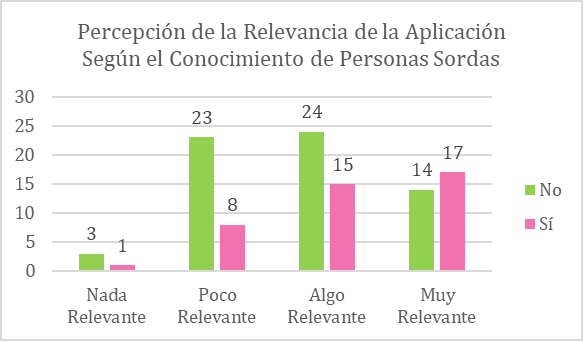
\includegraphics[width=0.5\linewidth]{figuras/relevancia_app_conocidos.png}
    \caption{Relevancia de la Aplicación para Personas con Conocidos Sordos Encuesta 2}
    \label{fig:enter-label}
\end{figure}

Para comprender mejor las estrategias de comunicación que las personas emplearían con individuos sordos, se les preguntó a los encuestados sobre sus métodos preferidos. La mayoría, casi el 60\%, optaría por el uso de mensajes escritos, mientras que un 18\% indicó que señalarían objetos para hacerse entender. Solo un 9\% consideraría usar LENSEGUA. Es notable que solo una minoría, aproximadamente el 10\%, expresó no saber cómo comunicarse, reflejando así el interés general por explorar formas de interacción. Algunos participantes también mencionaron la lectura de labios como alternativa, aunque es importante destacar que no todos los sordos tienen la capacidad de leer los labios.

Para profundizar en el entendimiento que tienen las personas sobre los desafíos que enfrentan los sordos, se les preguntó cuáles consideraban que eran las mayores dificultades para esta comunidad. Las respuestas revelaron una conciencia sobre la falta de inclusión y herramientas adecuadas para personas sordas, destacando cómo muchas infraestructuras y servicios en Guatemala están diseñados principalmente para oyentes. Además, se mencionaron problemas como segregación y discriminación en la sociedad, así como la escasez de enseñanza de la lengua de señas.

Entre las preocupaciones más citadas también estuvieron la ausencia de sistemas de alerta para sordos en situaciones de emergencia y barreras significativas en comunicación. Los encuestados resaltaron la existencia de prejuicios y la dificultad en la realización de tareas cotidianas y trámites, lo que contribuye al aislamiento social y a la exclusión. Esta variedad de respuestas ilustra la complejidad de los desafíos a los que se enfrentan los sordos. 

La siguiente sección de la encuesta se centró en la aplicación "Señas Chapinas", explorando las motivaciones principales para usar una herramienta de traducción de lengua de señas. Destacablemente, el 60\% de los participantes indicaron la curiosidad personal como su principal motivación. Casi la mitad de los encuestados mencionaron la comunicación con amigos o familiares sordos como un factor importante, subrayando la relevancia personal y social de la aplicación. Además, cerca del 40\% expresaron que utilizarían la aplicación para actividades voluntarias, lo que refleja su potencial utilidad en entornos de servicio comunitario. Un pequeño porcentaje citó los requerimientos laborales como motivo, sugiriendo su aplicación en contextos profesionales donde la interacción con personas sordas es frecuente. Otras respuestas revelaron usos más específicos y personales, evidenciando la diversidad de situaciones en las que los usuarios anticipan la utilidad de la aplicación.

También se indagó en que situaciones los usuarios desean emplear la aplicación ``Señas Chapinas''. Predominantemente, las actividades sociales representan el escenario más popular, con un 78.6\% de los encuestados seleccionándolo. Esto es seguido por el voluntariado y la educación, con un 67.6\% y un 49\%, respectivamente. El trabajo también es una situación comúnmente identificada, con un 40.2\% de los encuestados expresando la necesidad de utilizar la aplicación en este contexto. Estos resultados indican una fuerte preferencia por utilizar la aplicación en contextos grupales y de interacción, lo que subraya la importancia de la aplicación en facilitar la comunicación en una variedad de entornos cotidianos y profesionales.

La última sección pregunta las características más importantes en una aplicación móvil. En la última sección de la encuesta, los encuestados identificaron las características más importantes en una aplicación móvil. La facilidad de uso fue la más destacada, valorada por el 98.1\% de los participantes, seguida por la velocidad y rendimiento (61.9\%), funciones de accesibilidad (54.3\%), y diseño atractivo (46.7\%). Esto resalta la importancia de una interfaz intuitiva, un rendimiento eficiente, accesibilidad adecuada, y un diseño visualmente atractivo para los usuarios de esta aplicación. 

Finalmente se dio espacio para comentarios adicionales. En la sección final de la encuesta se exploraron las características esenciales para una aplicación de traducción de lengua de señas. La facilidad de uso fue una de las características más mencionadas, destacando su importancia para una adopción rápida por parte de los usuarios. Muchos encuestados valoraron también la velocidad y la precisión de la traducción, subrayando la necesidad de interacciones fluidas y sin errores. Algunas otras sugerencias fueron mencionadas, pero serán tomadas en cuenta para futuras mejoras, pues no están dentro del alcance del presente proyecto. 

\subsubsection{Entrevista Colectiva a miembros de En-Señas}

Con un conocimiento más profundo de las necesidades de las personas sordas, sus familias y conocidos, así como del nivel de conciencia de la población guatemalteca sobre LENSEGUA, se llevó a cabo una última entrevista colectiva con miembros de Enseñas. Durante esta sesión, se presentó el concepto de la aplicación y se recogieron sus opiniones. Los comentarios más destacados incluyeron:

\begin{itemize}
    \item \textbf{Uso de Redes Sociales:} Las personas sordas frecuentan plataformas sociales, especialmente TikTok, por su facilidad e intuitividad de uso.
    
    \item \textbf{Funcionalidades Educativas}: Se sugirió que la aplicación también debería facilitar el aprendizaje de LENSEGUA en Guatemala, incorporando juegos interactivos que fomenten la participación activa.
    
    \item \textbf{Diseño Atractivo y Profesional}: La aplicación debe ser visualmente llamativa sin sacrificar su seriedad, generando confianza en que se trata de una herramienta fiable y efectiva.
    
    \item \textbf{Futuras Expansiones}: Se anticipa que, eventualmente, la aplicación podrá traducir del español a LENSEGUA.
    
    \item \textbf{Vocabulario Adecuado}: En las primeras fases, el vocabulario debe ser simple y cotidiano, incluyendo términos de uso frecuente y frases de emergencia.
    
    \item \textbf{Reporte de Errores:} Es crucial que las traducciones incorrectas puedan ser reportadas fácilmente por los usuarios sordos para que el equipo detrás de la aplicación pueda investigar y resolver cualquier inconveniente.
    
    \item \textbf{Guardado de Favoritos:} Los usuarios expresaron el deseo de poder guardar videos de frases en LENSEGUA que utilizan regularmente, para acceder a ellos de manera rápida y sencilla.
    
    \item \textbf{Flexibilidad de Grabación}: La aplicación debe permitir grabaciones tanto con la cámara frontal como con la trasera, facilitando la captura de auto-grabaciones o de terceros.
    
    \item \textbf{Accesibilidad del Nombre}: El nombre de la aplicación debe ser fácilmente representable en señas, asegurando su accesibilidad y reconocimiento dentro de la comunidad sorda.
    
\end{itemize}

Estos valiosos comentarios guiaran la próxima fase de desarrollo para asegurar que la aplicación no solo cumpla con las expectativas de la comunidad sorda sino que también sirva como un puente cultural y educativo.


\begin{figure} [H]
    \centering
    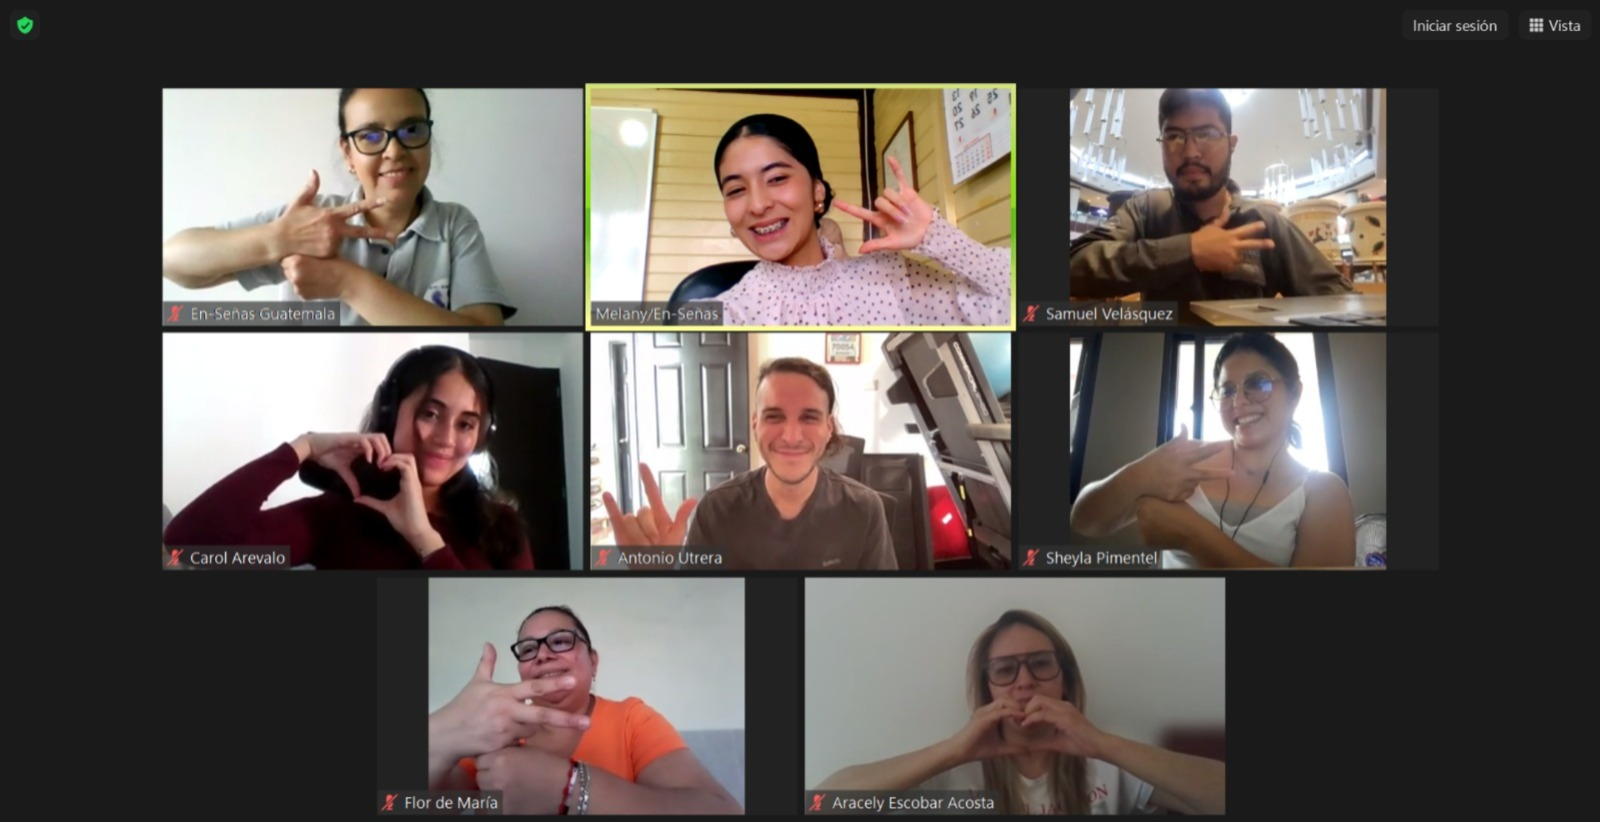
\includegraphics[width=0.75\linewidth]{figuras/entrevista_colectiva.png}
    \caption{Entrevista colectiva En-Señas}
    \label{fig:enter-label}
\end{figure}


%-------------------------------------------------------------------------------------------------------------------------------

\subsection{Colaboraciones}

Para profundizar en la comprensión de las necesidades tanto de las personas sordas como de aquellas que desean comunicarse con ellas, se decidió colaborar con varias entidades guatemaltecas dedicadas a mejorar la calidad de vida de este grupo.

En primer lugar, se participó en clases de Lengua de Señas Guatemalteca (LENSEGUA) ofrecidas por En-Señas. Esta formación permitió comprender mejor la gramática y el contexto cultural de esta lengua, elementos fundamentales para garantizar una comunicación efectiva y respetuosa.

Asimismo, la empresa ASEDES colaboró proporcionando apoyo en la realización de entrevistas y en otras actividades necesarias para el desarrollo de los diversos módulos del proyecto. Esta colaboración fue vital para asegurar que el diseño de la aplicación sea inclusivo y práctico para los usuarios.

Finalmente, la ONG Sordos Latinos de Guatemala estuvo brindando asistencia invaluable mediante el suministro de información y recomendaciones especializadas. Además, facilito entrevistas y otros recursos esenciales que enriquecieron el entendimiento y ayudaron a ajustar el proyecto para entender mejor las necesidades de la comunidad sorda en Guatemala.

%======================================================================================================
\section{DESARROLLO DE INTERFAZ Y EXPERIENCIA DE USUARIO}

\subsection{Creación de Diagrama de Afinidad}

En el desarrollo de la experiencia del usuario (UX), los diagramas de afinidad juegan un papel crucial, ya que permiten organizar y sintetizar grandes volúmenes de datos e ideas de manera visual y estructurada. Este método es especialmente valioso durante las fases iniciales de desarrollo de un proyecto, donde el entendimiento claro y la definición del problema son esenciales \cite{Maze2024}.

El proceso comienza con una lluvia de ideas, donde se generan y recopilan múltiples puntos de vista y datos sobre las necesidades y problemas de los usuarios. Esta fase es crítica, ya que establece la base de información que influirá en todas las decisiones de diseño y desarrollo subsiguientes \cite{Maze2024}.

La lluvia de ideas para Señas Chapinas organiza conceptos clave en categorías codificadas por colores, facilitando la identificación y el análisis de diversas áreas del proyecto:

\begin{itemize}
    \item \textbf{Naranja:} Define el público objetivo de la aplicación.
    \item \textbf{Amarillo:} Enumera los objetivos y metas que la aplicación pretende alcanzar.
    \item \textbf{Azul:} Destaca información crucial necesaria para el desarrollo de la aplicación.
    \item \textbf{Rojo:} Señala los problemas y desafíos que la aplicación busca resolver.
    \item \textbf{Verde:} Detalla las características y funcionalidades esperadas de la aplicación.
\end{itemize}

Este enfoque visual no solo ayuda a estructurar el proceso de planificación, sino que también asegura que todos los aspectos relevantes sean considerados, apoyando una toma de decisiones informada y alineada con las necesidades de los usuarios.

\begin{figure} [H]
    \centering
    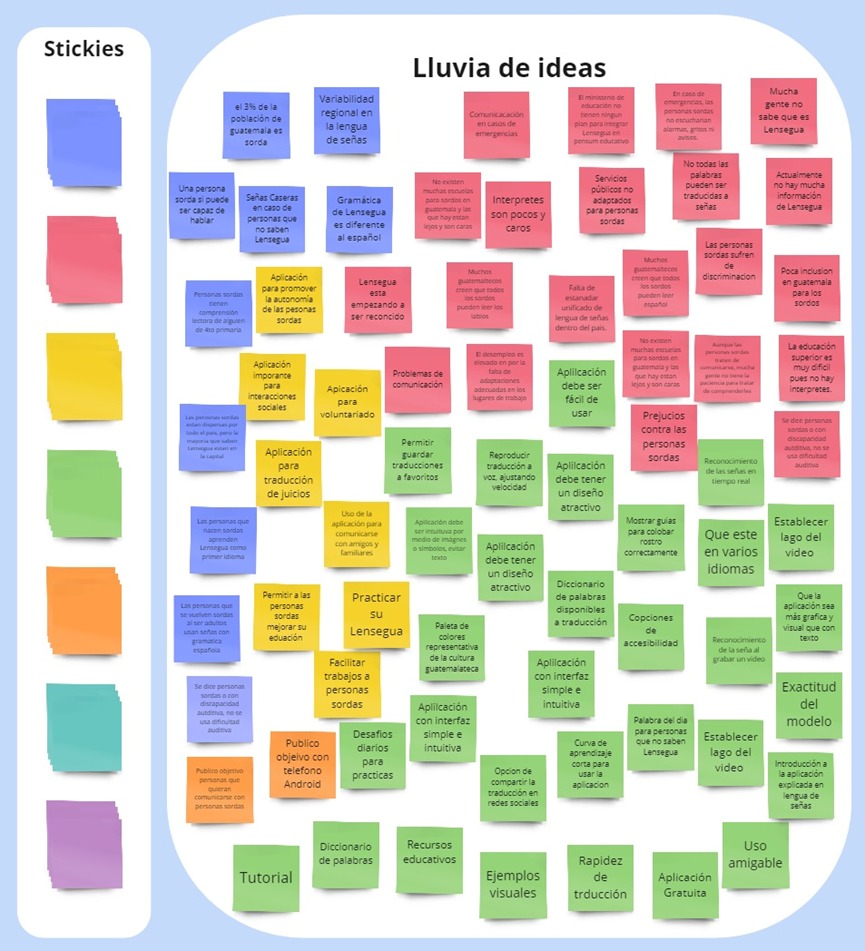
\includegraphics[width=0.75\linewidth]{figuras/lluevia_diagrama_afinidad.png}
    \caption{Lluvia de Ideas para Diagrama de Afinidad}
    \label{fig:enter-label}
\end{figure}

Posteriormente, se agrupan las ideas similares con el objetivo de identificar patrones y temas comunes. Este proceso implica organizar los datos recolectados durante la lluvia de ideas en categorías que reflejen conexiones y tendencias subyacentes. Al hacer esto, se pueden observar relaciones entre las diferentes opiniones y necesidades, facilitando la creación de soluciones más coherentes y efectivas que aborden los desafíos identificados de manera integral. Este método no solo ayuda a clarificar el alcance del proyecto, sino que también proporciona una base sólida para las decisiones de diseño y desarrollo subsiguientes, asegurando que se consideren todas las perspectivas relevantes.

\begin{figure} [H]
    \centering
    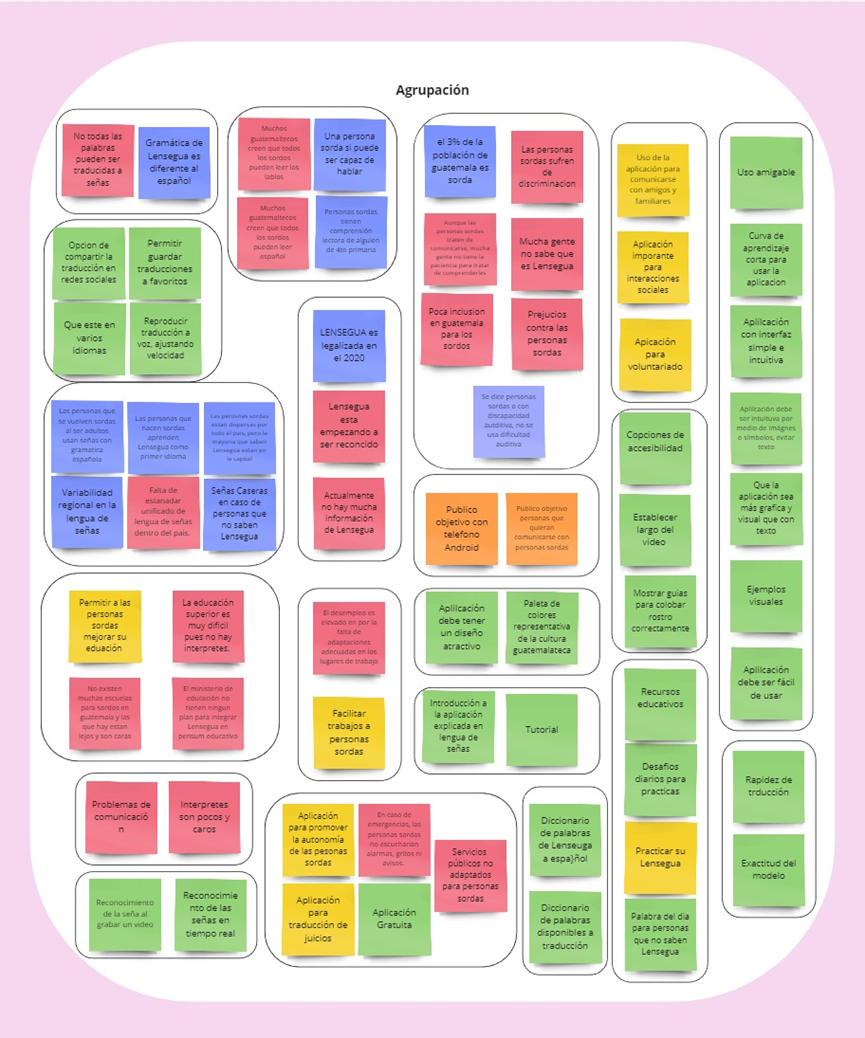
\includegraphics[width=0.75\linewidth]{figuras/agrupacion_diagrama_afinidad.png}
    \caption{Agrupación de Ideas para Diagrama de Afinidad}
    \label{fig:enter-label}
\end{figure}

Finalmente, se realiza el diagrama de afinidad, que sintetiza todas las ideas recolectadas y categorizadas previamente. Este diagrama visual, organizado por colores, facilita la interpretación de la información y permite una evaluación clara de cómo cada aspecto del proyecto interacciona y contribuye al objetivo global. Al agrupar las ideas en distintas categorías, como Público Objetivo, Problemas a Resolver, Objetivos, Escenarios de Uso, Funcionalidades a Desarrollar y Características de la Aplicación, se destaca la interconexión entre los requisitos del usuario y las soluciones propuestas.

\begin{figure} [H]
    \centering
    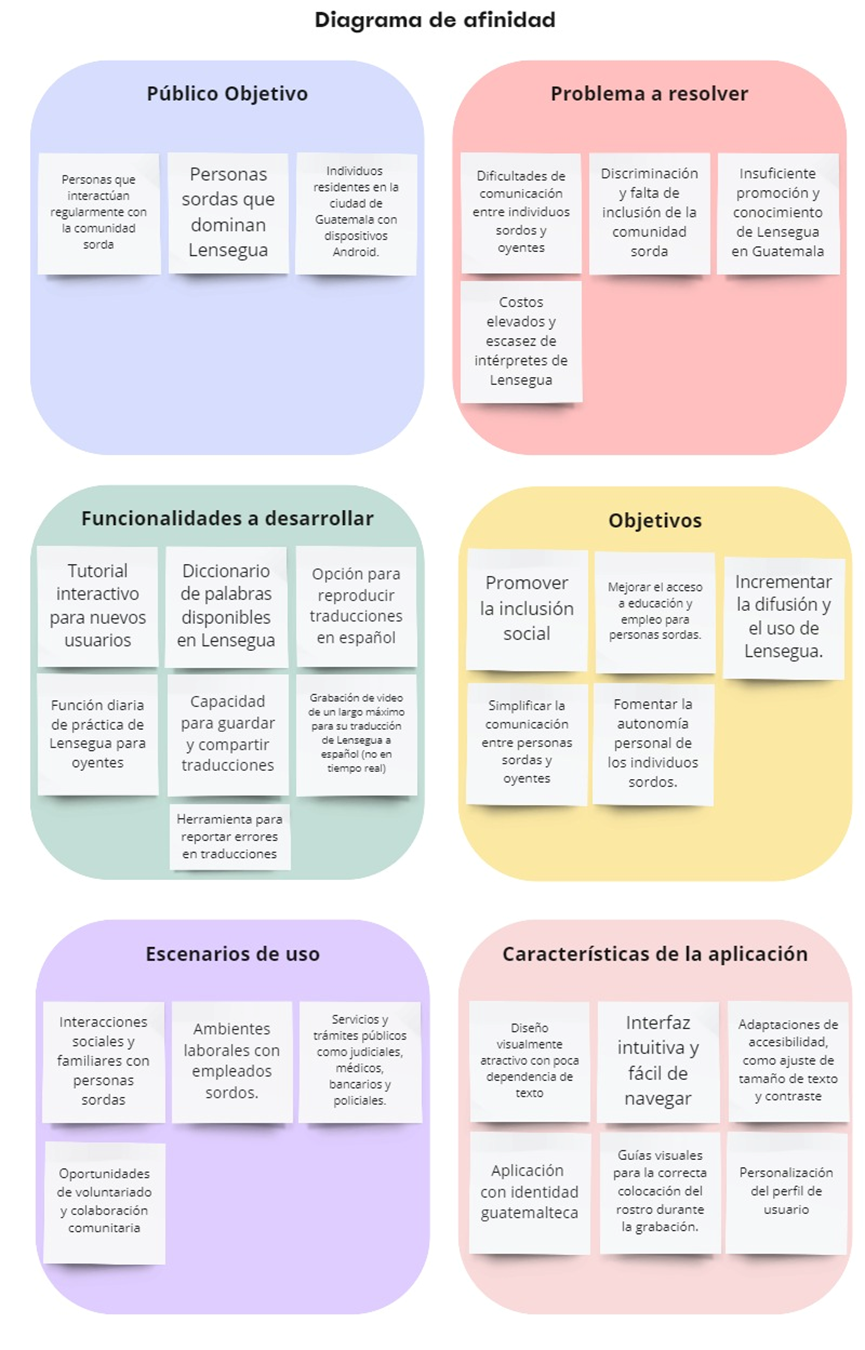
\includegraphics[width=1\linewidth]{figuras/diagrama_afinidad.png}
    \caption{Diagrama de Afinidad}
    \label{fig:enter-label}
\end{figure}

\begin{enumerate}

    \item \textbf{Público Objetivo} 
    Define a las personas que se beneficiarán directamente de la aplicación, incluyendo a aquellos que interactúan regularmente con la comunidad sorda y a las personas sordas que dominan LENSEGUA.
    \begin{itemize}
        \item Personas que interactúan regularmente con la comunidad sorda
        \item Personas sordas que dominan LENSEGUA
        \item Individuos residentes en la ciudad de Guatemala con dispositivos Android
    \end{itemize}
    
    \item \textbf{Problema a Resolver} 
    Identifica los principales desafíos que enfrenta la comunidad sorda y que la aplicación busca abordar, como las dificultades de comunicación entre sordos y oyentes, la discriminación y los altos costos de los servicios de interpretación.
    \begin{itemize}
        \item Dificultades de comunicación entre individuos sordos y oyentes
        \item Discriminación y falta de inclusión de la comunidad sorda
        \item Costos elevados y escasez de intérpretes de LENSEGUA
    \end{itemize}
    
    \item \textbf{Funcionalidades a Desarrollar} 
    Describe las características específicas que tendrá la aplicación. 
    \begin{itemize}
        \item Diccionario de palabras disponibles en LENSEGUA
        \item Función diaria de práctica de LENSEGUA para oyentes
        \item Capacidad para guardar y compartir traducciones
        \item Herramienta para reportar errores en traducciones
        \item Opción para reproducir traducciones en español
        \item Grabación de video de un largo máximo para su traducción de LENSEGUA a español (no en tiempo real)
    \end{itemize}
    
    \item \textbf{Objetivos} 
    Detalla los objetivos principales de la aplicación, como promover la inclusión social, mejorar el acceso a la educación y empleo para personas sordas, y simplificar la comunicación entre sordos y oyentes.
    \begin{itemize}
        \item Promover la inclusión social
        \item Simplificar la comunicación entre personas sordas y oyentes
        \item Mejorar el acceso a educación y empleo para personas sordas
        \item Fomentar la autonomía personal de los individuos sordos
        \item Incrementar la difusión y el uso de LENSEGUA
    \end{itemize}
    
    \item \textbf{Escenarios de Uso} 
    Enumera los diferentes contextos en los que la aplicación podría ser utilizada, incluyendo interacciones sociales, ambientes laborales, y servicios públicos como trámites médicos, bancarios y policiales.
    \begin{itemize}
        \item Interacciones sociales y familiares con personas sordas
        \item Ambientes laborales con empleados sordos
        \item Servicios y trámites públicos como judiciales, médicos, bancarios y policiales
        \item Oportunidades de voluntariado y colaboración comunitaria
    \end{itemize}
    
    \item \textbf{Características de la Aplicación} 
    Resalta aspectos del diseño y la usabilidad de la aplicación, tales como su interfaz intuitiva, el diseño visual con poca dependencia de texto y adaptaciones para accesibilidad, entre otros.
    \begin{itemize}
        \item Diseño visualmente atractivo con poca dependencia de texto
        \item Interfaz intuitiva y fácil de navegar
        \item Aplicación con identidad guatemalteca
        \item Guías visuales para la correcta colocación del rostro durante la grabación
        \item Personalización del perfil de usuario
    \end{itemize}
\end{enumerate}


\subsection{Creación de Personas}

Como parte del proceso de diseño, se han definido seis personas que representan a los usuarios finales a quienes se dirige la aplicación. 

\begin{figure} [H]
    \centering
    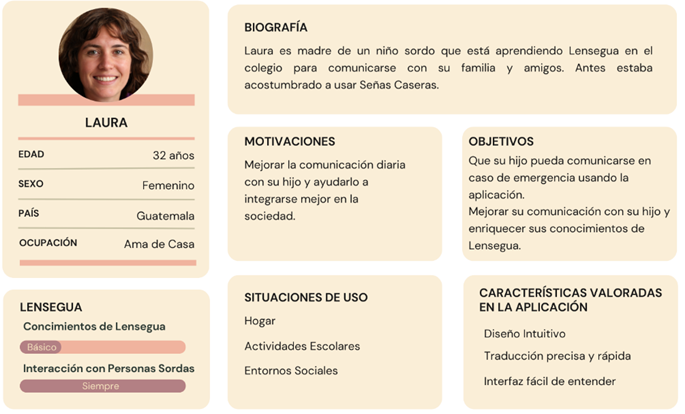
\includegraphics[width=0.8\linewidth]{figuras/persona_laura.png}
    \caption{Persona 1 - Laura}
    \label{fig:enter-label}
\end{figure}

\begin{figure} [H]
    \centering
    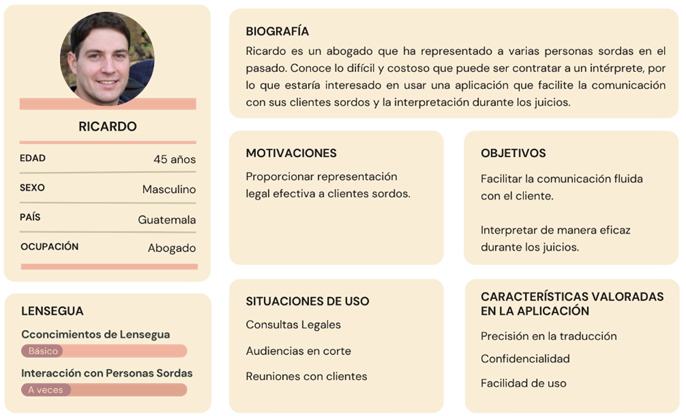
\includegraphics[width=0.8\linewidth]{figuras/ricardo_persona.png}
    \caption{Persona 2 - Ricardo}
    \label{fig:enter-label}
\end{figure}

\begin{figure} [H]
    \centering
    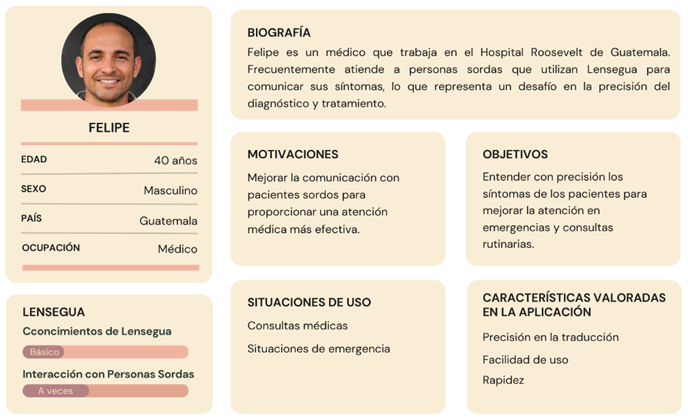
\includegraphics[width=0.8\linewidth]{figuras/felipe_persona.png}
    \caption{Persona 3 - Felipe}
    \label{fig:enter-label}
\end{figure}

\begin{figure} [H]
    \centering
    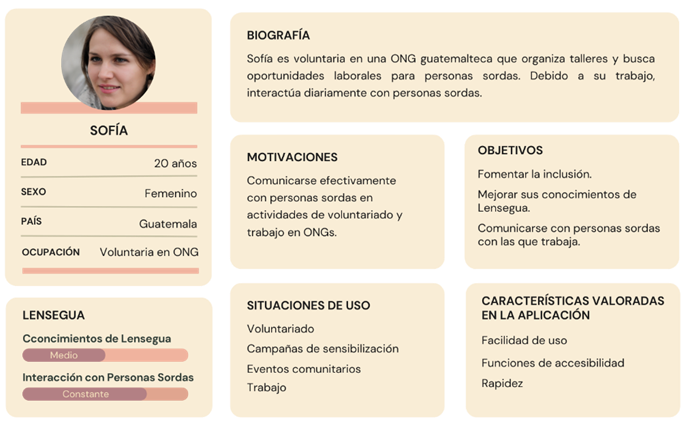
\includegraphics[width=0.8\linewidth]{figuras/sofia_persona.png}
    \caption{Persona 4 - Sofia}
    \label{fig:enter-label}
\end{figure}

\begin{figure}[H]
    \centering
    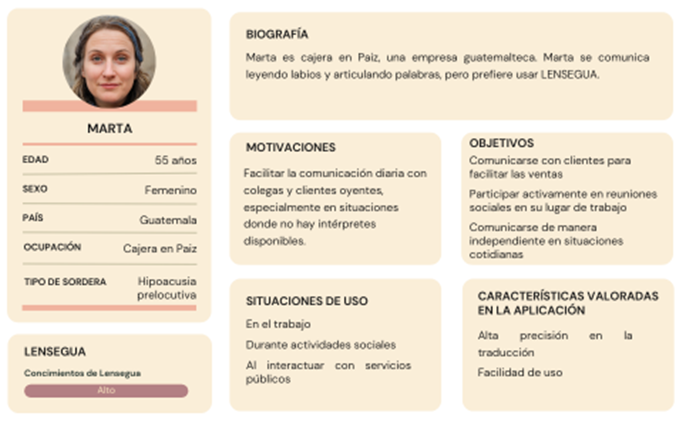
\includegraphics[width=0.8\linewidth]{figuras/marta_persona.png}
    \caption{Persona 5 - Marta}
    \label{fig:enter-label}
\end{figure}

\begin{figure} [H]
    \centering
    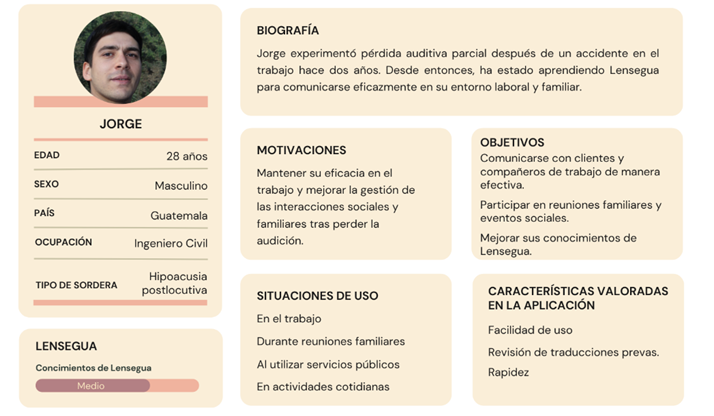
\includegraphics[width=0.8\linewidth]{figuras/jorge_persona.png}
    \caption{Persona 6 - Jorge}
    \label{fig:enter-label}
\end{figure}

% -----------------------------------------------------------------------------------------


\subsection{Creación de Mapas de Empatía}

Complementando las Personas creadas con anterioridad, se procede a crear su Mapa de Empatía respectivo para profundizar en las necesidades de los usuarios. 

\begin{figure} [H]
    \centering
    
\includegraphics[width=0.9\linewidth]{figuras/mapa_empatia_laura.png}
    \caption{Mapa de Empatía - Laura}
    \label{fig:enter-label}
\end{figure}

\begin{figure} [H]
    \centering
    
\includegraphics[width=0.9\linewidth]{figuras/mapa_empatia_ricardo.png}
    \caption{Mapa de Empatía - Ricado}
    \label{fig:enter-label}
\end{figure}

\begin{figure} [H]
    \centering
    
\includegraphics[width=0.9\linewidth]{figuras/mapa_empatia_felipe.png}
    \caption{Mapa de Empatía - Felipe}
    \label{fig:enter-label}
\end{figure}

\begin{figure} [H]
    \centering
    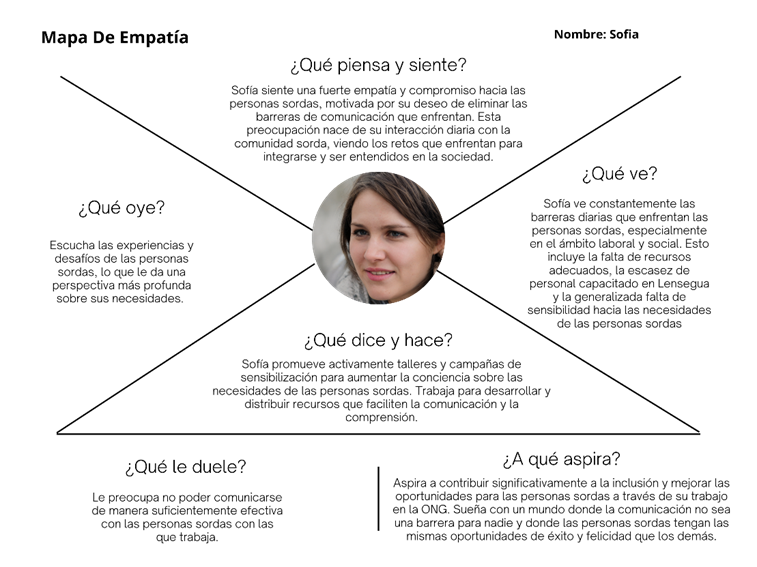
\includegraphics[width=0.9\linewidth]{figuras/mapa_empatia_sofia.png}
    \caption{Mapa de Empatía - Sofia}
    \label{fig:enter-label}
\end{figure}


\begin{figure} [H]
    \centering
    
\includegraphics[width=0.9\linewidth]{figuras/mapa_empatia_marta.png}
    \caption{Mapa de Empatía - Marta}
    \label{fig:enter-label}
\end{figure}


\begin{figure} [H]
    \centering
    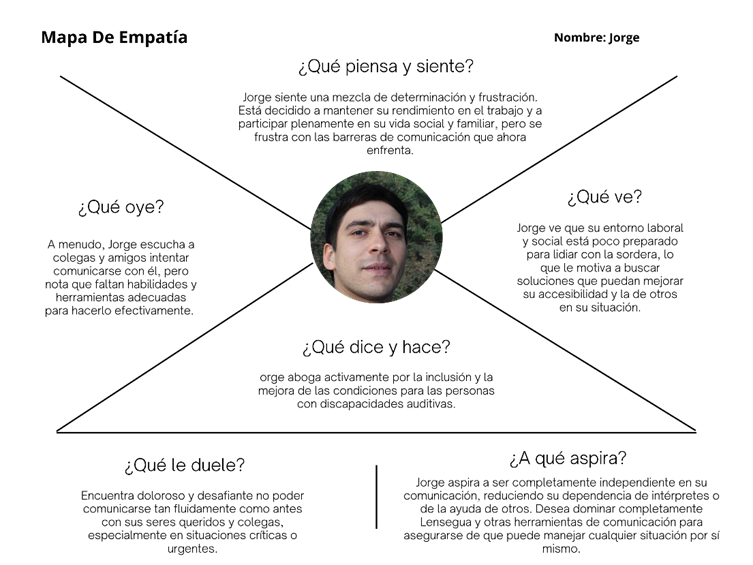
\includegraphics[width=0.9\linewidth]{figuras/mapa_empatia_jorge.png}
    \caption{Mapa de Empatía - Jorge}
    \label{fig:enter-label}
\end{figure}

% -----------------------------------------------------------------------------------------

\subsection{Planteamiento del Problema}

Inicialmente se usa Los Seis Sombreros Para Pensar, una técnica de pensamiento desarrollada por Edward de Bono en los años 80, que busca facilitar de manera creativa la resolución y el análisis de problemas desde distintos puntos de vista o perspectivas. Cada ``sombrero'' representa una dirección diferente del pensamiento y se identifica con un color específico \cite{Santos2024}.

\begin{figure} [H]
    \centering
    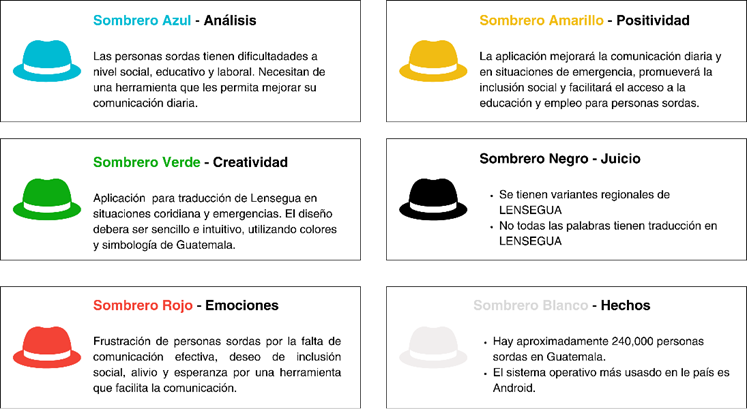
\includegraphics[width=0.8\linewidth]{figuras/sombreros.png}
    \caption{Sombreros para Pensar}
    \label{fig:enter-label}
\end{figure}


Posteriormente, se sigue el modelo W5H1 para realizar el planteamiento del problema, el cual busca ver las ideas desde varias perspectivas con el objetivo de comprender en profundidad una situación concreta \cite{Artigas2017}.

\begin{figure} [H]
    \centering
    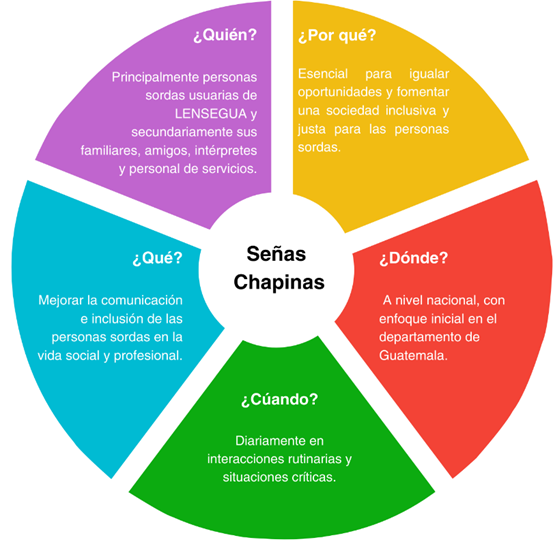
\includegraphics[width=0.6\linewidth]{figuras/w5h1.png}
    \caption{Planteamiento del Problema Señas Chapinas}
    \label{fig:enter-label}
\end{figure}

\begin{enumerate}
    \item \textbf{¿Quién?}
    \begin{enumerate}
        \item \textbf{¿A quién afecta el problema?} \\
        Afecta principalmente a personas sordas que utilizan la Lengua de Señas Guatemalteca (LENSEGUA), quienes enfrentan barreras de comunicación cotidianas.
        \item \textbf{¿Quiénes son los usuarios primarios y secundarios?}
        \begin{itemize}
            \item \textbf{Usuarios primarios:} Personas sordas, quienes dependen directamente de la comunicación efectiva para su inclusión social y profesional.
            \item \textbf{Usuarios secundarios:} Familiares, amigos, intérpretes de LENSEGUA, y personal de servicios públicos y privados que interactúan regularmente con personas sordas.
        \end{itemize}
    \end{enumerate}

    \item \textbf{¿Qué?}
    \begin{enumerate}
        \item \textbf{¿Cuáles son los límites del problema?} \\
        El problema está limitado al vocabulario esencial y de emergencia necesario para la comunicación diaria y situaciones críticas.
        \item \textbf{¿Cuál es el problema que requiere nuestra atención?} \\
        La barrera de comunicación persistente entre las personas sordas y la sociedad oyente, que limita significativamente la participación de las personas sordas en la sociedad.
        \item \textbf{¿Cuál es el objetivo final?} \\
        Facilitar la comunicación y mejorar la inclusión de la comunidad sorda en todos los aspectos de la vida social y profesional.
    \end{enumerate}

    \item \textbf{¿Cuándo?}
    \begin{enumerate}
        \item \textbf{¿Cuándo ocurre el problema?} \\
        El problema ocurre diariamente y se manifiesta en interacciones rutinarias, servicios de emergencia, entornos educativos y actividades sociales.
    \end{enumerate}

    \item \textbf{¿Dónde?}
    \begin{enumerate}
        \item \textbf{¿Dónde ocurre el problema?} \\
        El problema ocurre a lo largo de Guatemala, con un enfoque inicial en el departamento de Guatemala, debido a las variaciones dialectales de LENSEGUA en diferentes regiones.
        \item \textbf{¿Dónde se necesita enfocar más?} \\
        El enfoque inicial será en áreas urbanas donde la densidad de población y la diversidad de servicios intensifican las necesidades de comunicación efectiva.
    \end{enumerate}

    \item \textbf{¿Por qué?}
    \begin{enumerate}
        \item \textbf{¿Por qué es importante arreglar el problema?} \\
        Es importante abordar este problema para garantizar que las personas sordas en Guatemala tengan igualdad de oportunidades en su integración y participación en todos los aspectos de la vida social y profesional. Mejorar la comunicación no solo incrementa la autonomía y el bienestar de las personas sordas, sino que también contribuye a una sociedad más inclusiva y justa, donde todos los ciudadanos pueden contribuir plenamente y sin barreras.
    \end{enumerate}
\end{enumerate}

% -----------------------------------------------------------------------------------------

\subsection{Creación de Mapas de Experiencia del Cliente}

El objetivo de estos mapas es entender y abordar las necesidades y los problemas del cliente en cada etapa del proceso, identificando oportunidades para mejorar la experiencia del cliente y asegurando que cada punto de contacto con el producto sea positivo y coherente. Esto permite ver dónde se encuentran los puntos de dolor y adoptar mejoras para ofrecer una experiencia más satisfactoria y efectiva \cite{Hamond2024}.

Los mapas realizados incluyen los flujos principales a desarrollar dentro de la aplicación: 


\begin{itemize}
    \item Primera vez usando la aplicación como usuario, para identificar puntos de mejora con el primer contacto con los usuarios.

    
    \begin{figure} [H]
        \centering
        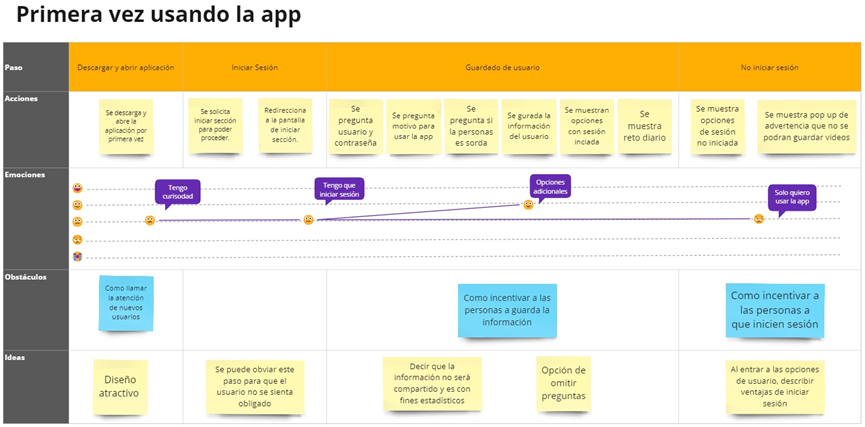
\includegraphics[width=1.1\linewidth]{figuras/mapa_exp1.png}
        \caption{Primera vez usando la aplicación}
        \label{fig:enter-label}
    \end{figure}

    
    \item Grabación de videos, para identificar cómo debe actuar la aplicación para que la funcionalidad sea sencilla.

    \begin{figure} [H]
        \centering
        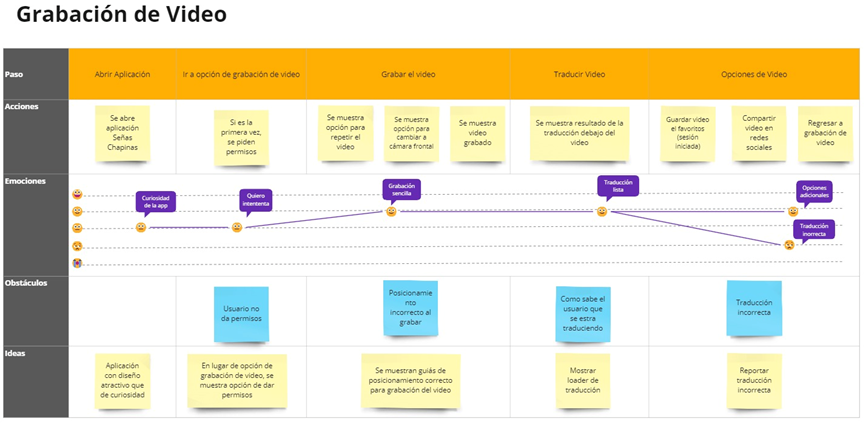
\includegraphics[width=1\linewidth]{figuras/mapa_exp2.png}
        \caption{Grabación de video}
        \label{fig:enter-label}
    \end{figure}
    
    \item Guardado de video, para analizar cómo debe realizarse el proceso.

    \begin{figure} [H]
        \centering
        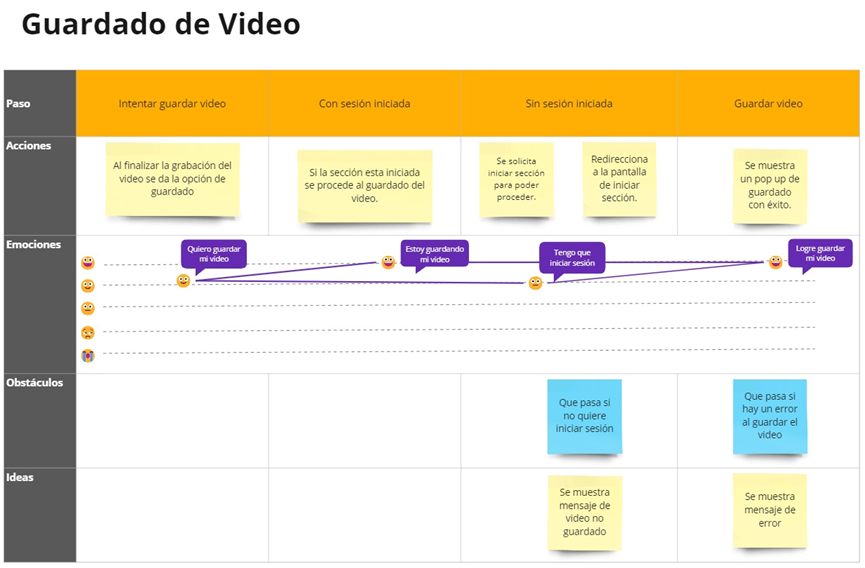
\includegraphics[width=0.9\linewidth]{figuras/mapa_exp3.png}
        \caption{Guardando Video}
        \label{fig:enter-label}
    \end{figure}
        
    \item Reporte de traducción errónea, para facilitar una manera en que los usuarios puedan ayudar a mejorar la aplicación.

    \begin{figure} [H]
        \centering
        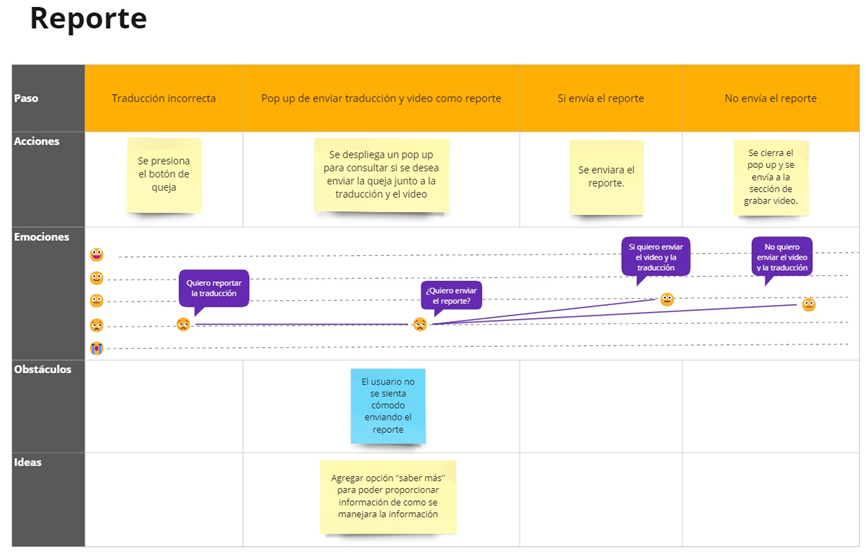
\includegraphics[width=0.95\linewidth]{figuras/mapa_exp4.png}
        \caption{Reporte}
        \label{fig:enter-label}
    \end{figure}
    
    
    \item Diccionario de palabras, para entender de qué manera los usuarios usarían esta herramienta.

    \begin{figure} [H]
        \centering
        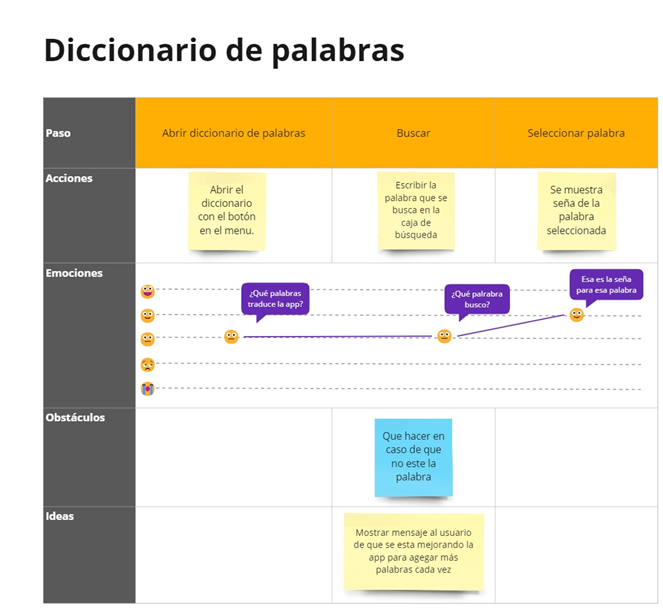
\includegraphics[width=0.7\linewidth]{figuras/mapa_exp5.png}
        \caption{Diccionario de palabras}
        \label{fig:enter-label}
    \end{figure}
    
    \item Reto diario, para identificar puntos de dolor en esta actividad.

    \begin{figure} [H]
        \centering
        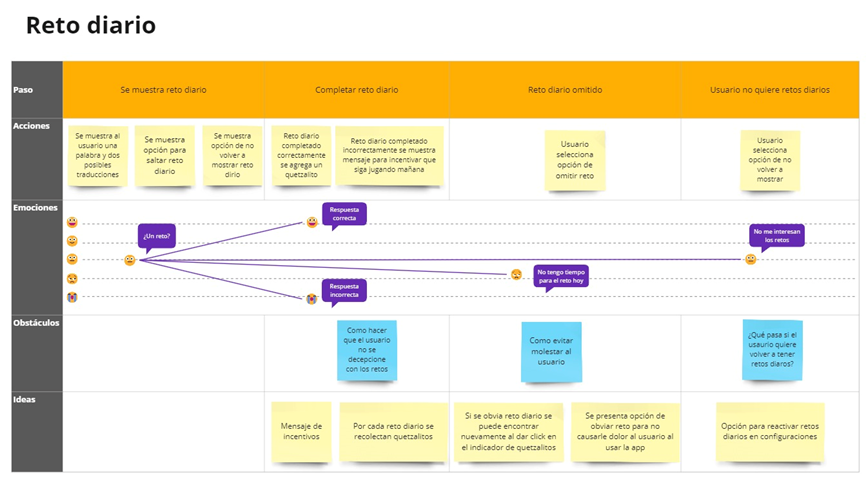
\includegraphics[width=1\linewidth]{figuras/mapa_exp6.png}
        \caption{Reto diario}
        \label{fig:enter-label}
    \end{figure}
\end{itemize}















% -----------------------------------------------------------------------------------------

\subsection{Mapa de Sitio}

Los mapas de sitio proporcionados visualizan la estructura y navegación de la aplicación ``Señas Chapinas'', facilitando un entendimiento claro de las funcionalidades disponibles para los usuarios en diferentes estados.

\begin{itemize}
    \item \textbf{Pantalla para Grabar Video}: Permite a los usuarios grabar para ser traducido a LENSEGUA. 
    \begin{itemize}
        \item \textbf{Compartir video y traducción}: Luego de traducir el video, se puede compartir el video y su traducción.
        \item \textbf{Reportar traducción incorrecta}: Si la traducción es incorrecta, los usuarios pueden reportar errores.
        \item \textbf{Guardar video}: Guardar traducciones realizadas para consultarlas nuevamente.
    \end{itemize}
    \item \textbf{Diccionario de palabras}: Pemite a los usuarios buscar vocabulario disponible para traducción. 
    
    \item \textbf{Perfil}: Acceso a configuraciones de la cuenta.
    \begin{itemize}
        \item \textbf{Información del usuario}: Muestra los detalles del usuario registrado.
        \item \textbf{Racha de retos diarios}: Muestra el progreso del usuario en retos diarios de aprendizaje.
        \item \textbf{Videos Guardados}: Acceso a videos que el usuario ha decidido guardar.
        \begin{itemize}
            \item Al seleccionar un video guardado se acceden a las mismas opciones de video traducido (compartir, reportar o grabar video).
        \end{itemize}
        \item \textbf{Configuración / Sobre la app / Ayuda}: Opciones para mejorar la experiencia del usuario en la aplicación.
        \item \textbf{Cerrar Sesión}: Permite al usuario salir de su cuenta.
    \end{itemize}
\end{itemize}

\begin{figure} [H]
    \centering
    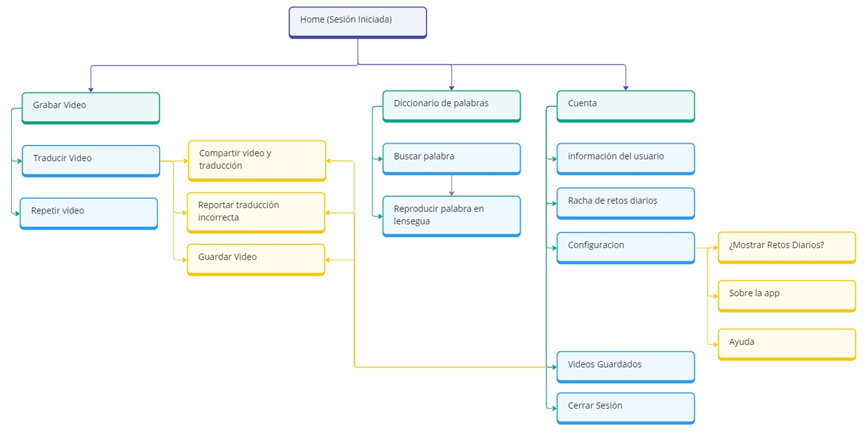
\includegraphics[width=1\linewidth]{figuras/mapa_sitio.png}
    \caption{Mapa de Sitio}
    \label{fig:enter-label}
\end{figure}

% -----------------------------------------------------------------------------------------

\subsection{Flujo de Usuarios}

En el diseño de UX, un flujo de usuarios es una representación visual de los pasos que un usuario sigue dentro de una aplicación para alcanzar un objetivo específico. Esto incluye todas las acciones, decisiones y procesos desde el punto de entrada hasta la salida \cite{Adobe2022}.

Para crear un flujo de usuarios efectivo, es crucial seguir algunos pasos detallados:

\begin{enumerate}
    \item \textbf{Comprender el viaje del cliente}: Con la información recopilada en las Personas, los Mapas de empatía y los Mapas de la experiencia del cliente, se identificaron las necesidades, motivaciones y comportamientos de los usuarios \cite{Adobe2022}.
    
    \item \textbf{Identificar y alinear los objetivos}: Cada sección de la aplicación debe tener un objetivo claro que puede diferir de los objetivos del usuario. Por lo tanto, es esencial identificar lo que los usuarios buscan lograr y alinear los objetivos de la aplicación con los de ellos para asegurar que el flujo de usuario los guíe efectivamente hacia acciones deseadas \cite{Adobe2022}.
    
    \item \textbf{Decidir la información que necesitan los usuarios}: Basado en las Personas y los Mapas del viaje del cliente, se definen los pasos necesarios que los usuarios deben seguir dentro del flujo, abordando sus puntos de dolor y proporcionando la información que buscan en cada etapa \cite{Adobe2022}.
    
    \item \textbf{Visualizar el flujo}: Finalmente, se visualiza y mapea el esquema utilizando formas para comunicar los diferentes caminos y decisiones en un flujo de usuarios \cite{Adobe2022}.
    \begin{itemize}
        \item Los óvalos representan el inicio y el final de un flujo de usuarios.
        \item Los rectángulos simbolizan un paso del proceso, una página de la aplicación.
        \item Las flechas conectan las formas y muestran la dirección del camino del usuario.
        \item Los diamantes representan decisiones que los usuarios toman en cada paso.
        \item Los paralelogramos indican dónde el usuario debe ingresar algo.
        \item El rectángulo redondeado simboliza mensajes al usuario o notificaciones dentro de la aplicación.
    \end{itemize}
    
    \item \textbf{Obtener retroalimentación}: Para mejorar la experiencia en la aplicación, se comparte con usuarios finales para identificar posibles fricciones en el flujo y encontrar formas de agilizar y mejorar las funcionalidades \cite{Adobe2022}.
\end{enumerate}

El primer Flujo de Usuario realizado es para Marta. Marta es sorda profunda y trabaja como cajera por lo que desea ofrecer sus productos de caja para obtener comisiones. Para ello graba un video y reproduce el audio de la traducción. 

\begin{figure} [H]
    \centering
    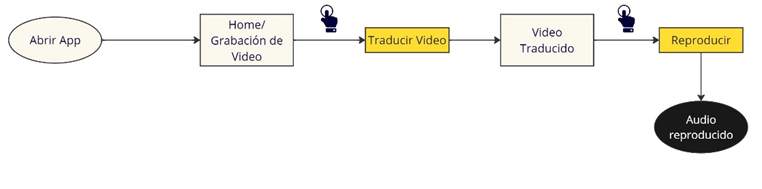
\includegraphics[width=1\linewidth]{figuras/flujo_usuario1.png}
    \caption{Grabar video}
    \label{fig:enter-label}
\end{figure}

Posteriormente se da cuenta que puede guardar el video para usarlo múltiples veces.

\begin{figure}  [H]
    \centering
    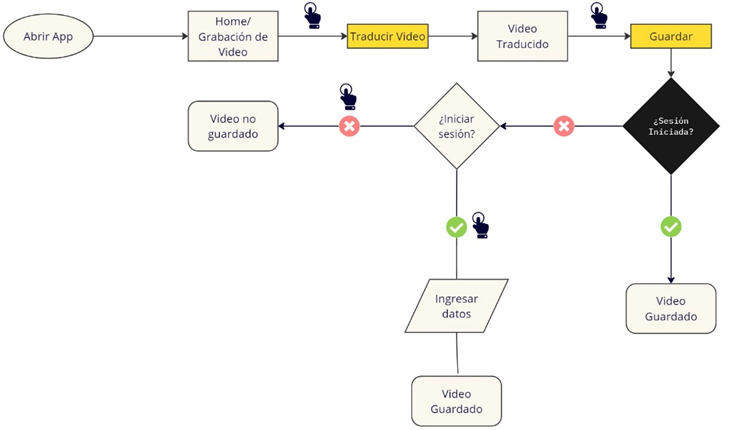
\includegraphics[width=1\linewidth]{figuras/flujo_usuario2.png}
    \caption{Guardar Video}
    \label{fig:enter-label}
\end{figure}

\begin{figure} [H]
    \centering
    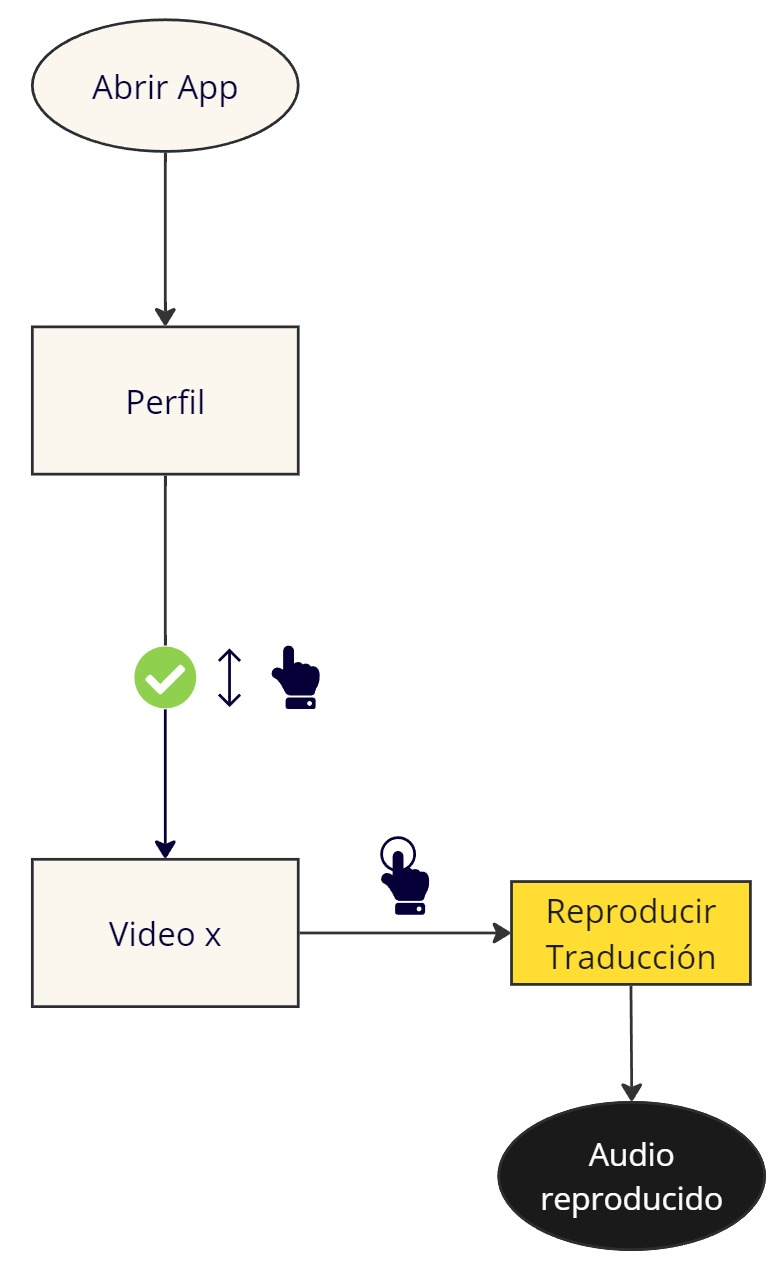
\includegraphics[width=0.3\linewidth]{figuras/flujo_usuario3.jpg}
    \caption{Abrir Video Guardado}
    \label{fig:enter-label}
\end{figure}


Por otra parte, Ricardo tiene sesiones constantemente con sus clientes, por lo que graba y guarda videos constantemente. Adicionalmente, le gusta repetir sus videos para que queden a su gusto. 

\begin{figure} [H]
    \centering
    \includegraphics[width=0.7\linewidth]{figuras/flujo_usuario4.png}
    \caption{Repertir grabación de video}
    \label{fig:enter-label}
\end{figure}


Laura a su vez, al ser madre de un hijo sordo está aprendiendo LENSEGUA. Por eso le parece importante completar los retos diarios. 


\begin{figure} [H]
    \centering
    \includegraphics[width=0.75\linewidth]{figuras/flujo_usuario6.png}
    \caption{Completar reto}
    \label{fig:enter-label}
\end{figure}


Jorge por su parte, al estar aprendiendo LENSEGUA considera muy importante tener traducciones precisas. Por ello al obtener un resultado incorrecto en su traducción, rápidamente reporta el problema.

\begin{figure} [H]
    \centering
    \includegraphics[width=1\linewidth]{figuras/flujo_usuario7.png}
    \caption{Reportar traducción}
    \label{fig:enter-label}
\end{figure}


Sofía es voluntaria por lo que al tener contacto con la comunidad sorda, despertó su interés por aprender LENSEGUA. Por eso accede al diccionario para mejorar su vocabulario. 


\begin{figure} [H]
    \centering
    \includegraphics[width=1\linewidth]{figuras/flujo_usuario8.png}
    \caption{Diccionario}
    \label{fig:enter-label}
\end{figure}


% -----------------------------------------------------------------------------------------

\subsection{Estructura Alámbrica}

Un \textit{Wireframe} o Estructura Alámbrica, es un esquema visual que representa la estructura básica de una aplicación, mostrando el diseño y la disposición de los elementos clave sin entrar en detalles sobre el estilo gráfico o contenido final. Los \textit{Wireframes} utilizan formas simples como rectángulos, líneas y texto básico para indicar elementos como encabezados, párrafos, imágenes y botones \cite{Rees2024}.

\newpage
\begin{itemize}
    \item Baja Fidelidad

        \begin{figure} [H]
            \centering
            \includegraphics[width=0.8\linewidth]{figuras/wireframe_baja.png}
            \caption{Wireframe bajo nivel}
            \label{fig:enter-label}
        \end{figure}
    
    \item Media Fidelidad

        \begin{figure} [H]
            \centering
            \includegraphics[width=0.9\linewidth]{figuras/wireframe_media.png}
            \caption{Wireframe nivel medio}
            \label{fig:enter-label}
        \end{figure}

    \newpage
    \item Alta Fidelidad

        \begin{figure}[H]
            \centering
            \includegraphics[width=1\linewidth]{figuras/fireframe_alta1.png}
            \caption{Wireframe alto nivel}
            \label{fig:enter-label}
        \end{figure}
    
\end{itemize}

Al llegar a este punto del desarrollo de la interfaz y experiencia de usuario se hace\textbf{ una primera validación con usuarios finales}. Se tuvo una reunión con varias personas de En-Señas pertenecientes tanto a la comunidad sorda como a la comunidad oyente. Tomando en cuenta los comentarios y sugerencias de esta validación, se hicieron algunas mejoras.

\begin{itemize}
    \item 
    Se ha añadido una nueva pantalla denominada ``Traducción'' cuyo propósito es permitir que las personas escriban frases en gramática LENSEGUA, que luego son traducidas a gramática española. Esta funcionalidad fue desarrollada en respuesta a los comentarios sobre cómo las personas sordas utilizan herramientas como \textit{ChatGPT} para mejorar su gramática escrita. Es importante destacar que, según los entrevistados, el nivel de comprensión lectora de una persona sorda promedio equivale aproximadamente al de un niño en tercer grado de primaria. Por lo tanto, esta herramienta no solo busca mejorar las habilidades de escritura de las personas sordas. 
    
    \item
    En la pantalla del usuario, se han añadido ahora opciones para marcar como favoritos no solo vídeos sino también traducciones.
    
    \item 
    En el diccionario, se ha implementado que las tarjetas se vuelvan interactivas, funcionando como \textit{flashcards}. Cada tarjeta muestra, por un lado, la palabra acompañada de una imagen, y por el otro, la seña correspondiente. La incorporación de imágenes fue una recomendación de intérpretes, quienes destacaron que las personas sordas tienden a ser muy visuales y que estas representaciones facilitarían significativamente su comprensión de las palabras.
    
\end{itemize}

Teniendo en cuenta estos comentarios y otras sugerencias menores, se realizaron diversas mejoras que culminaron en la creación de un nuevo \textit{Wireframe} de alto nivel.

\begin{figure} [H]
    \centering
    \includegraphics[width=1\linewidth]{figuras/wireframe_alto2.png}
    \caption{Wireframe alto nivel luego de retroalimentación}
    \label{fig:enter-label}
\end{figure}

Se consolida entonces la siguiente estructura para la aplicación:

\begin{enumerate}
    \item \textbf{Pantalla 1: Home}
    \begin{itemize}
        \item \textbf{Función Principal:} Pantalla de inicio.
        \item \textbf{Elementos:}
        \begin{itemize}
            \item Botón principal para grabar video.
            \item Botones adicionales para funcionalidades como cambiar cámara.
            \item Barra de navegación en la parte inferior con cuatro íconos para acceder a las cuatro secciones de la aplicación.
        \end{itemize}
    \end{itemize}

    \item \textbf{Pantalla 2: Traducción de video}
    \begin{itemize}
        \item \textbf{Función Principal:} Mostrar el video grabado junto con su traducción.
        \item \textbf{Elementos:}
        \begin{itemize}
            \item Área de reproducción del video.
            \item Traducción del video en la parte inferior.
            \item Botones para agregar a favoritos, compartir, repetir el video, reportar errores en la traducción y cerrar traducción.
        \end{itemize}
    \end{itemize}

    \item \textbf{Pantalla 3: Traducción de LENSEGUA a español}
    \begin{itemize}
        \item \textbf{Función Principal:} Traducir de gramática de LENSEGUA a gramática española.
        \item \textbf{Elementos:}
        \begin{itemize}
            \item Sección de LENSEGUA para escribir o pegar texto.
            \item Sección de traducción al español para copiar, reproducir o guardar la traducción.
            \item Botón para traducir/nueva traducción.
        \end{itemize}
    \end{itemize}

    \item \textbf{Pantalla 4: Perfil de usuario}
    \begin{itemize}
        \item \textbf{Función Principal:} Mostrar la información del perfil del usuario.
        \item \textbf{Elementos:}
        \begin{itemize}
            \item Ícono de perfil y nombre del usuario.
            \item Contador de días de racha de desafíos completados.
            \item Lista de videos favoritos con sus respectivas traducciones.
            \item Lista de traducciones de LENSEGUA a Español favoritas. 
        \end{itemize}
    \end{itemize}

    \item \textbf{Pantalla 5: Configuración}
    \begin{itemize}
        \item \textbf{Función Principal:} Acceder a las configuraciones de la cuenta.
        \item \textbf{Elementos:}
        \begin{itemize}
            \item Opción par obtener información sobre la aplicación. 
            \item Opción para cerrar sesión y eliminar la cuenta.
            \item Opción para desactivar los retos diarios.
        \end{itemize}
    \end{itemize}

    \item \textbf{Pantalla 6: Diccionario de palabras}
    \begin{itemize}
        \item \textbf{Función Principal:} Mostrar palabras disponibles para traducción.
        \item \textbf{Elementos:}
        \begin{itemize}
            \item Lista de palabras con sus traducciones en LENSEGUA.
            \begin{itemize}
                \item Ordenadas alfabéticamente.
                \item Botón de agregar a favoritos.
            \end{itemize}
            \item Sistema de búsqueda por palabra.
            \item Búsqueda por categorías.
        \end{itemize}
    \end{itemize}

    \item \textbf{Pantalla 7: Desafíos diarios}
    \begin{itemize}
        \item \textbf{Función Principal:} Presentar desafíos diarios de traducción.
        \item \textbf{Elementos:}
        \begin{itemize}
            \item Palabra en español
            \item 4 imágenes de posibles traducciones en LENSEGUA
            \item Opciones para omitir y cerrar el desafío.
        \end{itemize}
    \end{itemize}
\end{enumerate}


% -----------------------------------------------------------------------------------------

\subsection{Logo}

El logo de la aplicación ``Señas Chapinas'' busca simbolizar la comunidad sorda y la cultura guatemalteca. Se escogió un quetzal, el ave nacional de Guatemala, para representar el país, y manos para representar a la comunidad sorda. La evolución del logo refleja una serie de mejoras y refinamientos para lograr un diseño que comunique efectivamente estos valores.

El primer logo integraba ambos componentes: el quetzal y las manos. Las alas y la cola del quetzal se diseñaron para parecerse a manos en señas, representando así tanto la identidad cultural guatemalteca como la lengua de señas. Este diseño inicial se envió a un diseñador gráfico para recibir orientación de como mejorar su forma y funcionalidad.

\begin{figure} [H]
    \centering
    \includegraphics[width=0.75\linewidth]{figuras/primerLogo.png}
    \caption{Primer Logo}
    \label{fig:enter-label}
\end{figure}

El segundo diseño mantuvo la misma idea pero fue vectorizado, simplificado y mejorado en términos de legibilidad y estilo. La vectorización permitió un diseño más limpio y adaptable a diferentes tamaños y medios.

\begin{figure} [H]
    \centering
    \includegraphics[width=0.4\linewidth]{figuras/logo2.png}
    \caption{Logo vectorizado}
    \label{fig:enter-label}
\end{figure}


Para el tercer diseño, se solicitó la colaboración de una diseñadora gráfica con el fin de modernizar el logo. Como resultado, se decidió utilizar solo una mano en lugar de dos, simplificando y actualizando el concepto visual.

\begin{figure} [H]
    \centering
    \includegraphics[width=0.4\linewidth]{figuras/logo3.png}
    \caption{Logo modernizado}
    \label{fig:enter-label}
\end{figure}

En colaboración con la diseñadora gráfica se seleccionaron los colores del logo, incorporando tonos verde, rojo y amarillo que evocan las características distintivas del quetzal y reflejan la identidad cultural guatemalteca. Estos colores no solo realzan visualmente el logo, sino que también fortalecen su vínculo con el patrimonio nacional.

\begin{figure} [H]
    \centering
    \includegraphics[width=0.4\linewidth]{figuras/logo4.png}
    \caption{Logo con colores}
    \label{fig:enter-label}
\end{figure}

Finalmente, se logró el diseño definitivo: un logo colorido y moderno que refleja la cultura de Guatemala a través del símbolo del quetzal y representa a la comunidad sorda con la imagen de una mano utilizando LENSEGUA. Este logo combina simplicidad, modernidad y simbolismo cultural, proporcionando una representación atractiva y efectiva para la aplicación. 


\begin{figure} [H]
    \centering
    \includegraphics[width=0.4\linewidth]{figuras/logo_final.png}
    \caption{Logo Señas Chapinas}
    \label{fig:enter-label}
\end{figure}



% -----------------------------------------------------------------------------------------

\subsection{Paleta de Colores}


Los colores seleccionados para el logo son los siguientes:


\begin{itemize}
    
    \item \textbf{Verde Quetzal (\#00973A):} Este color representa al quetzal y simboliza vida y esperanza. 
       
    \item \textbf{Rojo (\#E20613):}  Su uso en la aplicación es para indicar errores o acciones importantes, facilitando al usuario identificar problemas o acciones críticas dentro de la aplicación.

    \item \textbf{Verde Lima (\#93C01F):} Se utiliza para dar mas detalle al quetzal y para el título de la aplicación porque tiene mayor contraste con el azul del fondo. 
    
    \item \textbf{Amarillo (\#FFDD00):}) Usado para destacar el pico del quetzal en el logo, este amarillo no solo contrasta eficazmente con los verdes, sino que también simboliza felicidad y acción. 

    \item \textbf{Azul (\#29235C):}) Aunque el azul tradicional de la bandera de Guatemala es más claro, se ha seleccionado un tono azul oscuro para conferir profundidad y seriedad al logo
    
\end{itemize}

\begin{figure} [H]
    \centering
    \includegraphics[width=0.25\linewidth]{figuras/paleta_colores_logo.png}
    \caption{Paleta de colores logo}
    \label{fig:enter-label}
\end{figure}


Con base a estos colores, también se seleccionaron los colores para la aplicación, buscando no solo impacto visual, sino también  fortalecer la conexión con la identidad cultural guatemalteca.

\begin{itemize}
    \item \textbf{Azul (\#29235C):} Se utiliza principalmente como color para texto de la aplicación. Ofrece legibilidad y una sensación de seguridad y confianza.  
    
    \item \textbf{Verde Quetzal (\#00973A):} Se usa para botones y títulos, aportando vitalidad y energía a la interfaz. 
       
    \item \textbf{Rojo (\#E20613):} Se utuliza para indicar errores o acciones importantes, facilitando al usuario identificar problemas o acciones críticas dentro de la aplicación.

    \item \textbf{Blanco Crema (\#F5F5F5):} Se utiliza como fondo para la aplicación. En lugar del blanco puro, este tono crema proporciona una suavidad que puede ser menos agresiva a la vista. 
    
    \item \textbf{Gris Carbón (\#323232):} Se utiliza principalmente como fondo de pantallas de temporales. Es un color neutro elegido específicamente para minimizar las distracciones y evitar que los usuarios permanezcan en estas pantallas transitorias por más tiempo del necesario, a diferencia del uso de los colores azul y blanco en otras secciones de la aplicación, que buscan captar y mantener la atención del usuario.

\begin{figure} [H]
    \centering
    \includegraphics[width=0.6\linewidth]{figuras/paleta_colores.png}
    \caption{Paleta de colores aplicación}
    \label{fig:enter-label}
\end{figure}

    
    
\end{itemize}

Con base a la paleta de colores del logo, se obtienen colores pastel utilizados para el quetzal de perfil del usuario y las opciones del reto diario:

\begin{itemize}

    \item Aqua Pastel (\#37B7C3)
    \item Azul Pastel (\#83B4FF)
    \item Verde Pastel (\#8DC249)
    \item Amarillo Pastel (\#FCB424)

\end{itemize}

\begin{figure} [H]
    \centering
    \includegraphics[width=0.5\linewidth]{figuras/paleta_colores_quetzal.png}
    \caption{Paleta Colores Perfil}
    \label{fig:enter-label}
\end{figure}

Asimismo también se comprueban contrastes de los colores seleccionados:

\begin{itemize}

    \item \textbf{Azul y Blanco:} Los colores azul y blanco seleccionados presentan un contraste óptimo, lo cual justifica su uso como fondo y texto principales en la aplicación. 

    \begin{figure} [H]
        \centering
        \includegraphics[width=0.6\linewidth]{figuras/contraste_azul_blanco.png}
        \caption{Contraste blanco y azul}
        \label{fig:enter-label}
    \end{figure}


    \begin{figure} [H]
        \centering
        \includegraphics[width=0.6\linewidth]{figuras/contraste_blanco_azul.png}
        \caption{Contraste azul y blanco}
        \label{fig:enter-label}
    \end{figure}

  
    \item \textbf{Contraste gris y blanco:} Los colores gris y blanco seleccionados ofrecen un contraste adecuado, lo cual los hace idóneos para su uso en las pantallas temporales. 

    \begin{figure} [H]
        \centering
        \includegraphics[width=0.6\linewidth]{figuras/contraste_gris_blanco.png}
        \caption{Contraste gris y blanco}
        \label{fig:enter-label}
    \end{figure}
    
    
    \item \textbf{Constraste blanco y rojo:}  Aunque el contraste entre blanco y rojo no es tan alto como en otros casos, aún cumple con los requisitos mínimos recomendados. Este se utiliza exclusivamente en situaciones necesarias para alertar al usuario sobre una acción crítica.

    \begin{figure} [H]
        \centering
        \includegraphics[width=0.6\linewidth]{figuras/contraste_blanco_rojo.png}
        \caption{Contraste blanco y rojo}
        \label{fig:enter-label}
    \end{figure}
    
    \item \textbf{Contraste verde quetzal y azul:} El contraste entre el verde quetzal es ligeramente inferior al nivel recomendado. Por esta razón, se empleará únicamente para elementos destacados como títulos grandes, botones y el logo, donde la legibilidad sigue siendo efectiva a pesar del menor contraste. 
   
    \begin{figure} [H]
        \centering
        \includegraphics[width=0.6\linewidth]{figuras/contraste_azul_verde.png}
        \caption{Constraste verde quetzal y azul}
        \label{fig:enter-label}
    \end{figure}

    \item \textbf{Contraste verde claro y azul:} El contraste entre el verde claro y el azul cumple con las normas recomendadas, razón por la cual se ha seleccionado para el título de la aplicación
    
    \begin{figure} [H]
        \centering
        \includegraphics[width=0.6\linewidth]{figuras/contraste_verde_claro_azul.png}
        \caption{Constraste verde claro y azul}
        \label{fig:enter-label}
    \end{figure}
        

\end{itemize}


% -----------------------------------------------------------------------------------------

\subsection{Tipografía}

La tipografía recomendada por la diseñadora gráfica para el logo de ``Señas Chapinas'' fue Adonide Bold. Esta elección se justifica por su claridad y modernidad, cualidades que reflejan la simplicidad y accesibilidad que la aplicación busca transmitir. Adonide Bold es una fuente sans-serif que ofrece un aspecto limpio y profesional, ideal para destacar en logotipos y cabeceras por su legibilidad y presencia  \cite{AdonideFont}.

Con base a esa tipografía y al contexto de la aplicación, se decide utilizar Nunito para el contenido de la misma. Nunito, también una sans-serif disponible gratuitamente en \textit{Google Fonts}, es conocida por sus curvas suaves y su legibilidad en interfaces digitales, lo que la hace ideal para textos largos y elementos de interfaz de usuario en aplicaciones móviles. Su diseño amigable y accesible complementa perfectamente la estética introducida por Adonide Bold en el logo, asegurando coherencia visual y facilitando la experiencia del usuario al navegar por la aplicación. Esta elección refuerza el objetivo de la aplicación de ser accesible y fácil de usar, elementos cruciales para una herramienta destinada a mejorar la comunicación en la comunidad sorda \cite{Design2024}.

\begin{figure} [H]
    \centering
    \includegraphics[width=0.75\linewidth]{figuras/tipografia.png}
    \caption{Tipografía Nunito}
    \label{fig:enter-label}
\end{figure}

% -----------------------------------------------------------------------------------------

\subsection{Prototipos}

Al concluir la fase de diseño UX/UI, se han definido claramente las necesidades de los usuarios, así como los flujos principales de la aplicación. Durante este proceso, también se seleccionaron cuidadosamente los colores y la tipografía que mejor se adaptan a la experiencia del usuario, garantizando así coherencia visual y funcionalidad. Con estos elementos bien establecidos, el siguiente paso ha sido la creación de prototipos detallados en Figma. Este enfoque permite simular la interacción del usuario con la aplicación.

\subsubsection{Prototipo de Bajo Nivel}
Este primer prototipo tiene como objetivo demostrar la funcionalidad general de la aplicación sin enfocarse en el diseño de colores, presentando una estructura básica. Para ver el diseño con más detalles consultar: \href{https://www.figma.com/design/d7NOw36r1mUY7qDBIveJ2K/Se%C3%B1as-Chapinas?node-id=45-820&node-type=SECTION&t=luJsnsyUNaEJGP24-0}{Figma}.

\begin{itemize}
    \item \textbf{Barra de Navegación:} Contiene las opciones de ``Video'', ``Traductor'', ``Diccionario'' y ``Perfil''. La opción seleccionada se destaca visualmente sobre las demás.
    
    \item \textbf{Pantalla de Inicio:} Ofrece la función principal de grabar video. Al presionar el botón correspondiente, el video comienza a grabarse.
    
    \item \textbf{Pantalla de Video:} Muestra el video grabado junto con opciones para reportar errores, agregar a favoritos, compartir, repetir, utilizar el altavoz y cerrar. Las traducciones en español y LENSEGUA se muestran en la parte inferior.
    
    \item \textbf{Reporte de Traducción:} Un modal que permite al usuario reportar errores en la traducción. Antes de continuar, se solicita revisar el diccionario. Luego, el usuario puede proceder con el reporte.
    
    \item \textbf{Traductor:} Al ingresar, se presenta un área para escribir o pegar texto en LENSEGUA. El botón de traducción está deshabilitado hasta que el usuario ingrese el texto. Una vez ingresado, el botón se habilita, y al presionarlo, se muestra la traducción al español junto con las opciones de copiar, escuchar con el altavoz, agregar a favoritos o realizar una nueva traducción.
    
    \item \textbf{Diccionario:} Muestra tarjetas redondeadas que representan las palabras disponibles. Las tarjetas se pueden agregar a favoritos. En la parte superior, se incluye una barra de búsqueda y la opción de seleccionar por categorías. Además, cuenta con una barra de desplazamiento para navegar entre las tarjetas ordenadas alfabéticamente.
    
    \item \textbf{Perfil del Usuario:} Muestra una imagen de perfil, el nombre del usuario y un contador de días consecutivos de desafíos completados. También incluye un ícono de configuración en la parte superior para acceder a ajustes. La pantalla presenta una barra de pestañas que permite alternar entre los videos favoritos y las traducciones favoritas.
    
    \item \textbf{Configuraciones:} Ofrece opciones para cambiar la contraseña, cerrar sesión, eliminar la cuenta y acceder a información sobre la aplicación. También permite activar o desactivar los retos diarios, ver un tutorial y consultar la versión actual de la app.
    
    \item \textbf{Retos Diarios:} Presenta cuatro imágenes como opciones de respuesta para una palabra en LENSEGUA. El usuario puede elegir una respuesta, o bien, cerrar u omitir el reto. Las opciones se presentan en un diálogo interactivo.
\end{itemize}

Cabe destacar que el diseño del primer prototipo se caracteriza por su simplicidad e intuición, con un uso mínimo de texto para facilitar la navegación. Basado en las recomendaciones de los usuarios finales, se utilizaron como referencia aplicaciones que ellos consideran fáciles de usar, adaptando y personalizando el diseño a la identidad y necesidades únicas de la aplicación 'Señas Chapinas'. Un ejemplo de ello es la disposición de las opciones en la pantalla de video, que recuerda a la aplicación \textit{TikTok}.

\begin{figure} [H]
    \centering
    \includegraphics[width=1\linewidth]{figuras/Prototipo1.png}
    \caption{Primer Prototipo}
    \label{fig:primer_prototipo}
\end{figure}

\subsubsection{Prototipo de Nivel Medio}

Tras presentar el primer prototipo a los usuarios finales, se realizaron algunos ajustes visuales menores, como la modificación del tamaño del texto y de los íconos. Después de implementar estos cambios y obtener la aprobación de los usuarios, se desarrolló el segundo prototipo. Este incluyó pantallas para el inicio de sesión y la creación de cuenta, una pantalla de inicio, una pantalla para cambio de contraseña, y una pantalla con descripción de la aplicación. Además, se empezó a integrar color y mejorar la navegación. Para analizar con más detalle revisar: \href{https://www.figma.com/design/d7NOw36r1mUY7qDBIveJ2K/Se%C3%B1as-Chapinas?node-id=275-15737&node-type=CANVAS&t=ua1wEji5yxVRI6ES-0}{Figma} 


\begin{figure} [H]
    \centering
    \includegraphics[width=1\linewidth]{figuras/segundo_prototipo.png}
    \caption{Segundo Prototipo}
    \label{fig:segundo_prototipo}
\end{figure}

\subsubsection{Prototipo de Alto Nivel}

El tercer prototipo muestra ya el diseño completo de la aplicación, para ver mas a detalle revisar \href{https://www.figma.com/design/d7NOw36r1mUY7qDBIveJ2K/Se%C3%B1as-Chapinas?node-id=322-1684&node-type=CANVAS&t=ua1wEji5yxVRI6ES-0}{Figma}:

\begin{itemize}
    \item \textbf{Pantalla de \textit{Splash}:} Fondo azul con el logo y nombre de la aplicación.
  
    \item \textbf{Pantalla de Inicio:} En la parte superior se muestra el logo y el nombre, seguido por el eslogan en español y LENSEGUA. También se incluyen los botones ``Empezar Ahora'', que lleva a la creación de cuenta, y ``Ya tengo una cuenta'', para iniciar sesión.
  
    \item \textbf{Creación de Cuenta:} El logo y el nombre se presentan en la parte superior azul, mientras que en la parte inferior blanca se muestran los campos para ingresar el correo, la contraseña y la confirmación de contraseña. Se incluyen dos botones:``Empezar Ahora'', que continúa con el flujo, y ``Ya tengo una cuenta'', para redirigir al login.
  
    \item \textbf{Grabación de Video:} Muestra la simulación de la toma de video, con un botón de grabación al centro y una barra de navegación inferior que incluye las opciones de video, traducción, diccionario y perfil.

    \item \textbf{Video:} Presenta una simulación del video grabado con opciones en la parte superior para reportar, agregar a favoritos, compartir y repetir el video. En la parte inferior se muestra la traducción en LENSEGUA y español. Se usa iconografía estándar en lugar de texto para facilitar la navegación a las personas sordas.

    \item \textbf{Reportar:} A diferencia del primer prototipo, ya no se utiliza un modal, sino un \textit{bottom sheet}, de acuerdo con las recomendaciones de un experto en diseño, ya que es más dinámico, moderno y menos intrusivo. El título se presenta en rojo para resaltar que es una acción crítica. Se le pide al usuario que revise si la palabra existe en el diccionario antes de reportarla, y se muestran botones con el ícono del diccionario utilizado en la barra de navegación, cumpliendo con la solicitud de las personas sordas de utilizar iconografía y no solo texto. El botón de reportar también es rojo, ya que se trata de una acción crítica. Al finalizar el flujo de reporte, se muestra un mensaje confirmando que el reporte ha sido generado.

    \item \textbf{Traductor:} A diferencia del primer prototipo, se introduce un fondo azul en el área de ingreso de texto en LENSEGUA y un fondo blanco para el texto traducido en español. Se ha añadido un límite máximo de palabras para ingresar, a solicitud del equipo de inteligencia artificial. Al igual que en el primer prototipo, el botón de traducir es verde, para resaltar la acción. Este permanece deshabilitado hasta que el usuario ingrese texto en LENSEGUA. Al hacer clic en el botón de traducir, se bloquea la edición del texto en LENSEGUA, y el botón cambia a "Nueva Traducción". Posteriormente, se muestra la traducción en español y las opciones para copiar, usar el altavoz y agregar a favoritos, manteniendo el uso de iconografía en lugar de texto.

    \item \textbf{Diccionario:} El diseño de las tarjetas ha cambiado ligeramente en comparación con el primer prototipo. Ahora se incluye un ícono que indica que la tarjeta se puede voltear, y se ha reducido el redondeado y sombreado de las tarjetas. La barra de búsqueda se mantiene en la parte superior. En las categorías, se ha agregado la sección de favoritos con un ícono de corazón, manteniendo la coherencia de la app, donde los favoritos siempre se representan con un corazón. También se ha incorporado un estado vacío \textit{(empty state)} para cuando no haya resultados en la búsqueda o no se hayan guardado favoritos.

    \item \textbf{Perfil:} A diferencia del primer prototipo, donde el usuario podía seleccionar su propia imagen de perfil, se decidió que la aplicación asignará un color al quetzal del logo, para cada usuario. Se sigue mostrando el nombre del usuario y la racha de desafíos en la parte inferior de la imagen de perfil. Además, el diseño de los favoritos, tanto de videos como de traducciones, ha sido ajustado para añadir más formalidad y dinamismo a la aplicación. También se incluyen flujos para borrar favoritos y pantallas de estado vacío cuando no haya favoritos guardados.

    \item \textbf{Configuración:} El diseño de la sección de configuración ha cambiado respecto al primer prototipo. Ahora incluye subconjuntos de opciones e iconografía para facilitar la navegación del usuario. Además, se ha añadido el flujo de eliminación de cuenta, que se muestra mediante un bottom sheet con un título en rojo, dado que es una acción crítica. El diseño de la sección ``Acerca de la Aplicación'' también ha sido ajustado ligeramente y se han añadido los colaboradores.

    \item \textbf{Reto Diario:} El diseño de la pantalla de retos diarios fue uno de los más desafiantes, ya que no se sabía cómo proporcionar retroalimentación clara cuando el usuario seleccionaba una opción incorrecta, ni cómo manejar las rachas de forma visual. Finalmente, se decidió por una pantalla que en la parte superior muestra la racha actual, un título llamativo, y la palabra objetivo a seleccionar en las tarjetas. Las tarjetas utilizan colores pastel, y en la parte inferior se encuentra la opción de omitir. Cuando la respuesta es correcta, se añade un punto a la racha y aparece una animación de confeti. Si la respuesta es incorrecta, la racha se restablece a cero, el ícono de la racha cambia de color, y se muestra un mensaje para motivar al usuario a intentarlo de nuevo. La tarjeta correcta se muestra en un color más claro que las demás después de que el usuario haya seleccionado una opción. A diferencia del primer prototipo, esta es una pantalla completa y no un modal.

     \item \textbf{Cambio de Contraseña:} Al igual que en el primer prototipo, se muestra el flujo para cambiar la contraseña utilizando el mismo diseño empleado en las pantallas de inicio de sesión y creación de cuenta, manteniendo una coherencia visual en toda la aplicación.

    \item \textbf{Diálogos Adicionales:} Se han integrado diálogos estándar para mostrar mensajes, como alertas de error, y un loader para indicar la ejecución de llamadas a servicios. 
        
\end{itemize}

\begin{figure} [H]
    \centering
    \includegraphics[width=1\linewidth]{figuras/tercer_prototipo.png}
    \caption{Tercer Prototipo}
    \label{fig:enter-label}
\end{figure}


\subsubsection{Cambios Prototipo de Alto Nivel}

Después de presentar el prototipo a expertos en tecnología y usuarios finales, se realizaron varios cambios para mejorar la experiencia del usuario:

\begin{itemize}
    \item \textbf{Pantalla de Creación de Cuenta:} Se eliminó el campo de confirmación de contraseña. En su lugar, se añadió un icono de ojo en el campo de contraseña para mostrar u ocultar la misma, permitiendo que el usuario confirme su contraseña sin necesidad de un campo adicional. Además, se implementaron validaciones de longitud y caracteres necesarios para cumplir con los requisitos de seguridad.
    
    \item \textbf{Pantalla de Inicio de Sesión:} Se agregó un campo para "Olvidé mi contraseña", facilitando a los usuarios la recuperación de su contraseña.
    
    \item \textbf{Pantalla de Inicio:} Se introdujo la opción para que los usuarios elijan si desean activar su cámara al iniciar la aplicación. Si optan por no hacerlo, aparece una pantalla gris temporal que incentiva al usuario a abrir su cámara mediante un botón en la parte inferior. Esta configuración se puede ajustar en las opciones de la aplicación. Además, se añadió una pantalla de solicitud de permisos.
    
    \item \textbf{Pantalla de Grabación de Video:} Se añadió un botón para cambiar la cámara y un acceso directo a videos favoritos. También se incorporó una guía de posicionamiento correcto para el rostro.
    
    \item \textbf{Pantalla de Video Grabado:} El diseño de esta pantalla cambió ligeramente respecto a los prototipos anteriores. Las opciones de video como reportar, altavoz, favoritos y compartir se trasladaron a la parte inferior, junto con el cuadro de traducciones en español y LENSEGUA. Esto se hizo para reflejar que estas opciones se aplican al texto traducido y no al video en sí. Además, el botón de repetir video se eliminó por ser redundante; cerrando el video grabado, es posible grabar uno nuevo.
    
    \item \textbf{Pantalla de Traducción:} Se eliminó la opción de pegar directamente, ya que esta función es accesible manteniendo presionado el campo de entrada. Se añadió un acceso directo a traducciones favoritas.
    
    \item \textbf{Pantalla de Diccionario:} Se sugirió cambiar el color de las tarjetas para añadir más colorido a la pantalla.
    
    \item \textbf{Pantalla de Configuraciones:} Se añadió una opción para activar la cámara al iniciar la aplicación.
    
    \item \textbf{Pantalla de Reto Diario:} El funcionamiento de esta pantalla fue modificado respecto al prototipo anterior. Ahora, cuando el usuario selecciona una opción incorrecta, esta se torna más pálida y vibra. Cuando selecciona la opción correcta, las demás opciones se atenúan, destacando la respuesta correcta. Esto garantiza que el usuario siempre aprenda cuál es la opción correcta y no se frustre al perder su racha, ya que la única forma de perder es no completar el reto diario. Se agregó un botón de cerrar para regresar a la pantalla de inicio.
\end{itemize}

Asimismo, se realizaron ajustes para adaptar la aplicación a diferentes largos de texto. Se efectuaron algunos cambios en el tamaño del texto, el reposicionamiento de iconos, y otros ajustes menores, todo ello con el fin de optimizar la legibilidad y la usabilidad en diversos dispositivos.


\begin{figure} [H]
    \centering
    \includegraphics[width=1\linewidth]{figuras/prototipo4.png}
    \caption{Cuarto Prototipo}
    \label{fig:enter-label}
\end{figure}



% ===========================================================================================

\section{DESARROLLO MÓVIL}

\subsection{Descripción General del Desarrollo Móvil}

La aplicación ``Señas Chapinas'' está desarrollada para dispositivos \textit{Android} utilizando \texttt{Java} para la lógica y el desarrollo principal. Se busca ofrecer una experiencia de usuario intuitiva y accesible, utilizando arquitecturas modernas y prácticas eficientes para garantizar un rendimiento óptimo.

En cuanto al diseño de la interfaz, se optó por el uso de \texttt{XML} en lugar de \texttt{Jetpack Compose}. Este enfoque fue elegido por su madurez, estabilidad y la familiaridad que ofrece a los desarrolladores. Además, \texttt{XML-based UI} permite un mayor control sobre el diseño de las pantallas y una fácil integración con herramientas como \texttt{View Binding} \cite{DeLaGrana2024}.

Para facilitar la vinculación entre las vistas y el código, se utilizó \texttt{View Binding}. Esta herramienta elimina la necesidad de métodos como \texttt{findViewById()}, mejorando la eficiencia y reduciendo errores al acceder a los elementos de la interfaz directamente desde el código \cite{Ozaltun2022}.

La estructura de la aplicación está centrada en un único \texttt{MainActivity}, que gestiona la navegación entre \textit{Home}, \textit{Traducción}, \textit{Diccionario}, y \textit{Perfil} mediante \texttt{NavController} y gráficos de navegación (\texttt{NavGraphs}) independientes para cada sección. Esta decisión permite mantener un código más ordenado y modular, al mismo tiempo que se simplifica la navegación dentro de la aplicación, evitando la complejidad que supondría utilizar varios \texttt{Activities}.

La aplicación incluye un \texttt{Bottom Navigation Menu} para facilitar la navegación entre las diferentes secciones. Este menú se sincroniza con el \texttt{NavController} para permitir transiciones fluidas entre los diferentes \texttt{Fragments} de la aplicación.

% -----------------------------------------------------------------

\subsection{Tecnologías y Librerías}

La aplicación utiliza una variedad de librerías modernas para optimizar su rendimiento y funcionalidad:

\begin{itemize}
    \item \texttt{AndroidX:} Para garantizar compatibilidad y soporte con las versiones más recientes de Android, así como un diseño visual coherente y moderno.
    \item \texttt{View Binding:} Para gestionar de manera eficiente la vinculación de vistas.
    \item \texttt{SharedPreferences:} Utilizado para almacenar configuraciones del usuario, como el estado de inicio de sesión, de manera persistente entre las sesiones de uso de la aplicación.
    \item \texttt{LiveData y ViewModel:} Cada Fragment tiene su propio ViewModel para gestionar de forma eficiente los cambios de estado y lógica de la interfaz de usuario.
    \item \texttt{Navigation Component:} Para gestionar la navegación entre Fragments de manera flexible y organizada.
    \item \texttt{Glide:} Para la carga y manipulación de imágenes de forma eficiente.
    \item \texttt{CameraX:} Para implementar funcionalidades relacionadas con la captura de video.
    \item \texttt{ExoPlayer:} Para la reproducción de videos de alta calidad dentro de la aplicación.
    \item \texttt{Gson:} Para la serialización y deserialización de datos JSON.
    \item \texttt{Lottie:} Para integrar animaciones ligeras y dinámicas en la interfaz de usuario.
\end{itemize}

% -----------------------------------------------------------------

\subsection{Arquitectura del Proyecto}

El proyecto sigue el patrón arquitectónico \textit{Model-View-ViewModel} (MVVM) para organizar el código de manera eficiente y mantener la separación de responsabilidades entre la lógica de negocio, la interfaz de usuario y la manipulación de los datos.

\subsubsection{Organización de la Aplicación}

La aplicación se gestiona con una única \texttt{MainActivity}, que centraliza la navegación y la interacción del usuario. Cada una de las secciones principales de la aplicación (\textit{Home}, \textit{Traducción}, \textit{Diccionario}, y \textit{Perfil}) cuenta con su propio \texttt{NavGraph} para gestionar de forma modular y ordenada los flujos de navegación entre los diferentes \texttt{Fragments}. Este enfoque permite que las diferentes secciones se mantengan independientes, favoreciendo el mantenimiento y escalabilidad del código.

\subsubsection{Gestión de Estados}

Cada \texttt{Fragment} extiende de un \texttt{BaseFragment}, que contiene la lógica compartida entre ellos, como la navegación, la gestión de diálogos personalizados y el manejo de la barra de navegación inferior. Además, cada \texttt{Fragment} cuenta con su propio \texttt{ViewModel}, que hereda de un \texttt{BaseViewModel}. Esto permite gestionar los cambios de estado y lógica específicos de cada pantalla de forma eficiente y organizada, manteniendo los datos y los cambios de estado en el ciclo de vida adecuado, independientemente de los cambios en la interfaz.

\subsubsection{Navegación}

La navegación en la aplicación es gestionada mediante el componente \textit{Navigation Component}, y las transiciones entre los \texttt{Fragments} se gestionan a través de un \texttt{NavController} central, que se sincroniza con el \texttt{Bottom Navigation Menu} para ofrecer una experiencia de usuario fluida. Este enfoque también simplifica el manejo del historial de navegación, permitiendo una interacción más intuitiva para el usuario.

\begin{figure} [H]
    \centering
    \includegraphics[width=0.4\linewidth]{figuras/navegacion_principal.png}
    \caption{Navegación Principal}
    \label{fig:enter-label}
\end{figure}

\begin{figure} [H]
    \centering
    \includegraphics[width=0.4\linewidth]{figuras/navegacion_video.png}
    \caption{Navegación Video}
    \label{fig:enter-label}
\end{figure}

\begin{figure} [H]
    \centering
    \includegraphics[width=0.4\linewidth]{figuras/navegacion_perfil.png}
    \caption{Navegación Perfil}
    \label{fig:enter-label}
\end{figure}

\begin{figure} [H]
    \centering
    \includegraphics[width=0.2\linewidth]{figuras/diccionario.png}
    \caption{Diccionario}
    \label{fig:enter-label}
\end{figure}


\begin{figure} [H]
    \centering
    \includegraphics[width=0.2\linewidth]{figuras/tarduccion.png}
    \caption{Traducción}
    \label{fig:enter-label}
\end{figure}


% ----------------------------------------------

\subsection{Componentes Reutilizables}

En el desarrollo de la aplicación móvil , se ha implementado una serie de componentes reutilizables con el objetivo de mantener un código más modular, flexible y fácil de mantener. A continuación se describen algunos de los componentes más importantes:

\begin{itemize}
    \item \textbf{DebounceClickListener:} Este componente evita múltiples clics en un corto periodo de tiempo sobre un mismo botón, lo cual es útil en situaciones donde los usuarios pueden hacer clic repetidamente. El \texttt{DebounceClickListener} permite que solo se ejecute la acción del clic una vez dentro de un intervalo de tiempo definido, mejorando la experiencia de usuario y previniendo errores.

    \item \textbf{Interfaz para todos los botones:} Para garantizar consistencia y facilitar la extensión de funcionalidades, se implementó una interfaz común para todos los botones de la aplicación. Esta interfaz define métodos para habilitar o deshabilitar los botones, cambiar su estilo y gestionar eventos de clic de manera uniforme.

    \item \textbf{TransparentButton y MainButton:} Son dos variantes de botones reutilizables. El \texttt{\allowdisplaybreaks{Transpa\-rentButton}} se utiliza principalmente para botones secundarios, donde el fondo es transparente pero el borde y el texto son visibles. Por otro lado, el \texttt{MainButton} es para botones primarios con fondo sólido y mayor visibilidad. Ambos botones mantienen un estilo consistente en la aplicación y se pueden personalizar según el contexto.


    \item \textbf{CustomDialogFragment:} Este componente es una implementación personalizada de un \texttt{DialogFragment}, utilizado para mostrar diálogos de manera consistente en toda la aplicación. \texttt{CustomDialogFragment} permite personalizar el contenido, la apariencia y las acciones disponibles para el usuario, como confirmaciones o advertencias.

    \item \textbf{Interfaz para todos los Inputs:} Se creó una interfaz común para los campos de entrada (\textit{inputs}) de la aplicación, lo que asegura un comportamiento coherente en todos los campos de texto. Esto facilita la validación de datos y el manejo de errores, reduciendo la duplicación de código y mejorando la consistencia visual y funcional.

    \item \textbf{InputEmail:} Componente especializado en la validación de correos electrónicos, asegurando que el usuario ingrese una dirección válida. \texttt{InputEmail} detecta errores comunes, como la falta de un símbolo "\texttt{@}" o un dominio incorrecto, e incluye retroalimentación visual para guiar al usuario.

    \item \textbf{InputPassword:} Este componente incluye validaciones centradas en la seguridad, como la longitud mínima de la contraseña, y permite mostrar u ocultar los caracteres ingresados. Esto ayuda al usuario a verificar visualmente su contraseña sin comprometer la seguridad.

    \item \textbf{BottomNavMenu:} Este componente gestiona la navegación entre las principales secciones de la aplicación (\textit{Home}, \textit{Traducción}, \textit{Diccionario}, \textit{Perfil}) mediante una barra de navegación inferior. El \texttt{BottomNavMenu} se integra con el \texttt{NavController}, permitiendo transiciones fluidas entre los diferentes \texttt{Fragments}.

    \item \textbf{CustomProgressBarDialog:} Diálogo personalizado utilizado para mostrar una barra de progreso durante operaciones que pueden tomar tiempo, como la carga de datos. Proporciona una retroalimentación visual clara de las acciones que se están ejecutando en segundo plano.
\end{itemize}

La creación de estos componentes reutilizables asegura que la aplicación mantenga una estructura limpia y eficiente. Además, facilita realizar modificaciones o mejoras sin tener que duplicar código, permitiendo la escalabilidad del proyecto y asegurando que los cambios se propaguen de manera consistente en toda la aplicación.


% ----------------------------------------------

\subsection{Implementación de Seguridad}

\textbf{Autenticación:} El sistema de autenticación de la aplicación se maneja a través de un servicio externo, el cual garantiza la seguridad en el manejo de credenciales y datos sensibles. Las funciones de inicio de sesión y registro están integradas de forma segura mediante API externas.

\textbf{Cifrado:} Los datos del usuario, incluyendo preferencias de configuración y estado de inicio de sesión, se almacenan de forma segura utilizando \textit{SharedPreferences} cifrados. Esto garantiza que la información personal del usuario se mantenga protegida incluso cuando se almacena localmente en el dispositivo.

\textbf{Permisos:} La aplicación solicita únicamente el permiso para acceder a la cámara, utilizado durante la grabación de videos para traducir a LENSEGUA. Este permiso se solicita solo cuando el usuario accede a la funcionalidad de grabación y se puede revocar en cualquier momento desde la configuración del dispositivo.

\textbf{Acceso y Control de los Videos:} Los videos grabados se manejan temporalmente en la \textit{caché} de la aplicación, donde se almacenan mientras el usuario decide si desea guardarlos o eliminarlos. Estos videos solo se almacenan en el servidor si el usuario elige explícitamente la opción de \textit{guardar}. En caso de que el usuario opte por eliminarlos, se borran tanto del dispositivo como del servidor, garantizando el control total de los videos por parte del usuario.


% ----------------------------------------------
\subsection{Desafíos Técnicos y Soluciones}

Uno de los principales desafíos técnicos enfrentados durante el desarrollo de la aplicación fue la implementación de la funcionalidad de grabación de video. A continuación, se detallan los problemas específicos encontrados y las soluciones implementadas:

\begin{enumerate}
    \item \textbf{Manejo de permisos:} Al ser una funcionalidad que requiere el uso de la cámara, fue necesario gestionar los permisos de acceso de manera adecuada. Para asegurar que el permiso de la cámara fuera solicitado de forma eficiente y solo cuando se necesitara, se implementó un sistema que solicitaba el permiso en el momento preciso y permitía al usuario revocarlo fácilmente desde la configuración del dispositivo.

    \item \textbf{Corrección de la deformación del video:} Inicialmente, los videos grabados aparecían estirados o alargados en ciertas pantallas. Para resolver este problema, se integró la librería \texttt{CameraX}, que permite un mejor manejo de la cámara en dispositivos Android, asegurando que los videos mantuvieran sus proporciones correctas independientemente de la resolución del dispositivo.

    \item \textbf{Botón de grabación personalizado:} Se diseñó un componente propio para el botón de grabación que muestra visualmente el progreso de tiempo durante la grabación, con un límite máximo de 15 segundos. Este botón fue implementado desde cero, utilizando animaciones que indicaban al usuario cuánto tiempo de grabación le quedaba antes de alcanzar el límite máximo.

    \item \textbf{Almacenamiento temporal del video:} Para facilitar el flujo de la aplicación entre los diferentes fragmentos, fue necesario almacenar el video temporalmente. Para evitar solicitar permisos adicionales al usuario, el video se guardó en la caché local de la aplicación, lo que permite que el video esté disponible sin la necesidad de acceder al almacenamiento externo del dispositivo.

    \item \textbf{Reproducción del video:} Al mostrar el video en la aplicación, surgieron problemas de deformación o errores al cargar los archivos de video. Para garantizar una reproducción fluida y eficiente, se decidió utilizar la librería \texttt{ExoPlayer}. Esta herramienta no solo resolvió los problemas de visualización, sino que también resultó ser más óptima en cuanto a rendimiento, asegurando que los videos se cargaran correctamente y se mostraran sin distorsiones.
\end{enumerate}


% ----------------------------------------------

\subsection{Implementación de Servicios}
PENDIENTE

% ----------------------------------------------

\subsection{Uso de Kanban}

En el desarrollo de la aplicación Señas Chapinas UVG, se utilizó un sistema Kanban para la gestión y organización de tareas, facilitando un flujo de trabajo visual y eficiente. Aunque el desarrollo fue llevado a cabo de manera individual, este enfoque permitió organizar de forma clara las tareas y priorizar los entregables según las necesidades del proyecto.

El sistema Kanban se organizó en historias de usuario, donde cada una representaba una tarea específica del proyecto. Cada historia incluía una descripción detallada para asegurarse de que no se perdiera ningún detalle importante durante la implementación.

\begin{figure}  [H]
    \centering
    \includegraphics[width=0.6\linewidth]{figuras/kabana_ejemplo.png}
    \caption{Ejemplo Historia Usuario}
    \label{fig:enter-label}
\end{figure}


Las fases del proyecto incluyeron:

\begin{itemize}
    \item \textbf{Arquitectura:} Se planificó y diseñó la estructura principal del proyecto, incluyendo la implementación de patrones de diseño y la creación del \texttt{MainActivity} y los \texttt{NavGraphs}.
    \item \textbf{Pantallas principales:} El desarrollo de pantallas se realizó de manera secuencial, comenzando por Sign Up, Login, Home, Vídeo, Reporte, Traductor, Diccionario, Perfil, Configuración, Reto Diario y Cambio de Contraseña. Cada pantalla fue gestionada como una tarea independiente dentro del sistema Kanban, lo que permitió un avance estructurado en el desarrollo.
    \item \textbf{Componentes:} Esta fase involucró la creación de componentes reutilizables que se aplicaron a lo largo de toda la aplicación, como botones y campos de texto personalizados.
\end{itemize}

El uso de Kanban permitió mantener una organización eficiente del trabajo, identificando posibles cuellos de botella y ajustando el cronograma de desarrollo de manera efectiva. De esta forma, se logró avanzar de manera rápida y adaptable a los cambios y solicitudes durante el proceso.

\begin{figure} [H]
    \centering
    \includegraphics[width=1\linewidth]{figuras/kanban.png}
    \caption{Cronograma Kanban}
    \label{fig:enter-label}
\end{figure}



% ===========================================================================================

\section{PRUEBAS CON USUARIOS FINALES}


\subsection{Primera Prueba - \textit{EXPO UVG}}

Después de finalizar la primera versión funcional de la aplicación \textit{Señas Chapinas}, se presentó el proyecto en la \textit{Expo UVG}. Este evento permitió interactuar directamente con usuarios potenciales y recibir valiosas sugerencias tanto de expertos en diseño como de personas interesadas en mejorar la accesibilidad para la comunidad sorda. Durante la exposición, la aplicación fue muy bien recibida por la mayoría de los asistentes, quienes no solo mostraron gran interés en su funcionalidad, sino que también destacaron su relevancia como una herramienta inclusiva.

Uno de los aspectos más destacados fue que muchas personas preguntaron cuándo estaría disponible en tiendas de Android, señalando su interés personal en utilizarla. Algunos asistentes mencionaron que veían la aplicación como una herramienta que podría ayudar a muchas personas en su vida cotidiana, especialmente en entornos donde la comunicación con personas sordas es limitada. Una persona en particular, que tenía familiares sordos, comentó que \textit{Señas Chapinas} le sería de gran utilidad para aprender LENSEGUA y así poder comunicarse mejor con sus seres queridos.

Además, se mencionó que una gran parte de la población no tiene conocimiento sobre qué es LENSEGUA, por lo que los asistentes consideraron que la aplicación no solo facilitaría la comunicación, sino que también podría jugar un papel fundamental en la concientización de los guatemaltecos sobre la importancia de la lengua de señas en la sociedad. Muchos estuvieron de acuerdo en que sectores como los cajeros de supermercados, empleados de atención al cliente y otras ocupaciones en las que se interactúa directamente con el público podrían beneficiarse enormemente de esta herramienta, al mejorar la comunicación con personas sordas y fomentar un entorno más inclusivo.

Finalmente, se concluyó que \textit{Señas Chapinas} no solo podría ser utilizada como una herramienta tecnológica de apoyo, sino también como un recurso educativo que ayude a la población guatemalteca a familiarizarse con la Lengua de Señas Guatemalteca y promover un mayor entendimiento y respeto hacia la comunidad sorda.

Las siguientes recomendaciones fueron implementadas tanto a nivel de diseño como en el funcionamiento de la aplicación:

\begin{figure} [H]
    \centering
    \includegraphics[width=0.5\linewidth]{figuras/expo.jpeg}
    \caption{Expo UVG}
    \label{fig:enter-label}
\end{figure}

\begin{itemize}
    \item \textbf{Pantalla de Inicio:} Se modificó el estilo del botón de grabación para mostrar el tiempo máximo de grabación disponible, facilitando al usuario la gestión de su video.
    
    \item \textbf{Pantalla de Reporte:} Se añadieron miniaturas del video grabado para que el usuario pueda seleccionar el momento exacto en el que la seña fue mal interpretada. También se incorporó un campo de texto donde el usuario puede proporcionar una descripción detallada del error. Además, se ajustó el texto de los botones para que resulten más intuitivos y claros para el usuario.
    
    \item \textbf{Otros ajustes:} Se realizaron pequeños ajustes en el tamaño de la letra, los colores de los íconos, entre otros, siempre con el objetivo de mejorar la experiencia de usuario.
\end{itemize}

\begin{figure} [H]
    \centering
    \includegraphics[width=1\linewidth]{figuras/prototipo_cambios1.png}
    \caption{Cambios Primera Prueba con Usuarios}
    \label{fig:enter-label}
\end{figure}


% -------------------------------------------------------------------
\subsection{Segunda Prueba - \textit{En-Señas}}



	\fi
\fi


% Resultados
% --------------------------------------------------------------------------------
\ifdefined\CAPresultados
	\newpage
	\chapter{Resultados}
	\ifdefined\parpordefecto
		\defaultparformat{resultados}
	\else
		PENDIENTE
	\fi
\fi

% CONCLUSIONES
% --------------------------------------------------------------------------------
\ifdefined\CAPconclusiones
	\newpage
	\chapter{Conclusiones}
	\ifdefined\parpordefecto
		\defaultparformat{conclusiones}
	\else
		El desarrollo de la aplicación ``Señas Chapinas''  alcanzó el objetivo general de diseñar y desarrollar una herramienta tecnológica para dispositivos Android que traduce la lengua de señas guatemalteca (LENSEGUA) a texto en español. Este proyecto ha logrado eliminar barreras de comunicación significativas, promoviendo la inclusión social, educativa y laboral de las personas sordas en Guatemala. A lo largo del proceso, se integraron tecnologías avanzadas y un diseño centrado en el usuario para crear una solución accesible, funcional y culturalmente relevante, mejorando la calidad de vida y facilitando la interacción diaria entre personas sordas y oyentes.

\begin{enumerate}
    \item \textbf{Investigación y Comprensión de las Necesidades del Usuario:} El primer objetivo de realizar una investigación de mercado y entrevistas con usuarios finales fue cumplido de manera exitosa. A lo largo de este proceso, se recopiló información clave que permitió definir perfiles de usuario detallados y desarrollar flujos de usuario intuitivos. Las entrevistas revelaron las preferencias y necesidades específicas de la comunidad sorda en Guatemala, las cuales fueron integradas en cada fase del desarrollo del proyecto, asegurando que la solución respondiera de manera efectiva a sus requerimientos y expectativas.
    
    \item \textbf{Desarrollo de la Interfaz de Usuario:} El diseño de la interfaz de la aplicación siguió cada etapa del desarrollo estándar de UX/UI, desde la creación de prototipos hasta los ajustes finales. Durante todo el proceso, se tomó en cuenta la retroalimentación constante de los usuarios, lo que permitió ajustar y mejorar la experiencia para hacerla visualmente atractiva, accesible e intuitiva. Esto aseguró que la interfaz respondiera de manera efectiva a las necesidades y expectativas de los usuarios, cumpliendo así con el segundo objetivo específico de diseñar una interfaz centrada en la retroalimentación y los requerimientos del usuario.
    
    \item \textbf{Desarrollo en Android:}  El objetivo técnico de desarrollar la aplicación en Android se cumplió con éxito. Se utilizó una arquitectura sólida y componentes adecuados para asegurar un desarrollo eficiente y escalable. Se  integraron los servicios externos para el procesamiento de videos y la traducción de lengua de señas (LENSEGUA) a texto en español, logrando cumplir con el propósito central del proyecto: traducir la lengua de señas guatemalteca y facilitar la interacción entre personas sordas y oyentes.


    
\end{enumerate}


	\fi
\fi

% RECOMENDACIONES
% --------------------------------------------------------------------------------
\ifdefined\CAPrecomendaciones
	\newpage
	\chapter{Recomendaciones}
	\ifdefined\parpordefecto
		\defaultparformat{recomendaciones}
	\else
		
Tras la culminación del desarrollo de la aplicación ``Señas Chapinas'', se proponen una serie de recomendaciones para continuar optimizando su funcionalidad y aumentar su alcance. Estas recomendaciones están diseñadas para mejorar la experiencia del usuario, expandir las capacidades de la aplicación y asegurar su sostenibilidad a largo plazo.

\begin{enumerate}
    \item \textbf{Ampliar el número de palabras en el diccionario y en el reto diario:} 
    Para incrementar la utilidad de la aplicación, es esencial expandir el número de palabras disponibles en el diccionario, lo cual permitirá a los usuarios acceder a un repertorio más amplio para la traducción y el aprendizaje. Esto también mejoraría la funcionalidad del reto diario, proporcionando una mayor variedad de términos y enriqueciendo la experiencia de los usuarios al interactuar constantemente con nuevas palabras.

    \item \textbf{Contratar un diseñador gráfico para la creación de imágenes coherentes con el diseño de la aplicación:} 
    Es recomendable contratar a un diseñador gráfico que desarrolle las imágenes del diccionario, asegurando que sigan la misma línea estética que el resto de la aplicación. Esto no solo mejorará la funcionalidad del diccionario, sino que también elevará la experiencia visual de los usuarios, presentando imágenes claras, atractivas y alineadas con la identidad visual de la aplicación.

    \item \textbf{Implementar opciones de inicio de sesión con Google, Facebook, entre otros:} 
    La incorporación de opciones de inicio de sesión a través de plataformas populares como Google o Facebook facilitará el acceso de los usuarios, simplificando el proceso de registro y reduciendo las barreras para nuevos usuarios. Esta funcionalidad no solo mejorará la usabilidad de la aplicación, sino que también podría incrementar la tasa de adopción de la aplicación.

    \item \textbf{Incorporar la traducción inversa de español a LENSEGUA:} 
    Para hacer la aplicación más completa, se recomienda implementar la traducción inversa, permitiendo a los usuarios traducir texto de español a LENSEGUA. Esta funcionalidad expandiría significativamente las posibilidades de la aplicación, facilitando que las personas oyentes aprendan y utilicen LENSEGUA de manera más práctica y efectiva.

    \item \textbf{Expandir la aplicación a sistemas iOS:} 
    Para aumentar el alcance de la aplicación, sería recomendable desarrollar una versión para dispositivos iOS. Esta ampliación permitiría a usuarios de la plataforma de Apple beneficiarse de las funcionalidades de la aplicación, logrando un mayor impacto y accesibilidad para personas sordas y oyentes en un rango más amplio de dispositivos.
\end{enumerate}

Estas recomendaciones están diseñadas para fortalecer las funcionalidades actuales de la aplicación, mejorar la experiencia de usuario y abrir nuevas oportunidades de uso y crecimiento en el futuro.

	\fi
\fi

% BIBLIOGRAFÍA
% --------------------------------------------------------------------------------
\ifdefined\CAPbibliografia
	\newpage
    \cleardoublepage\phantomsection
	\ifdefined\usarAPA
		\bibliographystyle{apacite}
	\else
		\bibliographystyle{babplain}
	\fi
	\bibliography{bibliografia.bib}
	\addcontentsline{toc}{chapter}{Bibliografía}
\fi

% ANEXOS
% --------------------------------------------------------------------------------
\ifdefined\CAPanexos
	\newpage
    \cleardoublepage\phantomsection
%     \begin{center}
%     	\vspace*{\fill}
%     	\Huge Anexos
%     	\vspace*{\fill}
%     \end{center}
    \addcontentsline{toc}{chapter}{Anexos}
    \renewcommand{\chaptername}{Anexo}
    \setcounter{chapter}{0}
	\renewcommand{\thechapter}{\Alph{chapter}}
	\ifdefined\parpordefecto
    	\defaultparformat{anexos}
    \else
    	\section*{1. Encuesta para Personas Oyentes}
\label{anexo:encuesta_oyentes}

\begin{enumerate}
    \item \textbf{Información Básica}
    \begin{itemize}
        \item Edad
        \begin{itemize}
            \item 18-24
            \item 25-34
            \item 35-44
            \item 45-54
            \item 55+
        \end{itemize}
        \item Género
        \begin{itemize}
            \item Masculino
            \item Femenino
            \item Otro / Prefiero no decir
        \end{itemize}
        \item Lugar de Nacimiento
        \begin{itemize}
            \item Guatemala
            \item Extranjero
        \end{itemize}
        \item Profesión
        \begin{itemize}
            \item (Espacio para respuesta abierta)
        \end{itemize}
    \end{itemize}

    \item \textbf{Conocimiento y Experiencia con la Lengua de Señas}
    \begin{itemize}
        \item ¿Sabes qué es Lensegua?
        \begin{itemize}
            \item Sí
            \item No
        \end{itemize}
        \item ¿Tienes algún conocimiento de la lengua de señas?
        \begin{itemize}
            \item Básico
            \item Medio
            \item Avanzado
            \item Ninguno
        \end{itemize}
        \item ¿Conoces a alguien que sea sordo?
        \begin{itemize}
            \item Sí
            \item No
        \end{itemize}
        \item ¿Cómo te comunicarías con una persona sorda?
        \begin{itemize}
            \item Por mensajes escritos
            \item Señalando lo que quiero decir
            \item Usando Lensegua
            \item No sabría cómo hacerlo
        \end{itemize}
        \item ¿Cuáles consideras que son los principales desafíos que enfrentan las personas con discapacidad auditiva diariamente?
        \begin{itemize}
            \item (Espacio para respuesta abierta)
        \end{itemize}
    \end{itemize}

    \item \textbf{Señas Chapinas}
    Es una aplicación para traducción de LENSEGUA (Lengua de Señas Guatemalteco) a texto o voz.
    \begin{itemize}
        \item ¿Qué tan relevante consideras una aplicación de traducción de lengua de señas para tu vida diaria?
        \begin{itemize}
            \item Muy relevante
            \item Algo relevante
            \item Poco relevante
            \item Nada relevante
        \end{itemize}
        \item ¿Cuáles serían tus principales motivaciones para usar una aplicación de traducción de lengua de señas? (Selecciona todas las que apliquen)
        \begin{itemize}
            \item Comunicación con amigos/familiares sordos
            \item Curiosidad personal
            \item Requerimientos laborales
            \item Actividades voluntarias
            \item Otras: \underline{\hspace{5cm}}
        \end{itemize}
        \item ¿En qué situaciones te gustaría usar la aplicación? (Selecciona todas las que apliquen)
        \begin{itemize}
            \item Trabajo
            \item Educación
            \item Actividades sociales
            \item Voluntariado
            \item Otras: \underline{\hspace{5cm}}
        \end{itemize}
    \end{itemize}

    \item \textbf{Aplicaciones Móviles}
    \begin{itemize}
        \item ¿Qué características consideras más importantes en una aplicación móvil? (Selecciona todas las que apliquen)
        \begin{itemize}
            \item Facilidad de uso
            \item Velocidad y rendimiento
            \item Diseño atractivo
            \item Funciones de accesibilidad
            \item Otras: \underline{\hspace{5cm}}
        \end{itemize}
    \end{itemize}

    \item \textbf{Comentarios Adicionales}
    \begin{itemize}
        \item ¿Cuáles características consideras esenciales para una aplicación de traducción de lengua de señas y por qué?
        \begin{itemize}
            \item (Espacio para respuesta abierta)
        \end{itemize}
    \end{itemize}
\end{enumerate}

\section*{2. Preguntas para Entrevistas a Personas Sordas}

\begin{enumerate}
    \item \textbf{Información Básica}
    \begin{itemize}
        \item Edad
        \item Lugar de nacimiento
        \item Profesión
    \end{itemize}

    \item \textbf{Comunicación}
    \begin{itemize}
        \item ¿Qué tipo de sordera tienes?
        \item ¿Cómo hablas con una persona oyente que no sabe LENSEGUA?
        \item ¿Utilizas tu teléfono para comunicarte con personas oyentes? ¿Cómo?
    \end{itemize}

    \item \textbf{Señas Chapinas}
    Es una aplicación para traducción de LENSEGUA a texto o voz.
    \begin{itemize}
        \item ¿Cuándo usarías la aplicación?
    \end{itemize}

    \item \textbf{Aplicaciones Móviles}
    \begin{itemize}
        \item ¿Usas mucho las aplicaciones en tu teléfono?
        \item ¿Cuáles son tus aplicaciones más utilizadas? ¿Por qué?
        \item ¿Qué hace que una aplicación sea fácil de usar para ti?
        \item ¿Hay algo que no te guste o te sea difícil en las aplicaciones?
    \end{itemize}

    \item \textbf{Comentarios Adicionales}
    \begin{itemize}
        \item ¿Qué es lo más importante que esperarías de la aplicación Señas Chapinas?
    \end{itemize}
\end{enumerate}

    \fi
\fi

% GLOSARIO
% --------------------------------------------------------------------------------
\ifdefined\CAPglosario
	\newpage
	\printglossary
\fi

\end{document}